\documentclass{article}

% Keep the existing ICML style file in this repo until the official
% ICML 2026 style files are added locally.
\usepackage{icml2025}
% Encoding & typography
\usepackage[T1]{fontenc}
\usepackage[utf8]{inputenc} % (only if using pdfLaTeX; not needed for XeLaTeX/LuaLaTeX)
\usepackage{microtype}

% Colors
\usepackage[dvipsnames]{xcolor}

% Math & symbols
\usepackage{amsmath,amssymb,amsfonts,amsthm,mathtools,bm}
\usepackage{nicefrac,xfrac}

% Tables & figures
\usepackage{graphicx}
\usepackage{subcaption} % loads caption
\usepackage{float}
\usepackage{wrapfig}
\usepackage{booktabs}
\usepackage{multirow}
\usepackage{makecell}
\usepackage{colortbl}
\usepackage{adjustbox}
\usepackage{array}
\usepackage{tabularx}
\usepackage{rotating}
\usepackage{arydshln}

% Code
\usepackage{listings}

% TikZ & icons
\usepackage{tikz}
\usetikzlibrary{arrows.meta,positioning}
\usepackage{pgfplots}
\pgfplotsset{compat=1.18}

% Bibliography
% \usepackage[numbers]{natbib}
% Hyperlinks (load last)
\usepackage{hyperref}

% Listings
\lstset{
  basicstyle=\ttfamily\scriptsize,
  frame=single,
  numbers=none,
  breaklines=true,
  breakatwhitespace=true,
  columns=fullflexible,
  keepspaces=true
}

\lstdefinestyle{promptstyle}{
  basicstyle=\ttfamily\scriptsize,
  breaklines=true,
  breakatwhitespace=false,
  columns=fullflexible,
  keepspaces=true,
  frame=none,
  numbers=none,
  xleftmargin=0pt,
  xrightmargin=0pt,
  aboveskip=0.4\baselineskip,
  belowskip=0.4\baselineskip
}

\icmltitlerunning{Certifying the Judge}
\makeatletter
\renewcommand{\Notice@String}{Anonymous submission to the ICML 2026 AI4Math Workshop.}
\makeatother

\begin{document}

\twocolumn[
  \icmltitle{CertJudge: Evaluating Lean Formal-Code With Falsifiable Properties}

  \begin{icmlauthorlist}
    \icmlauthor{Anonymous Authors}{anon}
  \end{icmlauthorlist}
  \icmlaffiliation{anon}{Anonymous Institution}
  \icmlcorrespondingauthor{Anonymous Authors}{anon.email@domain.com}

  \vskip 0.3in
]

\printAffiliationsAndNotice{}

\begin{abstract}
  LLM judges are increasingly used to evaluate AI-generated code, tests, theorems, and formal specifications. In our setting, a judge scores the quality of a candidate Lean~4 artifact relative to a gold reference, but validating each new judge, prompt, model, or threshold with fresh human ratings is expensive and does not scale. We ask whether this validation can be amortized through behavioral checks that are automatic and falsifiable. We propose \textsc{CertJudge}, a property-certification protocol for LLM judges of Lean~4 theorem and specification quality. Instead of treating human agreement as the only validation signal, \textsc{CertJudge} tests whether a judge behaves correctly under controlled perturbations measuring identity, bug monotonicity, specification monotonicity, and stability. These diagnostics are combined into a variance-aware trust index, \(\mathrm{TI}_{\mathrm{var}}\), which provides a summary of judge reliability rather than a universal evaluator constant. On a human-labeled validation suite, \(\mathrm{TI}_{\mathrm{var}}\) strongly predicts judge-level human alignment, reporting validation-set Spearman correlations of \(0.833\) (avg labels), \(0.905\) (pass1), and \(0.738\) (pass2) (Appendix~\ref{app:exp16-exp17}). On \textsc{VeriBench} (Section~\ref{sec:veribench-overview}), we use the calibrated judge to rank theorem-generation methods, illustrating how a small human calibration set can support scalable judge selection. These results are validation-set calibration evidence, not a claim of universal reliability or deployment-time generalization.

  %The contribution is the method for combining falsifiable properties into an auditable trust signal, rather than asserting that particular weightings discovered on \(n {=} 75\) human-labeled calibration pairs constitute a universally fixed evaluator constant.

  %validation-set calibration for scalable evaluation settings involving AI-generated code, tests, theorems, and formal specifications, while explicitly not claiming deployed generalization guarantees.
\end{abstract}

\section{Introduction}

\begin{figure}[t]
  \centering
  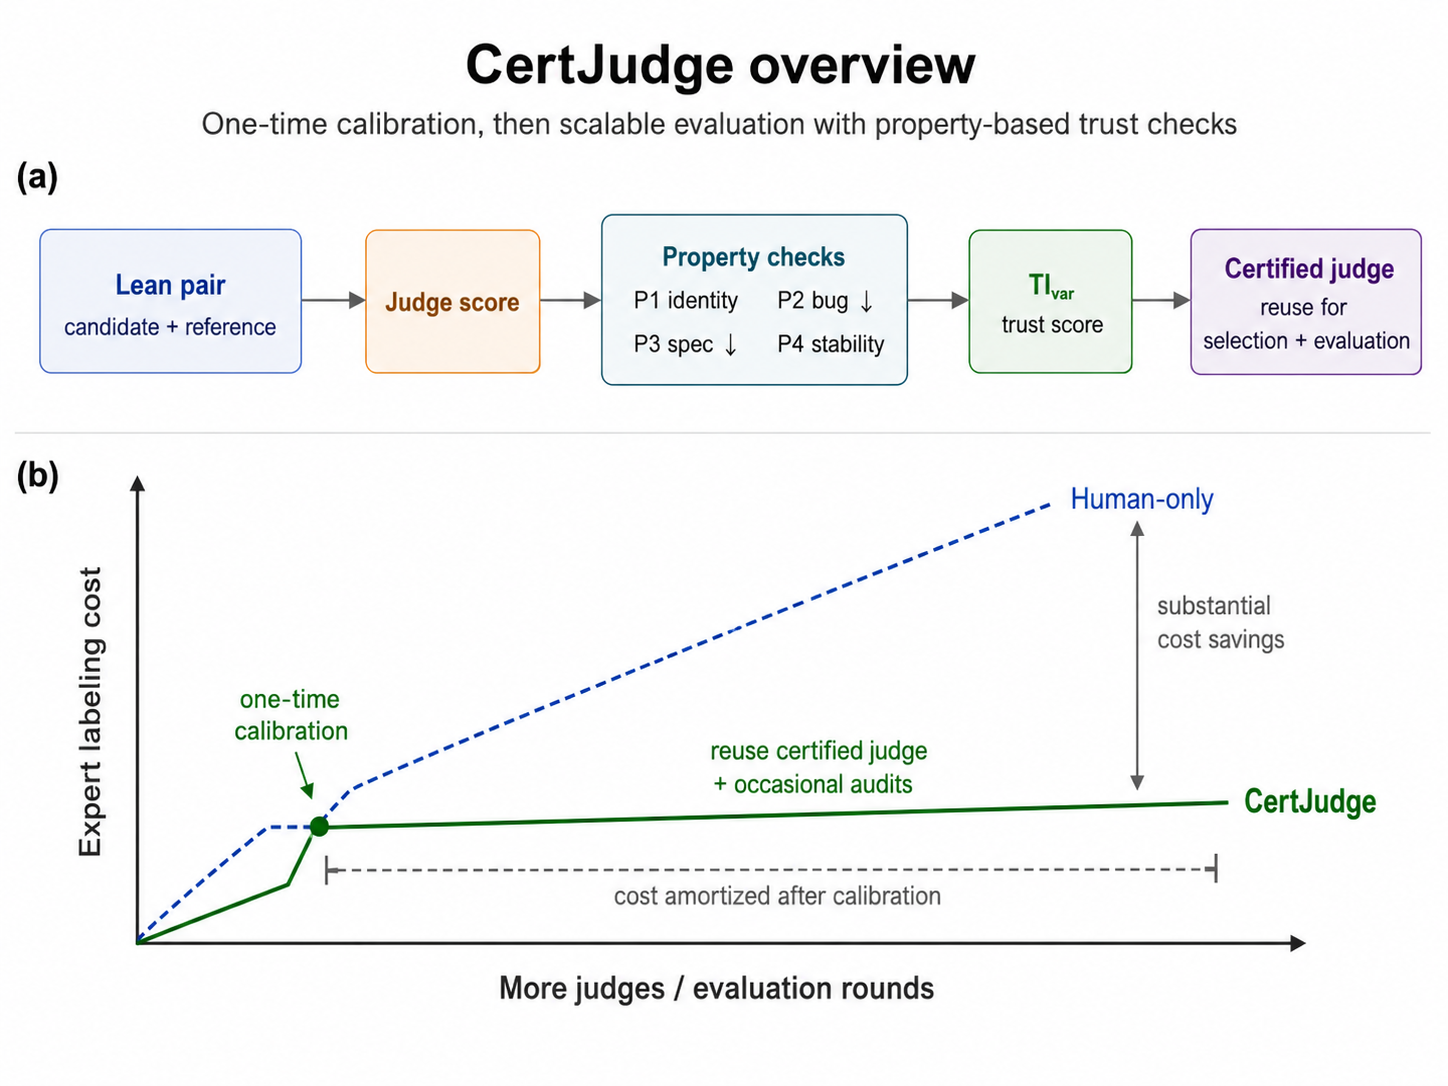
\includegraphics[width=\linewidth]{figures/pull_fig.png}
  \caption{\textbf{Scalable trust calibration for LLM judges.} A small human-labeled calibration set is paired with falsifiable property checks (P1--P4) to compute \(\mathrm{TI}_{\mathrm{var}}\), enabling judge selection and downstream evaluation with reduced relabeling overhead.}
  \label{fig:certjudge_overview}
\end{figure}

Agentic AI systems increasingly generate both code and the trust artifacts meant to evaluate that code: tests, specifications, and formal theorems.
In Lean~4, these artifacts are code-adjacent formal objects: runnable programs paired with theorem or specification statements and, sometimes, proofs that those statements hold.
In classical autoformalization, the target theorem is supplied, so evaluation can often reduce to proof success.
In agentic verification, the system must decide \emph{what should be true} before it can prove anything.
The Lean kernel can check a proof, but it cannot tell us whether the proposed theorem is complete, semantically aligned with the intended program, or merely a weak statement that happens to typecheck.
As agents produce more candidate artifacts than humans can inspect, theorem-quality evaluation becomes a code-evaluation and scalable-oversight problem \citep{bowman2022scalable,zhou2025graders,khattab2024dspy,cheng2024trace}.

The standard reliability check is per-judge human validation: collect labels, measure agreement between each judge and human ratings, and keep the judge if the correlation is high enough.
That check is necessary, but it scales linearly with the number of judges, prompts, model updates, thresholds, and domains under consideration.
Every new model family or prompt revision asks for another round of annotation, so direct human validation becomes untenable at agent-generation rates.
Humans remain the anchor; the problem is that re-using humans from scratch for every judge wastes the expensive part of the process.

% \begin{figure*}[t]
%   \centering
%   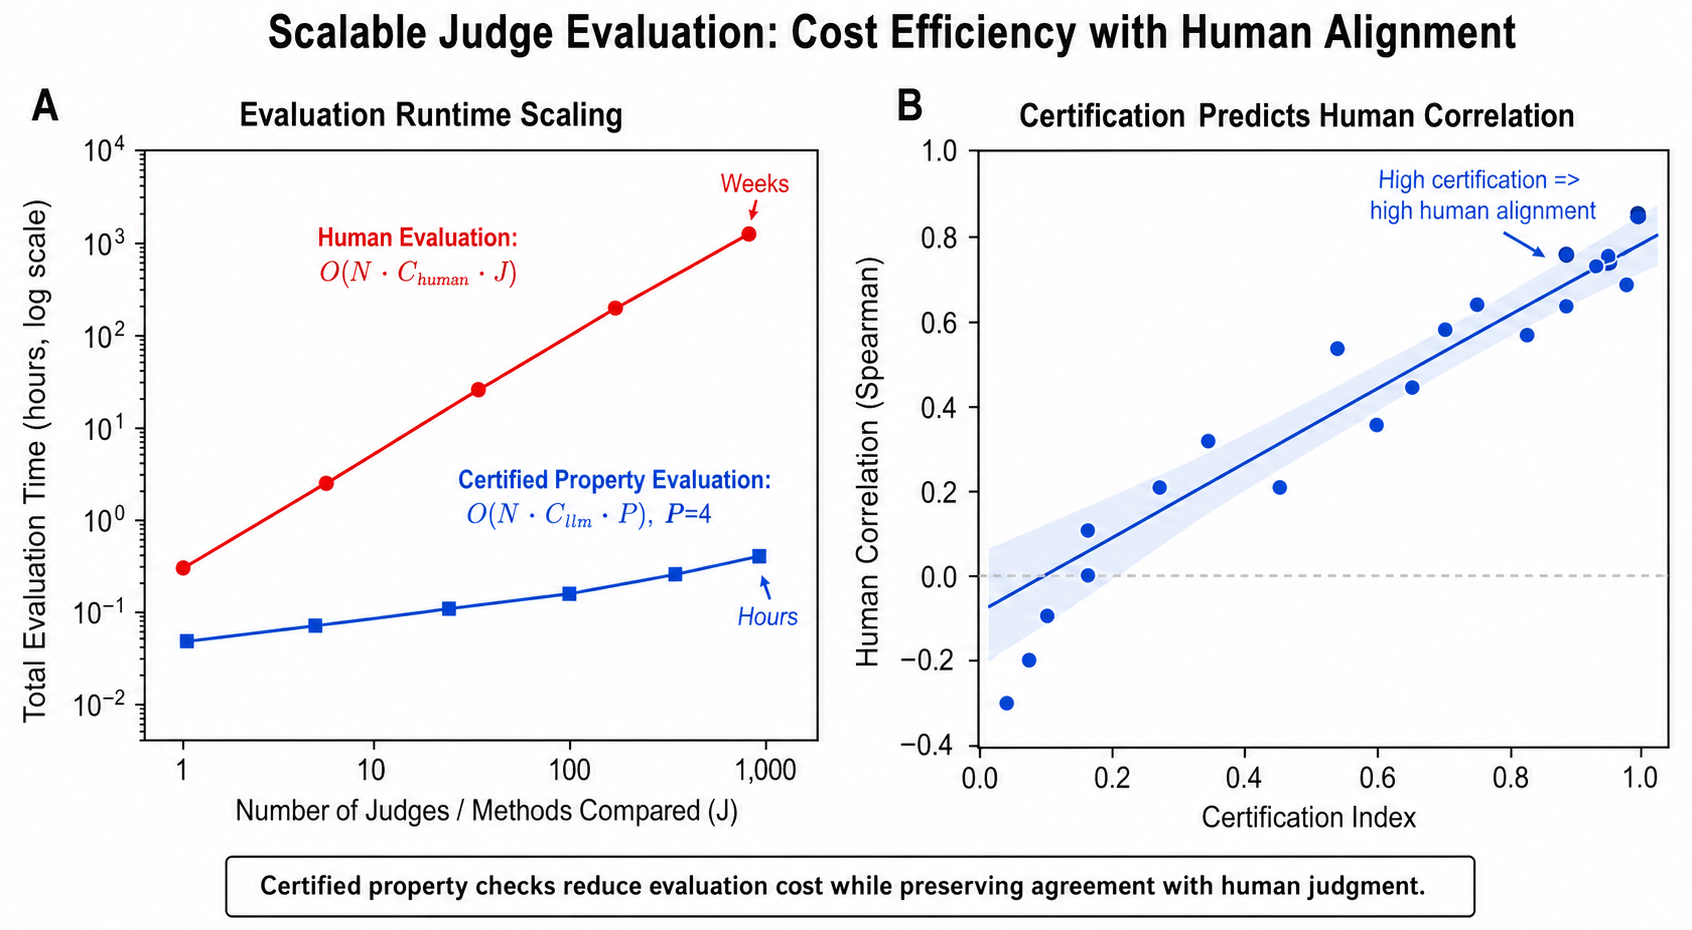
\includegraphics[width=\linewidth]{figures/pull_scalable_judge_cost_alignment.png}
%   \caption{\textbf{Scalable judge evaluation via property certification.}
%     Left: direct human validation cost scales with the number of judged methods and can become expensive at agentic throughput.
%     Right: higher certification strength is associated with higher human alignment, supporting property certification as an amortized validation protocol.}
%   \label{fig:pull_cost_alignment}
% \end{figure*}

We focus on a core \emph{AI for math} bottleneck: code agents can generate candidate formal artifacts far faster than humans can inspect them. In this setting, LLM judges are useful only if their reliability can be measured scalably rather than assumed.

Validating LLM judges against humans is the standard reliability check but does not scale: every new judge, prompt, or model needs fresh annotations.
Property certification \textbf{amortizes} this cost---gold references collected once, used to calibrate a four-property trust metric, then deployed without re-annotating every new judge configuration.
In our setting, humans rate a compact validation set once (\(n {=} 75\) aligned pairs in this proof-of-concept run), and the calibrated property suite extends that trust signal to new judges through automated property checks; the research question is whether the \emph{method} (property certification + a variance-aware index) tracks human agreement, not whether this single weighting is the final word for all domains.
The four properties are concrete: a judge should give maximal scores to identical artifacts, lower scores as semantic bugs accumulate, lower scores as theorem/test specifications are removed, and stable scores under prompt rewordings and semantics-preserving rewrites.
On a panel of eight judge configurations, \(\mathrm{TI}_{\mathrm{var}}\) fits the pooled calibration corpus with validation-set Spearman coefficients of \(0.833\) (avg labels), \(0.905\) (pass1), and \(0.738\) (pass2); held-out generalization to new raters, benchmarks, and judge families remains future work.

Our \textbf{contributions} are:
\begin{enumerate}
  \item \textbf{An amortized trust-validation protocol:} we formalize property certification as one-time calibration on a fixed panel of Lean artifacts with perturbations. After calibration, any new judge configuration can be screened by computing four falsifiable properties, without repeating the full human-labeling budget.

  \item \textbf{Proof-of-concept calibration on \(\bm{n{=}75}\):} \(\mathrm{TI}_{\mathrm{var}}\) is one geometric aggregation of diagnostics that tracks human agreement on judges; we report correlations (avg \(=0.833\), pass1 \(=0.905\), pass2 \(=0.738\) Spearman) as evidence toward amortized oversight feasibility, \emph{not} as universally fixed aggregation weights or constants.
  \item \textbf{End-to-end use on \textsc{VeriBench}:} the same calibrated judge ranks agent-generation methods consistently with benchmark expectations (e.g., DSPy ReAct \(0.615\) vs.\ baseline prompting \(0.470\) on normalized specs), illustrating how trust signals propagate to scalable code/spec evaluation workloads.
\end{enumerate}

\section{Related Work}
\paragraph{LLM-as-a-Judge.}
LLMs are increasingly used as \emph{automated evaluators} across open-ended tasks.
In prominent LLM-as-a-judge work, reliability is commonly validated by agreement with people.
\textsc{G-Eval} reports Spearman correlation with human scores \citep{Liu2023GEval}.
MT-Bench reports GPT-4 judge agreement with human preference labels \citep{Zheng2023MTBench}.
Judge-Bench evaluates whether LLMs replicate existing human annotations across 20 NLP datasets \citep{Kocmi2024HumanVsLLM}.
These studies make human agreement the standard validation target.
Our contribution keeps that target but amortizes it: one human calibration panel selects falsifiable property checks that screen future judge configurations without new labels.
However, large-scale audits caution that reliability varies by task and setup, and stress the need for explicit validation before replacing human judgment \citep{Kocmi2024HumanVsLLM,Li2024TrustLLMJudgments}.
Common biases include position and verbosity effects and sensitivity to prompt phrasing \citep{Zheng2023MTBench,Li2024TrustLLMJudgments}.

\paragraph{Improving judge reliability.}
To mitigate biases and instability, multi-agent debate frameworks such as \emph{ChatEval} emulate panel-style review to yield more robust consensus scores \citep{Chan2024ChatEval}. Structured prompting like \emph{G-Eval} elicits rubric-driven, stepwise reasoning prior to scoring, improving agreement with human criteria on NLG tasks \citep{Liu2023GEval}. Reliability can also be quantified via repeated scorings and internal consistency measures (e.g., Cronbach’s $\alpha$) to detect prompt/run sensitivity \citep{Li2024TrustLLMJudgments}.

\paragraph{Code and formal-spec evaluation.}
For programming, single-pass metrics like pass@k can be brittle or unavailable; early LLM-judge approaches such as \emph{ICE-Score} highlighted difficulty distinguishing partial vs.\ full correctness from a one-shot review \citep{Zhuo2024ICEScore}. \emph{CodeJudge} operationalizes a two-stage “analyze-then-summarize’’ procedure with a taxonomy of code faults, significantly improving correlation with functional ground truth \citep{TongZhang2024CodeJudge}. In formal verification/autoformalization, prior work typically provides fixed target theorems, reducing evaluation to proof success. In contrast, agentic systems must propose specifications, necessitating \emph{semantic} judges. We adopt a certification protocol (akin to metamorphic testing) and verify that our LLM judge obeys \emph{identity/consistency}, \emph{monotonicity} with respect to injected bugs and specification omissions, and \emph{prompt/rewrite stability}, directly answering recent calls for validated, trustworthy LLM evaluators in safety-critical domains \citep{Kocmi2024HumanVsLLM,Li2024TrustLLMJudgments}.

\paragraph{Evaluation Consistency.}
Recent work has shown that unconstrained chain-of-thought reasoning can reduce evaluation consistency, and that simple comparative prompting often outperforms complex multi-step pipelines \citep{chen2026rethinking}. We interpret these findings as evidence that stability, rather than reasoning complexity, is the primary driver of reliable grading. Our work formalizes this intuition by introducing falsifiable structural diagnostics---identity, monotonicity under controlled edits, and reliability under prompt variation---that aggregate into a graded trust signal aligned with human judgments.

\section{Evaluating Lean Theorem/Specification Quality}\label{sec:problem-setup}
\paragraph{Task.}
Each benchmark item contains a natural-language problem statement, a gold Lean~4 artifact
$g$, and a candidate artifact $x$ produced by an AI agent. The artifact may include code,
tests or specifications, and a target theorem/specification statement. Our goal is
to assign a score $J(x,g) \in [0,1]$ reflecting how well the candidate captures the intended formal specification represented
by the gold artifact.
For non-formal-methods readers, a Lean artifact is a code file in a programming language and proof assistant where executable code, tests, definitions, and theorem statements can live together.

\paragraph{Why this is nontrivial.}
Lean can check whether a concrete proof script type-checks, but type-checking alone does
not determine whether $x$ formalizes the same intended property as $g$. A candidate may
compile while being under-specified, over-constrained, vacuously true, or semantically
shifted. In \textsc{VeriBench}, this often appears as a coverage gap: candidate artifacts
may capture only part of the behavior specified by the gold reference
\citep{anonymous2026veribench}. Thus, exact automatic scoring of theorem/specification quality is unavailable in
general.

\paragraph{Judge model.}
We therefore use an LLM judge parameterized by
\[
  \theta = (\text{model}, \text{prompt}, n_{\mathrm{repeats}}, \text{aggregation}),
\]
which maps a pair $(x,g)$ to a score $J_\theta(x,g)\in[0,1]$. The central question is not
only how to build such a judge, but when it is trustworthy enough to rank systems. Rather
than collecting new human labels for every $\theta$, Section~\ref{sec:property-protocol} tests whether $J_\theta$
satisfies falsifiable behavioral constraints under controlled perturbations.

\section{Property Certification Protocol}\label{sec:property-protocol}
\subsection{Calibration Protocol}
We use property certification as a one-time calibration protocol. Humans first label a fixed reference panel; here, \(n=75\) aligned candidate--gold pairs are rated by one annotator under two rubric strictness levels. For any new judge configuration, we then compute property scores on scripted perturbations of Lean artifacts and aggregate them into a trust index, without collecting new human labels.

The judge compares a candidate Lean~4 artifact against its gold reference and returns a discrete score \(s\in\{0,1,\dots,10\}\), later normalized to \([0,1]\). The trust index is built from four property scores:
\(\text{ident}\) (P1 identity/consistency),
\(\text{mono}\) (P2 bug monotonicity),
\(\text{weak}\) (P3 specification-ablation monotonicity), and
\(\text{stab}\) (P4 repeat/prompt stability).
These are graded calibration targets, not binary gates.
As simple first-pass baselines, we also consider arithmetic variants \(v1\) and \(v2\) that aggregate these property scores without explicit variance penalties; Appendix~\ref{app:index-definitions} gives the exact formulas. These are useful comparators, but later results show that geometric and variance-aware formulations are more informative.

\textbf{Primary metric.}
\[
  \begin{aligned}
    \mathrm{TI}_{\mathrm{var}}
    ={} & \exp\!\Big(
    \tfrac{1}{3}\log C_f
    + \tfrac{1}{3}\log(1-\widetilde{\mathrm{VarCorr}}) \\
        & \qquad\quad
    + \tfrac{1}{3}\log(1-\widetilde{\mathrm{VarScore}})
    \Big),
  \end{aligned}
\]
where \(C_f\) is the geometric aggregate of the four property scores and \(\widetilde{\mathrm{VarCorr}},\widetilde{\mathrm{VarScore}}\) are normalized variance penalties; Appendix~\ref{app:index-definitions} gives the exact definitions. Our calibration claim is simple: judges with higher trust-index scores should also have higher human agreement on the validation panel. The equal-weighted form above is a simple variance-aware instantiation; other task-specific calibrations are possible, but we treat \(\mathrm{TI}_{\mathrm{var}}\) as a validation-set trust signal rather than a universal constant.

To be trustworthy, the judge should satisfy the following falsifiable calibration targets.

\paragraph{P1 — Identity \& Consistency.}
The judge should assign the maximum score to an artifact compared with itself: \(s(X,X)=1\).

\paragraph{P2 — Monotonicity to Bugs.}
Scores should decrease as semantic bugs are cumulatively introduced.

\paragraph{P3 — Monotonicity to Missing Specs.}
Scores should decrease as specification elements (theorems/tests) are removed.

\paragraph{P4 — Prompt Stability \& Semantic Invariance.}
Scores should remain stable across repeated calls and under semantics-preserving rewrites.
In particular, \textsc{Alpha}-renaming changes only bound variable names---for example, renaming local theorem variables or lambda binders without changing the proof or program structure. In ordinary programming terms, this is the kind of edit where a loop variable or local placeholder gets renamed but the program still means exactly the same thing. These edits should preserve Lean semantics exactly, so a robust judge should score the original and renamed artifact almost identically.

We evaluate these targets with rank-based monotonicity statistics (Kendall's $\tau$, Spearman's $\rho$) and pairwise ordering accuracy, following prior judge-evaluation work \citep{TongZhang2024CodeJudge,Zhuo2024ICEScore}.

\begin{table}[t]
  \centering
  \small
  \begin{tabular}{@{}r@{\kern 7pt}>{\raggedright\arraybackslash} p{0.89\linewidth}@{}}
    \toprule
    \textbf{Step} & \textbf{Action}                                                                                                                                                                                                                                                                                      \\
    \midrule
    1             &
    Collect a diverse set of human ratings on candidate-vs.-gold Lean artifacts (\(n{=}75\) in our calibration).                                                                                                                                                                                                         \\
    2             &
    For each candidate judge, evaluate identity, bug-monotonicity, spec-monotonicity, and stability on Lean artifacts subjected to agent-scripted perturbations; grading these properties uses only automated ladders and judge runs on perturbed artifacts—\emph{not} pairwise human-vs.-gold labels on those variants. \\
    3             &
    Combine how well properties are satisfied with explicit instability penalties into the variance-aware trust index \(\mathrm{TI}_{\mathrm{var}}\).                                                                                                                                                                    \\
    4             &
    Prefer judge tuples with higher \(\mathrm{TI}_{\mathrm{var}}\) for larger-scale code/spec judging and deployment.                                                                                                                                                                                                    \\
    \bottomrule
  \end{tabular}
  \caption{\textbf{Property-certification workflow.}
    A one-time human panel calibrates the relationship between falsifiable judge properties
    and human agreement; subsequent judge configurations can be screened automatically.}
  \label{tab:protocol_workflow}
\end{table}

\begin{figure*}[t]
  \centering
  \captionsetup[subfigure]{font=small,labelfont=bf,justification=centering}
  \begin{subfigure}[t]{0.315\textwidth}
    \centering
    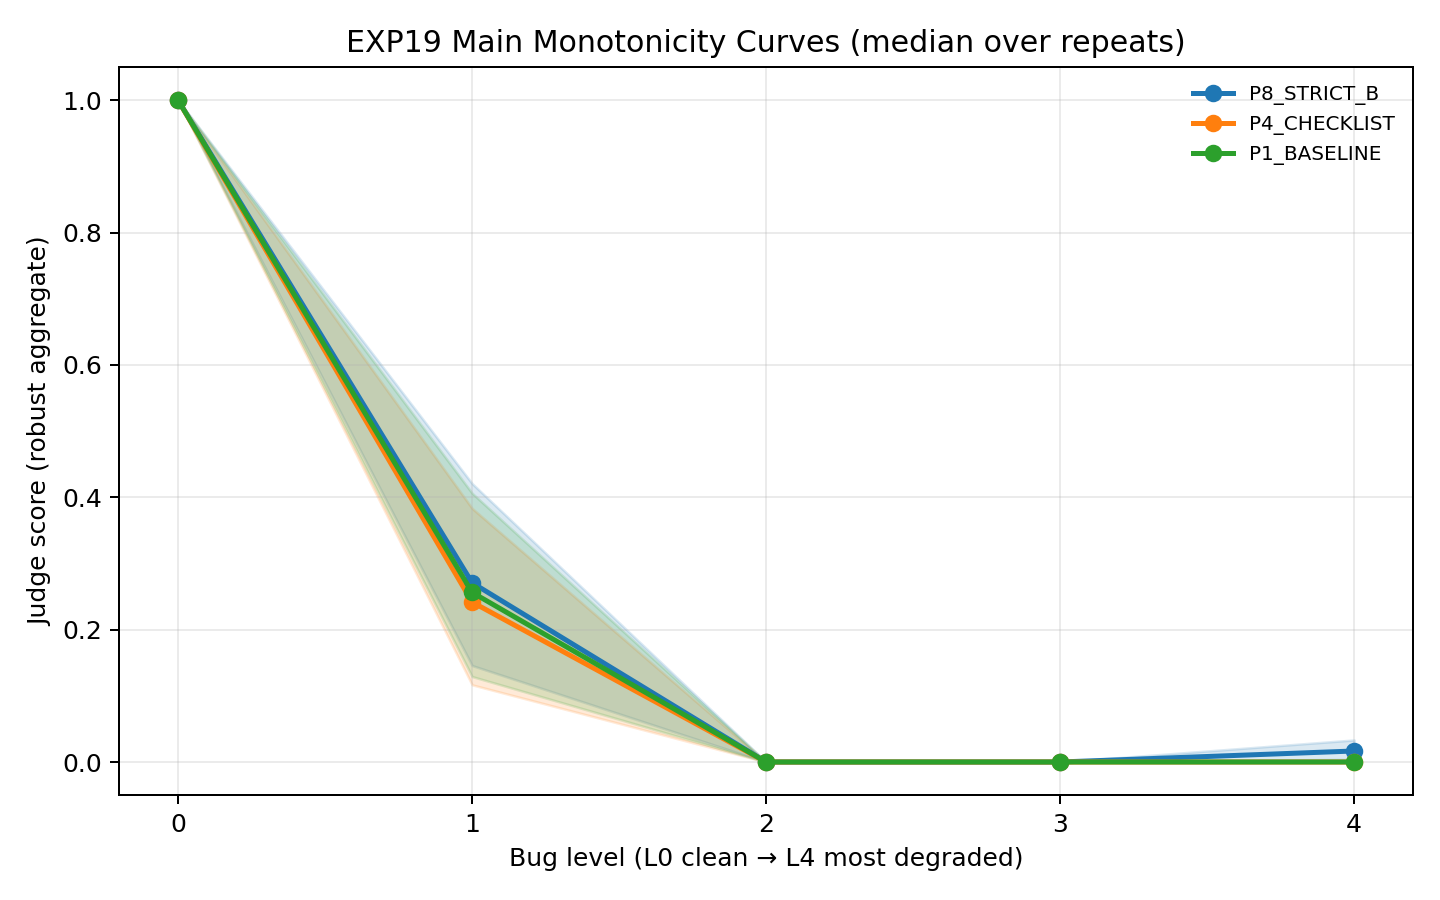
\includegraphics[width=\linewidth]{figures/fig_main_monotonicity_lowvar_exp19.png}
    \caption{Average score under increasing degradation}
    \label{fig:judge_lowvar_main}
  \end{subfigure}\hfill
  \begin{subfigure}[t]{0.315\textwidth}
    \centering
    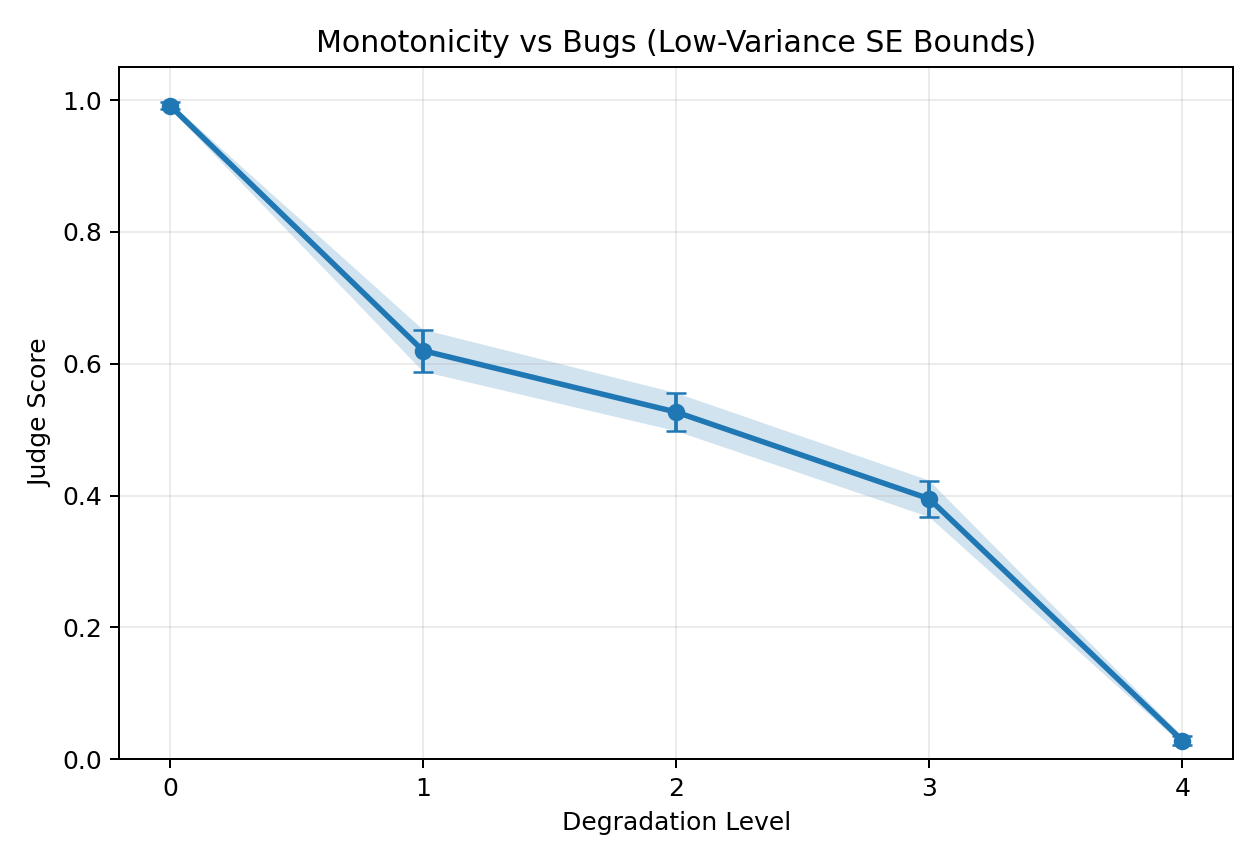
\includegraphics[width=\linewidth]{figures/codex_api_gpt53_r3_20260418_230027/monotonicity_bugs_lowvar_se_bounds.png}
    \caption{P2: Monotonicity vs.\ Bugs (Mean \(\pm\) SE)}
    \label{fig:judge_mono_bugs}
  \end{subfigure}\hfill
  \begin{subfigure}[t]{0.315\textwidth}
    \centering
    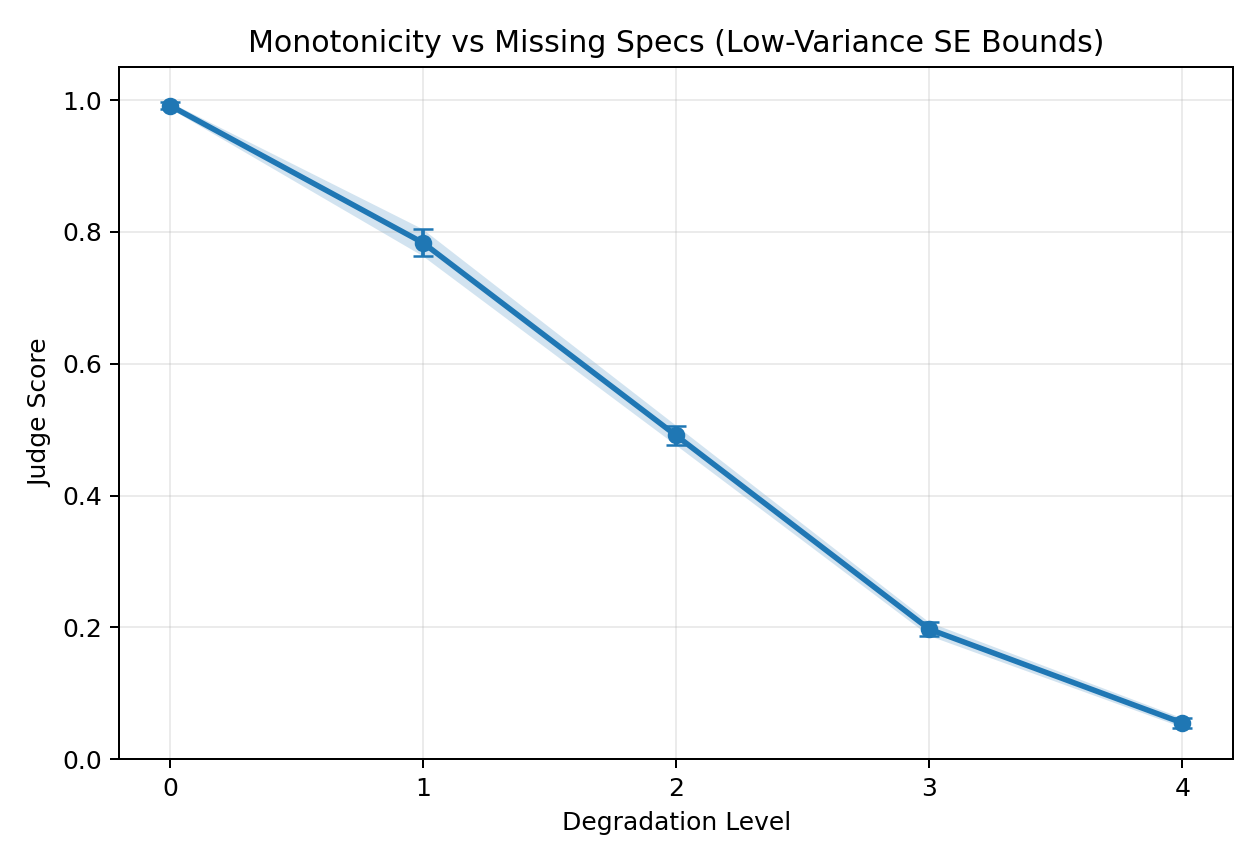
\includegraphics[width=\linewidth]{figures/codex_api_gpt53_r3_20260418_230027/monotonicity_missing_specs_lowvar_se_bounds.png}
    \caption{P3: Monotonicity vs.\ Missing Specs (Mean \(\pm\) SE)}
    \label{fig:judge_mono_specs}
  \end{subfigure}
  \vspace{-2mm}
  \caption{\textbf{LLM Judge Trustworthiness Sanity Checks.}
    VeriBench-wide GPT-5.3-Codex API run (\(n_\text{files}=184\), \(n_\text{repeats}=3\)).
    \textbf{(a)} Low-variance rendering emphasizes smooth non-increasing score behavior under controlled degradations.
    \textbf{(b)} P2 bug-ladder trend remains directionally correct with local reversals (Pearson \(r=-0.687\), Spearman \(\rho=-0.808\), weak monotonicity \(52.2\%\)).
    \textbf{(c)} P3 missing-spec trend is stronger and more stable (Pearson \(r=-0.892\), Spearman \(\rho=-0.899\), weak monotonicity \(89.1\%\)).
    Strict P1 identity \(s(X,X)\) and P4 rewrite invariance are reported separately in Table~\ref{tab:codex_invariance_variants}.}
  \label{fig:judge_sanity_checks}
  \vspace{-3mm}
\end{figure*}

\section{Experiments}
\subsection{Data and human-validation protocol}\label{sec:data-human-protocol}\label{sec:veribench-overview}
All experiments use \textsc{VeriBench}~\citep{anonymous2026veribench}.

\paragraph{Overview of \textsc{VeriBench}.}
Concretely, \textsc{VeriBench} consists of 857 theorems divided into five subsets:
\begin{enumerate}
  \item \textbf{HumanEval} -- 387 theorems derived from 56 standard programming puzzles from \citet{chen2021evaluating};
  \item \textbf{EasySet} -- 278 theorems extracted from 41 introductory logic and programming tasks;
  \item \textbf{CSSet} -- 68 theorems drawn from 10 classical data-structure and algorithm problems;
  \item \textbf{SecuritySet} -- 112 theorems taken from 28 examples of buffer overflows, privilege escalation, and race-condition labs based on real code;
  \item \textbf{RealCodeSet} -- 12 theorems extracted from 5 Python standard library programs, used to test model performance on production-grade code.
\end{enumerate}
We map these to shorthand subset names \textbf{Easy}, \textbf{CS}, \textbf{HumanEval}, \textbf{Security}, and \textbf{RealCode}. This design spans simple correctness routines through security-relevant invariants and excerpts of production library code.

For judge-validation, we use an aligned panel of \(n=75\) candidate--gold pairs from \(24\) problems with \(3\) agent generations per problem. Each pair receives two human passes on a \(0\)--\(5\) rubric, and we report pass1, pass2, and averaged labels.

The same aligned panel is reused across judges, so differences in trend reflect judge behavior rather than row selection. Human-pass dispersion is non-trivial (Appendix Figure~\ref{fig:app-human-pass-hist}), which is why we report all three label views rather than a single pass.

\subsection{Property sanity checks on GPT-5.3-Codex}
\textbf{Establishing trust in the judge.} Figure~\ref{fig:judge_sanity_checks} shows that the Codex judge satisfies the intended qualitative behavior: scores decrease as semantic bugs accumulate and as specifications are removed, while identity and rewrite robustness are handled separately through P1/P4 diagnostics. The strongest signal is specification-ablation monotonicity (\(\rho=-0.899\), \(r=-0.892\)); bug monotonicity is also directionally correct but noisier (\(\rho=-0.808\), \(r=-0.687\)), indicating occasional local reversals. Appendix Figures~\ref{fig:fig3_style_opus_codex} and~\ref{fig:lowvar_mono_codex_opus} show that the same monotone degradation pattern is also visible for Claude Opus under matched plotting protocols.

\begin{table}[t]
  \centering
  \scriptsize
  \begin{tabular}{lcc}
    \toprule
    \textbf{Identity Variant} & \textbf{Mean Score} & \textbf{Mean Within-Item Std} \\
    \midrule
    RENAME                    & 0.936               & 0.005                         \\
    REORDER                   & 0.849               & 0.029                         \\
    STYLE                     & 0.982               & 0.001                         \\
    ALPHA                     & 0.399               & 0.096                         \\
    \bottomrule
  \end{tabular}
  \caption{\textbf{P4 semantic-invariance breakdown for the Codex API run.}
    Variant-wise score behavior under semantics-preserving rewrites. The weakest mode is aggressive \textsc{Alpha}-renaming.}
  \label{tab:codex_invariance_variants}
\end{table}

These sanity checks support using the judge as a semantically meaningful proxy for theorem/specification quality, while also making the main failure mode explicit: aggressive \textsc{Alpha}-renaming remains substantially less stable than milder rewrites. Rankings under repeat-resampled scores are stable enough to aggregate into a trust index, but \textsc{Alpha}-renaming stays the dominant identity gap (Figure~\ref{fig:app-exp19-main-and-alpha}).

\subsection{\texorpdfstring{\(\mathrm{TI}_{\mathrm{var}}\)}{TI-var} predicts judge-level human alignment}
\label{sec:tivar_cross_model_results}
\label{sec:validation-human-alignment}

A central question for our protocol is whether the primary trust metric \(\mathrm{TI}_{\mathrm{var}}\) yields a calibrated signal that aligns with how humans judge candidate Lean artifacts under the same rubric. We do \emph{not} claim that \(\mathrm{TI}_{\mathrm{var}}\) certifies universally correct evaluator behavior---no finite scripted suite can enumerate all plausible failure modes (Section~\ref{sec:limitations-finite}).

Across Codex, Claude Opus, and Qwen3-Coder, judges with higher \(\mathrm{TI}_{\mathrm{var}}\) also have higher correlation with human ratings. Figure~\ref{fig:tivar_cross_model_avg} plots judge-level \(\mathrm{TI}_{\mathrm{var}}\) against human Spearman agreement (averaged validation labels) separately for those three judge families while holding fixed the \(75\) overlapping human-aligned rows that define the calibration panel within each regression. \(\mathrm{TI}_{\mathrm{var}}\) does not only reward average property satisfaction---it also penalizes instability across repeats, prompts, and perturbations---so the signal targets configurations that behave more coherently on the perturbation suite used for calibration.

\begin{figure*}[t]
  \centering
  {\footnotesize\textbf{\(\mathrm{TI}_{\mathrm{var}}\) vs Human Agreement (Avg Labels): Codex / Claude Opus / Qwen3-Coder}\\[2.5mm]}
  \definecolor{jP8}{HTML}{1F77B4}%
  \definecolor{jP4}{HTML}{2CA02C}%
  \definecolor{jP1}{HTML}{FF7F0E}%
  \definecolor{jBAD}{HTML}{D62728}%
  \definecolor{jIVP8}{HTML}{9467BD}%
  \definecolor{jIVP4}{HTML}{8C564B}%
  \definecolor{jedit}{HTML}{7F7F7F}%
  \definecolor{jrand}{HTML}{BCBD22}%
  \noindent
  \centering
  \begin{subfigure}[t]{0.323\textwidth}
    \centering
    \begin{tikzpicture}
      \begin{axis}[
        width=\linewidth,
        height=5.05cm,
        clip=false,
        xmin=0, xmax=1.0,
        ymin=-0.1, ymax=0.62,
        xlabel={\(\mathrm{TI}_{\mathrm{var}}\)},
        ylabel={Human Spearman (avg)},
        title={\parbox{\linewidth}{\centering Codex $\rho=0.833$}},
        title style={font=\small},
        grid=major,
        grid style={draw=gray!20},
        tick label style={font=\scriptsize},
        label style={font=\scriptsize},
        legend pos=north west,
        legend columns=2,
        legend cell align=left,
        legend style={
            font=\fontsize{7}{8}\selectfont,
            draw=gray!50,
            fill=white,
            fill opacity=0.94,
            text opacity=1,
            inner sep=2pt,
            column sep=3.5pt,
            row sep=1.5pt,
          },
        ]
        \addplot+[only marks, mark=*, mark size=1.65pt, color=jrand,
          error bars/.cd, y dir=both, y explicit]
        coordinates {(0.0083,-0.0008) +- (0,0.0684)};
        \addlegendentry{rand}
        \addplot+[only marks, mark=*, mark size=1.65pt, color=jedit,
          error bars/.cd, y dir=both, y explicit]
        coordinates {(0.0595,0.1987) +- (0,0.0769)};
        \addlegendentry{edit}
        \addplot+[only marks, mark=*, mark size=1.65pt, color=jIVP4,
          error bars/.cd, y dir=both, y explicit]
        coordinates {(0.1141,0.0916) +- (0,0.0697)};
        \addlegendentry{4o-P4}
        \addplot+[only marks, mark=*, mark size=1.65pt, color=jIVP8,
          error bars/.cd, y dir=both, y explicit]
        coordinates {(0.4709,-0.0142) +- (0,0.0702)};
        \addlegendentry{4o-P8}
        \addplot+[only marks, mark=*, mark size=1.65pt, color=jBAD,
          error bars/.cd, y dir=both, y explicit]
        coordinates {(0.6964,0.4348) +- (0,0.0635)};
        \addlegendentry{BAD}
        \addplot+[only marks, mark=*, mark size=1.65pt, color=jP1,
          error bars/.cd, y dir=both, y explicit]
        coordinates {(0.9208,0.4664) +- (0,0.0588)};
        \addlegendentry{P1}
        \addplot+[only marks, mark=*, mark size=1.65pt, color=jP4,
          error bars/.cd, y dir=both, y explicit]
        coordinates {(0.9199,0.4193) +- (0,0.0614)};
        \addlegendentry{P4}
        \addplot+[only marks, mark=*, mark size=1.65pt, color=jP8,
          error bars/.cd, y dir=both, y explicit]
        coordinates {(0.8919,0.3652) +- (0,0.0683)};
        \addlegendentry{P8}
        \addplot+[domain=0.0083:0.9208, samples=2, dashed, color=red!65!black, thick, forget plot] {0.5080*x - 0.0128};
      \end{axis}
    \end{tikzpicture}
  \end{subfigure}\hfill
  \begin{subfigure}[t]{0.323\textwidth}
    \centering
    \begin{tikzpicture}
      \begin{axis}[
        width=\linewidth,
        height=5.05cm,
        clip=false,
        xmin=0, xmax=1.0,
        ymin=-0.1, ymax=0.62,
        xlabel={\(\mathrm{TI}_{\mathrm{var}}\)},
        title={\parbox{\linewidth}{\centering Claude Opus $\rho=0.643$}},
        title style={font=\small},
        grid=major,
        grid style={draw=gray!20},
        tick label style={font=\scriptsize},
        label style={font=\scriptsize},
        ]
        \addplot+[only marks, mark=*, mark size=1.65pt, color=jrand,
          error bars/.cd, y dir=both, y explicit]
        coordinates {(0.0083,-0.0008) +- (0,0.0672)};
        \addplot+[only marks, mark=*, mark size=1.65pt, color=jedit,
          error bars/.cd, y dir=both, y explicit]
        coordinates {(0.0595,0.1987) +- (0,0.0772)};
        \addplot+[only marks, mark=*, mark size=1.65pt, color=jIVP4,
          error bars/.cd, y dir=both, y explicit]
        coordinates {(0.1134,0.1910) +- (0,0.0668)};
        \addplot+[only marks, mark=*, mark size=1.65pt, color=jIVP8,
          error bars/.cd, y dir=both, y explicit]
        coordinates {(0.5585,0.0888) +- (0,0.0738)};
        \addplot+[only marks, mark=*, mark size=1.65pt, color=jBAD,
          error bars/.cd, y dir=both, y explicit]
        coordinates {(0.7458,0.3243) +- (0,0.0604)};
        \addplot+[only marks, mark=*, mark size=1.65pt, color=jP1,
          error bars/.cd, y dir=both, y explicit]
        coordinates {(0.9284,0.3153) +- (0,0.0702)};
        \addplot+[only marks, mark=*, mark size=1.65pt, color=jP4,
          error bars/.cd, y dir=both, y explicit]
        coordinates {(0.9270,0.4514) +- (0,0.0614)};
        \addplot+[only marks, mark=*, mark size=1.65pt, color=jP8,
          error bars/.cd, y dir=both, y explicit]
        coordinates {(0.9474,0.1453) +- (0,0.0730)};
        \addplot+[domain=0.0083:0.9474, samples=2, dashed, color=red!65!black, thick, forget plot] {0.2776*x + 0.0571};
      \end{axis}
    \end{tikzpicture}
  \end{subfigure}\hfill
  \begin{subfigure}[t]{0.323\textwidth}
    \centering
    \begin{tikzpicture}
      \begin{axis}[
        width=\linewidth,
        height=5.05cm,
        clip=false,
        xmin=0, xmax=1.0,
        ymin=-0.1, ymax=0.62,
        xlabel={\(\mathrm{TI}_{\mathrm{var}}\)},
        title={\parbox{\linewidth}{\centering Qwen3-Coder $\rho=0.905$}},
        title style={font=\small},
        grid=major,
        grid style={draw=gray!20},
        tick label style={font=\scriptsize},
        label style={font=\scriptsize},
        ]
        \addplot+[only marks, mark=*, mark size=1.65pt, color=jrand,
          error bars/.cd, y dir=both, y explicit]
        coordinates {(0.0083,-0.0008) +- (0,0.0672)};
        \addplot+[only marks, mark=*, mark size=1.65pt, color=jedit,
          error bars/.cd, y dir=both, y explicit]
        coordinates {(0.0595,0.1987) +- (0,0.0772)};
        \addplot+[only marks, mark=*, mark size=1.65pt, color=jIVP4,
          error bars/.cd, y dir=both, y explicit]
        coordinates {(0.1267,0.0759) +- (0,0.0722)};
        \addplot+[only marks, mark=*, mark size=1.65pt, color=jIVP8,
          error bars/.cd, y dir=both, y explicit]
        coordinates {(0.7059,0.0789) +- (0,0.0703)};
        \addplot+[only marks, mark=*, mark size=1.65pt, color=jP1,
          error bars/.cd, y dir=both, y explicit]
        coordinates {(0.8860,0.1742) +- (0,0.0756)};
        \addplot+[only marks, mark=*, mark size=1.65pt, color=jP4,
          error bars/.cd, y dir=both, y explicit]
        coordinates {(0.8869,0.3603) +- (0,0.0585)};
        \addplot+[only marks, mark=*, mark size=1.65pt, color=jP8,
          error bars/.cd, y dir=both, y explicit]
        coordinates {(0.9396,0.1207) +- (0,0.0724)};
        \addplot+[only marks, mark=*, mark size=1.65pt, color=jBAD,
          error bars/.cd, y dir=both, y explicit]
        coordinates {(0.9420,0.3705) +- (0,0.0649)};
        \addplot+[domain=0.0083:0.9420, samples=2, dashed, color=red!65!black, thick, forget plot] {0.2337*x + 0.0687};
      \end{axis}
    \end{tikzpicture}
  \end{subfigure}
  \caption{\textbf{$\mathrm{TI}_{\mathrm{var}}$ vs.\ judge-level human alignment.}
  Each point is one judge configuration; the \(x\)-axis is \(\mathrm{TI}_{\mathrm{var}}\), and the \(y\)-axis is Spearman agreement with averaged human labels on the aligned validation panel.
  Vertical bars show approximate bootstrap SE; dashed lines are OLS guides.
  Across model families, higher certification strength tracks higher human alignment.}
  \label{fig:tivar_cross_model_avg}
  \vspace{-2mm}
\end{figure*}

\begin{table}[t]
  \centering
  \small
  \begin{tabular}{lccc}
    \toprule
    \textbf{Model Family} & \textbf{pass1} & \textbf{pass2} & \textbf{avg} \\
    \midrule
    Codex                 & 0.905          & 0.738          & 0.833        \\
    Claude Opus           & 0.810          & 0.595          & 0.643        \\
    Qwen3-Coder           & 0.476          & 0.905          & 0.905        \\
    \bottomrule
  \end{tabular}
  \caption{\textbf{Judge-level \(\mathrm{TI}_{\mathrm{var}}\rightarrow\) human alignment.}
  Spearman correlation between judge-level \(\mathrm{TI}_{\mathrm{var}}\) and judge-level human Spearman agreement on the aligned panel. Pass-specific values differ across rubric severity; the qualitative pattern is stable across families.}
  \label{tab:tivar_cross_model_results}
\end{table}

Table~\ref{tab:tivar_cross_model_results} reports the same relationship for pass1, pass2, and averaged labels. Codex is strongest on pass1 and avg, Qwen strongest on pass2 and avg, and Claude Opus stays positive on all three. The point is not that one family dominates every split; it is that the same certification signal remains informative across distinct judge families. Most coefficients are large in magnitude---six of nine family/pass combinations exceed \(0.7\).

However, because the judge-level trend is estimated over a small panel, we treat the effect size as calibration evidence and report cross-pass and cross-family robustness rather than claiming deployment-ready generalization.

For the Codex calibration panel (\(n=8\) judges), Pearson shows the same qualitative pattern (avg \(r=0.774\), pass1 \(r=0.661\), pass2 \(r=0.837\)), while Kendall \(\tau\) is noisier at this scale (avg \(\tau=0.571\), pass1 \(\tau=0.571\), pass2 \(\tau=0.643\)).

Thus \(\mathrm{TI}_{\mathrm{var}}\) behaves as a calibrated reliability signal: falsifiable properties correlate with the quantity we care about---agreement with human assessments of Lean theorem and specification quality---so new judge configurations can be compared by automated property checks after the calibration relationship is measured once.

\paragraph{Human-pass dispersion and cross-pass robustness.}
Annotators scored each aligned pair twice under different rubric strictness. Agreement between passes is moderate (Spearman \(=0.249\), Pearson \(=0.375\), quadratic-weighted kappa (QWK) \(=0.372\), MAE \(=0.778\) on the \(0\)--\(5\) scale), so judge--human numbers are calibration evidence rather than ceiling performance. Table~\ref{tab:app-human-human-ceiling} gathers full diagnostics.

\begin{table}[t]
  \centering
  \small
  \begin{tabular}{lcc}
    \toprule
    \textbf{Protocol}           & \makecell{\textbf{Fit}         \\ \textbf{Spearman}}  & \makecell{\textbf{Test} \\ \textbf{Spearman}} \\
    \midrule
    pass1 \(\rightarrow\) pass2 & 0.881                  & 0.810 \\
    pass2 \(\rightarrow\) pass1 & 0.857                  & 0.786 \\
    \bottomrule
  \end{tabular}
  \caption{\textbf{Cross-pass robustness.}
  \emph{Fit Spearman}: judge-level Spearman\((\mathrm{TI}_{\mathrm{var}},\) human alignment\()\) when weights are tuned on one pass.
  \emph{Test Spearman}: the same statistic on the other pass.}
  \label{tab:cross_pass_generalization}
\end{table}

Table~\ref{tab:cross_pass_generalization} shows that test Spearman stays above \(0.7\) in both directions when \(\mathrm{TI}_{\mathrm{var}}\) is fit using one human pass alone.

\subsection{Why \texorpdfstring{\(\mathrm{TI}_{\mathrm{var}}\)}{TI-var} is the primary trust metric}
Figure~\ref{fig:tivar_cross_model_avg} with Table~\ref{tab:tivar_cross_model_results} states the headline cross-family trend. Table~\ref{tab:cross_model_index_compare_avg} then asks a narrower question: which trust-index formulation best captures that trend on averaged labels? Relative to arithmetic baselines, \(\mathrm{TI}_{\mathrm{var}}\) uniformly improves over \(v2\) for every family: Codex \(0.476\!\rightarrow\!0.833\), Claude Opus \(0.143\!\rightarrow\!0.643\), Qwen3-Coder \(0.500\!\rightarrow\!0.905\). The geometric index (GM) is competitive for Codex and Opus (\(0.857\) and \(0.714\) respectively), while \(\mathrm{TI}_{\mathrm{var}}\) stays most consistently strong across families and is the strongest formulation for Qwen. These comparisons suggest that a variance-aware trust metric can track human alignment more reliably than simpler arithmetic aggregation, while geometric aggregation also improves over the arithmetic baseline. We therefore adopt \(\mathrm{TI}_{\mathrm{var}}\) as the paper's primary metric because it combines property quality with explicit variance penalties while yielding positive judge-level trends everywhere we test. Figure~\ref{fig:app-exp25-13judge} provides a baseline-vs-geometric visualization on an expanded judge panel.

\begin{table}[t]
  \centering
  \small
  \begin{tabular}{lcccc}
    \toprule
    \textbf{Model} & \textbf{v1} & \textbf{v2} & \textbf{GM} & $\mathrm{TI}_{\mathrm{var}}$ \\
    \midrule
    Codex          & 0.762       & 0.476       & 0.857       & 0.833                        \\
    Claude Opus    & 0.429       & 0.143       & 0.714       & 0.643                        \\
    Qwen3-Coder    & 0.524       & 0.500       & 0.786       & 0.905                        \\
    \bottomrule
  \end{tabular}
  \caption{\textbf{Avg-label judge-level trends by trust-index formulation.}
  Spearman correlation between index score and per-judge human Spearman on averaged labels.
  \(v1\) and \(v2\): arithmetic variants; GM: geometric monotonicity/stability; \(\mathrm{TI}_{\mathrm{var}}\): variance-aware index.}
  \label{tab:cross_model_index_compare_avg}
\end{table}

\paragraph{Takeaway for calibrated code evaluation.}
The main empirical claim is not that any finite property suite certifies judge correctness. Rather, the claim is that falsifiable diagnostics can predict which LLM judges agree more strongly with human assessments of formal-code artifacts. This matters for AI for math because code agents can generate far more tests, specifications, and theorems than humans can inspect, while a one-time human calibration panel plus automated property checks provides a scalable way to compare judge configurations before deploying them on larger agent evaluations.

\paragraph{Property-level interpretation.}
For averaged labels, per-property correlations identify
\textbf{P3 weak monotonicity} as strongest (Spearman \(0.747,\ p=0.043\); Pearson \(0.744,\ p=0.048\)),
with \textbf{P2 bug-rank monotonicity} next (Spearman \(0.714,\ p=0.056\); Pearson \(0.636,\ p=0.037\)).
P1 identity and P4 stability are not strong standalone predictors at this \(n_\text{judges}=8\) scale.
Across pass1/pass2/avg, P3 is consistently top-ranked, indicating that semantic monotone behavior under controlled degradations is the most stable predictor of validation-set human Spearman in this study.

\subsection{Threshold calibration: stability vs.\ coverage}
\paragraph{Decision-threshold calibration.}
After validating score-level behavior, we calibrate a binary operating point for deployment. A threshold \(t\) converts a continuous judge score into a yes/no decision, and flip rate measures how often repeated judge calls on the same item disagree after thresholding. Across \(t\in\{0.60,0.65,0.70,0.75,0.80,0.85\}\), ranking behavior is essentially unchanged (\(\rho_{\text{bug}}=-0.790\) throughout), while stricter thresholds modestly reduce flip rate at the cost of lower coverage. We therefore select \(t=0.85\), which yields the lowest observed flip rate while keeping pass rate near \(0.5\) (Table~\ref{tab:exp13_threshold_sweep}).

\begin{table}[t]
  \centering
  \small
  \begin{tabular}{lcc}
    \toprule
    \textbf{Threshold} & \textbf{Flip Rate (95\% CI)}                        & \textbf{Pass Rate (95\% CI)} \\
    \midrule
    0.60               & 0.058 \([0.048, 0.069]\)                            & 0.583 \([0.559, 0.608]\)     \\
    0.70               & 0.049 \([0.040, 0.059]\)                            & 0.559 \([0.537, 0.581]\)     \\
    0.80               & 0.051 \([0.042, 0.061]\)                            & 0.544 \([0.523, 0.566]\)     \\
    0.85               & \textbf{0.046} \([\textbf{0.037}, \textbf{0.057}]\) & 0.536 \([0.515, 0.557]\)     \\
    \bottomrule
  \end{tabular}
  \caption{\textbf{Threshold calibration summary.}
    Calibration yields a modest but consistent reduction in decision flips at stricter thresholds, with moderate coverage loss.
    Ranking behavior is unchanged across thresholds (\(\rho_{\text{bug}}=-0.790\) at all \(t\)).}
  \label{tab:exp13_threshold_sweep}
\end{table}

\subsection{Failure modes: alpha-renaming and local reversals}
The main failure mode remains the same throughout the study: alpha-renaming is substantially less stable than milder rewrites, and local monotonicity reversals can still occur even when global trends are strong. Alpha-renaming is intentionally a weak perturbation---it should leave theorem quality unchanged---so failures here are informative about superficial sensitivity rather than true semantic degradation. At the same time, it is a hard robustness target, because changing binder names can alter token patterns and local readability cues even when Lean semantics are unchanged. On an expanded 13-judge panel, the certification trend remains above \(0.75\) across label sets, suggesting that the effect is not specific to a minimal prompt panel. Detailed per-model diagnostics are reported in the appendix.

\begin{table}[H]
  \renewcommand{\arraystretch}{1.30}
  \centering
  \resizebox{\columnwidth}{!}{%
    \begin{tabular}{@{}lcccccc@{}}
      \toprule
      \textbf{Agent}      & \textbf{Easy} & \textbf{CS} & \textbf{Real} & \textbf{HE} & \textbf{Sec} & \textbf{Avg}   \\
      \midrule
      Baseline            & 0.580         & 0.690       & 0.472         & 0.410       & 0.347        & \textbf{0.470} \\
      \addlinespace[2pt]
      \hdashline[0.5pt/4pt]
      \addlinespace[2pt]
      \textsc{DSPy ReAct} & 0.659         & 0.754       & 0.580         & 0.650       & 0.454        & \textbf{0.615} \\
      \addlinespace[2pt]
      \hdashline[0.5pt/4pt]
      \addlinespace[2pt]
      \textsc{Trace+}     & 0.342         & 0.680       & 0.592         & 0.573       & 0.411        & \textbf{0.477} \\
      \addlinespace[2pt]
      \hdashline[0.5pt/4pt]
      \addlinespace[2pt]
      \textsc{Trace++}    & 0.620         & 0.756       & 0.504         & 0.645       & 0.432        & \textbf{0.588} \\
      \bottomrule
    \end{tabular}%
  }
  \caption{\textbf{Theorem quality scores on \textsc{VeriBench}.} Average normalized scores by split: Easy, CS, Real, HumanEval, and Security.
    All rows use Claude~3.7 as the agent model and as the LLM judge.
    Trace+ denotes the trace self-debug agent and Trace++ the self-debug and self-improve agent.
    The DSPy ReAct agent only performs self-debug.
    The LLM judge issues 5 scoring calls per file pair and returns an integer rubric score in $\{0,1,\dots,10\}$.
    Normalized scores are computed by dividing by the maximum score (10) and averaging across all examples.
    The Avg Norm Score shows the overall average over the entire benchmark.}
  \label{tab:theorem_quality_table_split}
\end{table}

\subsection{Downstream \textsc{VeriBench} agent ranking}
The calibrated judge is useful not only as a validation object but also as an evaluation tool. Table~\ref{tab:theorem_quality_table_split} shows that it ranks agentic theorem-generation methods in the expected direction: the weakest baseline is simple prompting (0.470 average normalized score), while feedback-driven methods score substantially higher, led by DSPy ReAct (0.615) and followed by Trace++ (0.588). We use this only as a downstream sanity check, not as independent proof of judge correctness. The result still matters because it shows that the same calibrated judge that aligns with humans on the validation panel also produces sensible system-level rankings on \textsc{VeriBench} \citep{khattab2024dspy,cheng2024trace,chen2021evaluating}.

\section{Limitations and Held-Out Test Protocol}
We study an LLM judge that \emph{compares each candidate artifact against its task's gold reference} for Lean~4 code verification alongside a graded trust signal built from falsifiable perturbation checks. Our experiments have access to gold references, yet this certification protocol can be used for broader Lean formalization settings.

The judge satisfies falsifiable score-level properties (identity and monotonicity), and we additionally calibrate its binary decision boundary using full-dataset threshold sweeps with uncertainty estimates.
Our data supports a clear separation: score ranking remains stable under threshold changes, while binary stability and coverage trade off in a tunable way.
In experiments, calibrated judge scoring produces informative method rankings and tracks engineering signals (Pass@$k$, unit-test accuracy); Easy and HumanEval show the strongest agreement, while Security and RealCode remain hardest \citep{chen2021evaluating}.

\subsection{Validation vs. test protocol}
The results in Section~\ref{sec:validation-human-alignment} are validation-set numbers. The same human labels were used to choose the trust-index form, repeat aggregation, threshold, and prompt panel, so the reported trends should be interpreted as calibration findings rather than out-of-sample generalization claims.

Beyond the \(n=75\) panel used in Section~5.3, which was scored under two closely related rubric prompts corresponding to stricter and more lenient rating views, we have now collected a substantially broader independent annotation pool. This newer pool contains five reviewers and \(\mathbf{343}\) scored labels over \(78\) distinct candidate--gold pairs, with many pairs receiving \(4\) or \(5\) independent ratings. We do not use those labels in the present paper's calibration numbers. Instead, the intended next step is a locked held-out analysis: freeze the current property definitions and \(\mathrm{TI}_{\mathrm{var}}\) formulation, aggregate the independent reviewer labels with noise-aware estimators where appropriate, and test whether the judge-level \(\mathrm{TI}_{\mathrm{var}}\) trend persists under broader rubric variation and multi-rater supervision.

This corpus directly addresses the concern that the present \(n=75\) panel may overfit to a narrow rubric interpretation and provides a path from calibration evidence to locked-test generalization.

An encouraging sign is that a separate expanded 13-judge analysis remains above \(0.75\) across label sets (Appendix Figure~\ref{fig:app-exp25-13judge}), suggesting that scaling the judge panel is promising even though it does not yet establish held-out generalization.

\subsection{Finite perturbations, specification-relative scoring, and release details}\label{sec:limitations-finite}
We treat \(\mathrm{TI}_{\mathrm{var}}\) as a graded trust signal rather than a binary pass/fail gate.
Individual properties are necessary conditions on the perturbations we test (a judge that scores \(X=X\) at less than \(1.0\) has, by definition, failed identity), but no finite property suite can certify all possible judge failures.
TI is multiplicative, so a single low-scoring property collapses the index, but it does not impose a hard threshold.
The empirical question we answer is whether higher-TI judges are more validation-human-aligned in expectation; the answer (\(\rho=0.881\) across \(8\) judges) is supportive but graded, and generalization to held-out humans and judges is left to future work.

\paragraph{\textsc{Alpha}-renaming robustness.}
Among semantics-preserving rewrite probes, aggressive \textsc{Alpha}-renaming (systematically changing bound variable and binder names while leaving Lean-semantics intact) is systematically the hardest for our judges: mean scores and score stability remain much worse than under milder RENAME/REORDER/STYLE edits (Table~\ref{tab:codex_invariance_variants} and appendix failure-mode plots).
We interpret this as a mismatch between what the kernel guarantees and what LLM judges implicitly condition on, not as evidence that Lean has mis-checked the file.
Tokenized programs under \textsc{Alpha} can look far from both the gold reference and typical training text, so lexical-similarity cues, local naming conventions, and attention to specific binder strings can shift scores even when equivalence is obvious to a human expert.
Because the perturbation is intentionally shallow---it does not add a machine certificate of \(\alpha\)-equivalence to the prompt---the judge must infer invariance from surface patterns alone, which current models only partially do.
Failures may therefore mix (i) genuine insensitivity to equivalence with (ii) brittle dependence on incidental string features, and distinguishing the two is itself non-trivial future work (e.g., canonicalization, explicit $\alpha$-conversion checks, or enrichment of the judge prompt with kernel-provided structural signals).

\textbf{Limitations.} The judge is a \emph{proxy}: scores are prompt/rubric-sensitive and do not constitute kernel-level proof checking; they provide evidence against a rigorous yet necessarily incomplete gold specification since no complete mechanical checks of specification equivalence exist~\citep{rice1953}.
Our certification relies on a finite perturbation suite, so untested failure modes may persist. Specifications that are exotic to this dataset may be correct but receive incorrect scores.
\textsc{Alpha}-renaming sensitivity is the standout P4 weakness in our runs, as detailed in the preceding paragraph.
Calibration improvements are modest in absolute magnitude and do not by themselves establish external validity.

The primary validation corpus in this draft remains the \(n=75\) aligned panel scored under two closely related rubric prompts, yielding stricter and more lenient label views across eight judge tuples. A much larger independent reviewer pool has now been collected---five reviewers, \(\mathbf{343}\) scored labels, and \(78\) distinct candidate--gold pairs---but it is intentionally held out from the reported calibration results. This new corpus is recent and not yet analyzed in the present submission; its purpose is to support a frozen held-out test of whether the current \(\mathrm{TI}_{\mathrm{var}}\) formulation continues to predict human agreement under broader item coverage and multi-rater aggregation.
The current validation-set human-alignment results should therefore be read as calibration evidence because judge, prompt, aggregation, threshold, and reporting choices were developed with this label set in view.

BAD\_STRINGY, an intentionally bad baseline, achieves moderate validation-set human Spearman (\(\approx0.45\)) while failing weak monotonicity (12.5\%).
This is a feature of the calibration protocol, not a bug: aggregate validation-set human Spearman alone does not detect this judge's monotonicity failure, but \(\mathrm{TI}_{\mathrm{var}}\) does.
Future work will expand independent raters and problem coverage, strengthen semantic equivalence handling (candidate $\Rightarrow$ gold postcondition checks), add adversarial judge stress tests, and introduce standardized ``judge cards'' for reproducible calibrated deployment \citep{zhou2025graders}. A concrete model-side target is Leanstral: Appendix Table~\ref{tab:app-leanstral-index-reagg} shows that it remains low-alignment under all three index constructions we tested, and understanding how to make Lean-specialized judges work well for calibrated pairwise evaluation is an explicit next step.
Compositional certification---extending local property checks to bounded edit sequences via edit-graph induction---is a natural future-work direction, but not a claimed result here.

\section{Conclusion}
We present an amortized human-validation protocol for LLM judges based on falsifiable properties.
Rather than re-labeling every new judge configuration, we calibrate once with human labels and then score new judges via property diagnostics.
Our main empirical result is that this property-based trust index tracks judge-level human alignment on the validation panel, with strong signals from monotonicity and stability.
The key next step is a locked held-out test with independent annotators and unseen judge families.

\newpage

% -------------------------------
% References (inline for portability)
% -------------------------------
\bibliographystyle{icml2025}
\bibliography{refs} % expects refs.bib in the same directory

% \begin{thebibliography}{99}
% \bibitem[Chan et al.(2024)]{Chan2024ChatEval}
% Zheng~Cheng Chan, et al.
% \newblock ChatEval: Towards Better LLM-based Evaluators through Multi-Agent Debate.
% \newblock \emph{arXiv:2308.07201}, 2024.

% \bibitem[Chen et al.(2021)]{chen2021evaluating}
% Mark Chen, et al.
% \newblock Evaluating Large Language Models Trained on Code.
% \newblock \emph{arXiv:2107.03374}, 2021.

% \bibitem[Kocmi et al.(2024)]{Kocmi2024HumanVsLLM}
% Tom Kocmi, et al.
% \newblock LLMs instead of Human Judges? A Large Scale Empirical Study across 20 NLP Evaluation Tasks.
% \newblock \emph{arXiv:2406.18403}, 2024.

% \bibitem[Li et al.(2024)]{Li2024TrustLLMJudgments}
% Shulei Li, et al.
% \newblock Can You Trust LLM Judgments? Reliability of LLM-as-a-Judge.
% \newblock \emph{arXiv:2412.12509}, 2024.

% \bibitem[Liu et al.(2023)]{Liu2023GEval}
% Yang Liu, et al.
% \newblock G-Eval: NLG Evaluation using GPT-4 with Better Human Alignment.
% \newblock \emph{arXiv:2303.16634}, 2023.

% \bibitem[Tong \& Zhang(2024)]{TongZhang2024CodeJudge}
% Yanfei Tong and Chiyuan Zhang.
% \newblock CodeJudge: Evaluating Code Generation with Large Language Models.
% \newblock \emph{arXiv:2410.02184}, 2024.

% \bibitem[Zheng et al.(2023)]{Zheng2023MTBench}
% Lianmin Zheng, et al.
% \newblock Judging LLM-as-a-Judge with MT-Bench and Chatbot Arena.
% \newblock \emph{arXiv:2306.05685}, 2023.

% \bibitem[Zhuo(2024)]{Zhuo2024ICEScore}
% Tianyi Zhuo.
% \newblock ICE-Score: LLM-as-a-Judge for Code without Ground Truth Outputs.
% \newblock \emph{arXiv preprint}, 2024.

% \bibitem[Zhou et al.(2025)]{zhou2025graders}
% Jin Peng Zhou, Sébastien M.~R.~Arnold, Nan Ding, Kilian Q.~Weinberger, Nan Hua, and Fei Sha.
% \newblock Graders should cheat: privileged information enables expert-level automated evaluations.
% \newblock \emph{arXiv:2502.10961}, 2025.

% \bibitem[Khattab et al.(2024)]{khattab2024dspy}
% Omar Khattab, Arnav Singhvi, Paridhi Maheshwari, Zhiyuan Zhang, Keshav Santhanam, Sri Vardhamanan, Saiful Haq, Ashutosh Sharma, Thomas T.~Joshi, Hanna Moazam, Heather Miller, Matei Zaharia, and Christopher Potts.
% \newblock DSPy: Compiling Declarative Language Model Calls into Self-Improving Pipelines.
% \newblock In \emph{The Twelfth International Conference on Learning Representations (ICLR)}, 2024.

% \bibitem[Cheng et al.(2024)]{cheng2024trace}
% Ching-An Cheng, Allen Nie, and Adith Swaminathan.
% \newblock Trace is the next autodiff: Generative optimization with rich feedback, execution traces, and LLMs.
% \newblock \emph{arXiv:2406.16218}, 2024.

% \bibitem[VeriBench ICML AI4Math (2025)]{veribench_icml25}
% \newblock VeriBench: End-to-End Formal Verification Benchmark for AI Code Generation in Lean~4 (Poster, AI4Math @ ICML 2025).
% \newblock \url{https://icml.cc/virtual/2025/52376}

% \bibitem[Rice (1953)]{rice1953}
% H.~G.~Rice.
% \newblock Classes of Recursively Enumerable Sets and Their Decision Problems.
% \newblock \emph{Transactions of the American Mathematical Society}, \textbf{74}(2):358--366, 1953.
% \newblock \url{https://doi.org/10.2307/1990888}

% \end{thebibliography}
%%%%%%%%%%%%%%%%%%%%%%%%%%%%%%%%%%%%%%%%%%%%%%%%%%%%%%%%%%%%

\appendix

% \section{Technical Appendices and Supplementary Material}
%%%%%%%%%%%%%%%%%%%%%%%%%%%%%%%%%%%%%%%%%%%%%%%%%%%%%%%%%%%%

\section{Related Work (Cont.)}\label{sec:related-work-cont}

\paragraph{Autoformalization.} Complementing this line of work, \citet{wang2024theoremLlama} present \textsc{TheoremLlama}, a framework aimed at enhancing LLM translation into Lean 4. Drawing on over 100K proof examples from the Mathlib4 library, TheoremLlama employs a novel natural-language-to-formal-language (NL-FL) bootstrapping strategy and iterative proof synthesis. This enables the reuse of verified examples as templates for future translations. The framework achieves 36.48\% and 33.61\% accuracy on the MiniF2F-Valid and MiniF2F-Test benchmarks, respectively—surpassing GPT-4 by more than ten percentage points on both.

\textbf{Techniques for Code Verification.}
\textsc{ImProver}~\citep{ahuja2024improver} introduces a Lean-aware Chain-of-States prompting loop that integrates retrieval, best-of-$n$ sampling, and iterative correction to rewrite formal proofs with improved properties. By optimizing for metrics such as brevity and readability, ImProver reduces the number of tactics by half, doubles proof readability, and boosts theorem prover acceptance rates by over 80\%.
In addition, \textsc{Clover}~\citep{sun2024clover} implements a closed-loop pipeline in which an LLM first generates code, docstrings, and formal annotations, then uses reconstruction-based prompting to enforce consistency across these outputs, and finally applies SMT-based verification to validate correctness. Evaluated on the CloverBench suite of Dafny programs, Clover accepts 87\% of correct solutions, rejects 100\% of flawed ones, and even uncovers bugs in human-written code—demonstrating the power of hybrid generation-verification pipelines.
In a complementary direction, \citet{zhou2025graders} improve general-purpose LLM-based graders by augmenting them with “privileged” information such as gold-standard solutions, grading rubrics, and detailed annotations. When necessary, the system provides targeted hints back to candidate models. This approach achieves grading performance on par with or exceeding that of specialized systems—and even expert humans—on difficult programming benchmarks.

\textbf{Agentic Frameworks and Tools for Code Verification.}
\textsc{Trace}~\citep{cheng2024trace} proposes \emph{generative optimization}, tuning entire computational workflows—including code, prompts, tool calls, and error signals—by treating execution traces as gradients in the OPTO framework. With a PyTorch-like API and the LLM-based optimizer OptoPrime, it supports diverse tasks such as prompt tuning, debugging, and robot control, rivaling specialized optimizers.
Building on modular composition, \textsc{DSPy}~\citep{khattab2024dspy} treats LLM calls as declarative modules in a computational graph. Users define concise input–output signatures, and DSPy’s compiler automatically bootstraps or fine-tunes pipelines using built-in “teleprompters.” This enables a few-line programs to outperform expert-crafted prompts in math, QA, and agent workflows.
Extending agentic capabilities to formal reasoning, \textsc{Pantograph}~\citep{aniva2025pantograph} offers a programmatic interface to Lean 4 with support for advanced proof search. It exposes internal proof states and tactics for integration with learning agents, replacing human-facing interfaces with API-level control.

\subsection{Related Work: Scalable Oversight}

\paragraph{Scalable Oversight with LLM Judges}
Researchers have proposed multi-agent oversight frameworks such as debate and consultancy, where weaker LLMs act as judges supervising stronger agents \citep{kenton2024oversight,Chan2024ChatEval}.
Debate, in which two models argue opposing sides before a judge, consistently improves truth-tracking compared to single-pass QA. \citet{kenton2024oversight} demonstrate that debate reduces the likelihood of judges being misled in math and code tasks, highlighting it as a scalable oversight mechanism.

\paragraph{Self-Improving Critics.}
In the absence of stronger supervisors, models can bootstrap judgment skill through self-critique.
The Self-Evolving Critic (SCRIT) framework trains LLMs to generate critiques of flawed outputs, validate corrections, and iteratively refine their ability to spot errors. \citet{zheng2024scrit} report improvements of over 10\% on critique benchmarks, showing that self-critique fosters scalable, autonomous oversight.

\paragraph{Certifying Judges.}
Naïve LLM judges are often inconsistent, rewarding stylistic cues over correctness \citep{Kocmi2024HumanVsLLM,Li2024TrustLLMJudgments}.
% To mitigate this, \citet{anonymous2025formaljudge} propose certifying judges with falsifiable properties. Their Lean-aware theorem judge satisfies both \emph{Identity} (identical inputs yield maximal scores) and \emph{Monotonicity} (scores decrease as bugs or omissions are introduced), with Pearson correlations up to 0.973. This validation enables the judge to serve as a reliable proxy for human evaluation of Lean theorems and specifications.

\paragraph{Validity-Centered Evaluation.}
Certifying judges requires not only behavioral properties but also principled validity evidence. \citet{salaudeen2025measurement} introduce a framework that distinguishes between measurement, claims, and evidence, grounded in psychometrics. They emphasize construct, content, and criterion validity, and systematically enumerate threats to validity. This framework provides a blueprint for reporting and interpreting judge certification results, complementing identity/monotonicity checks with broader validity cards.

\paragraph{Robust Evaluation without Ground Truth.}
Standard judge queries can be brittle in the absence of ground truth, particularly under adversarial manipulation \citep{Zhuo2024ICEScore,TongZhang2024CodeJudge}. \citet{robertson2025stepbystep} model the overseer as an agent and propose using information-theoretic, incentive-compatible queries instead of direct ratings. They introduce bounded $f$-divergence measures such as TVD-MI, which exhibit polynomial robustness to adversarial strategies, unlike unbounded KL-based criteria. This work highlights a pathway toward robust, certifiable judges when explicit ground truth is unavailable.

\paragraph{Single-judge certification vs.\ peer-prediction consensus.}
Information-elicitation approaches such as TVD-MI \citep{robertson2025stepbystep} certify trust by asking multiple judges whether their outputs share information about the same source---fundamentally a consensus-based protocol over a judge population.
Property certification is complementary: identity and monotonicity properties evaluate a single judge in isolation, with no agent-population dependency.
This makes property certification deployable in settings where consensus is unavailable (single-judge inference, novel domains, sparse model panels), and our calibration protocol amortizes the human-annotation cost that consensus mechanisms also incur.

\paragraph{Consensus aggregation vs.\ property certification.}
\citet{denisovblanch2026consensus} stress-test five inference-time aggregation strategies---majority vote, highest-confidence selection, confidence- and prediction-weighted votes, and the Surprisingly Popular algorithm---across multiple benchmarks (HLE, BoolQ, Com2Sense, and Predict-the-Future) and open-source models spanning roughly 4B to 235B parameters; even at $25\times$ the cost of single-sample inference no aggregator consistently beats a single sample in verifier-absent domains, and several amplify shared misconceptions.
They trace the failure to structurally correlated LLM errors: in MATH plurality-wrong cases, the most common incorrect answer accounts for 65--87\% of wrong responses, and in an out-of-distribution random-ASCII control with no ground truth, different models still agree at Cohen's $\kappa$ as high as ${\approx}0.35$, indicating shared inductive biases rather than shared knowledge.
A central diagnosis is that self-reported confidence and consensus track \emph{what the crowd will say} more reliably than \emph{what is true}, separating social prediction from truth verification, and the paper concludes that inference-time scaling improves truthfulness only when an external verifier is available.
Our work sits on the verifier-present side of that boundary: instead of aggregating across a judge population, we calibrate a single judge against falsifiable properties (P1--P4) over Lean~4-checked gold artifacts and explicitly constructed bug/specification ladders, yielding a calibrated trust metric with no inter-judge consensus dependency.
For oracle-free extensions, TVD-MI-style cross-judge information should be used as a robustness diagnostic rather than as a truth proxy, side-stepping the consensus-as-truth failure mode they document; conversely, their negative results sharpen the case for property-based, single-judge certification whenever a verifier or calibrated reference exists.

\paragraph{Specializing judges to a test set vs.\ certifying judges across configurations.}
\citet{finkelstein2024specialist} propose the \emph{Specialist} method, which deliberately abandons cross-test-set generalization and instead overfits a prompted LLM autorater to a single fixed benchmark.
For each test example, in-context demonstrations are drawn from historical human ratings of the \emph{same source}, yielding 54--119\% character-level F1 gains over \textsc{XCOMET} on the WMT'23/'24 MQM tasks.
Their work and ours share a common motivation---amortizing the expensive part of human evaluation rather than re-annotating from scratch---but amortize along orthogonal axes.
Specialist amortizes \emph{within} a test set: it reuses many historical ratings (under a pseudo-SxS, single-rater-per-input regime) as inference-time demonstrations, so the judge must be re-specialized for each new benchmark and, as the authors show, to the individual rater.
Property certification instead amortizes \emph{across judge configurations}: a one-time calibration panel relates falsifiable behavioral properties (P1--P4) to human agreement, after which any new $(\text{model},\text{prompt},n_\text{repeats},\text{aggregation})$ tuple is screened by fully automated perturbation checks, with no human-vs-gold labels required on the perturbed variants.
The two approaches are complementary: Specialist still consumes human ratings at scoring time and presumes a curated pool of same-source annotations, whereas our property-certification protocol targets the setting where new judges proliferate faster than any per-test-set rating pool can be maintained.
Notably, their finding that a Specialist autorater specializes to a \emph{single} rater echoes our own concern with human-pass dispersion; both works suggest single-rater ground truth is an imperfect ceiling, motivating the multi-rater held-out protocol we defer to future work.

\paragraph{Formal Methods as Oversight.}
Proof assistants provide binary, kernel-level guarantees. \citet{zhou2024donttrustverify} autoformalize math solutions into Isabelle/HOL and show that filtering via proof checking outperforms majority voting by 12\% on GSM8K. \citet{liu2025safe} extend this approach with SAFE, which verifies every intermediate step in Lean 4 and introduces the FormalStep benchmark, reducing hallucinations and enabling fine-grained oversight.

\paragraph{Agentic Iterative Pipelines.}
\citet{ospanov2023apollo} integrate Lean feedback into recursive repair cycles, boosting general-purpose LLM proof success from 3--7\% to over 40\% on miniF2F, and achieving 75\% with fewer than 1000 samples. \citet{anonymous2026veribench} extend this paradigm to program verification, showing that self-debugging agents quadruple success compared to one-shot prompting.
Incorporating an LLM judge improved completeness on security tasks but required calibration to avoid regressions on simpler cases.

\paragraph{Benchmarks for Judge Reliability.}
Benchmarks such as VeriBench and FormalStep quantify judge reliability across compilation, proof success, and specification quality.
\citet{anonymous2026veribench} report normalized specification scores of 0.470 for one-shot prompting versus 0.615 for self-debugging agents.
Outside formal mathematics, MT-Bench and G-Eval provide complementary judge-evaluation settings using pairwise preferences and rubric-guided scoring, underscoring the need for calibration and validity reporting \citep{Zheng2023MTBench,Liu2023GEval}.
Together with validity frameworks and robust information-theoretic scoring, these benchmarks advance the agenda of certifying LLM judges for formal verification.

% https://gemini.google.com/app/d39eba54ee6763e1
\paragraph{Evaluating Autoformalization with Reference-Free Judges.}
In a complementary line of work, \citet{zhang2025goldstandardsepistemicensemble} propose an ensemble of LLM judges for the autoformalization task, using a fine-grained taxonomy to score formalizations without a gold-standard reference.
The primary strength of this approach is its reference-free nature, offering a scalable evaluation pathway when gold standards are unavailable or prohibitively expensive to create.
However, the work's motivation for abandoning gold-standard comparison is based on limited evidence: a small, non-random sample of "potentially incorrect" formalizations pre-selected by an LLM, whose own reliability is uncertified.
Furthermore, the framework validates its judge by correlating with human preference scores—a subjective proxy—rather than the more objective, machine-checkable goal of logical equivalence to a known-correct specification.
Critically, even if minor errors exist in gold-standard datasets, recent work has shown that such noise rarely alters the relative ranking of models, as errors are typically correlated across systems \citep{salaudeen2024imagenot}.
This suggests that a small number of flawed examples does not invalidate the utility of an entire benchmark for comparative evaluation.
Our work, in contrast, proceeds from gold references that Lean kernel-check relative to explicitly stated predicates, and emphasizes \emph{calibration evidence} for pairwise judge scores---the preferred rubric-aligned target when verifier-backed references exist.

% https://chatgpt.com/c/68dc36c7-c4b0-8327-9dcd-694c10fa5d93?model=gpt-5-pro
\subsection{HCI for Solving Scalable Oversight}

\paragraph{From more evaluation to \emph{human-centered} oversight.}
HCI reframes scalable oversight as a \emph{calibration} problem: design interactions that let people verify, steer, and place \emph{appropriate} trust in LLM outputs rather than maximizing raw trust \citep{bach2022trusthci}. Interface choices (e.g., citations, explanations, confidence cues) can substantially shift user trust---sometimes in misleading ways---so the goal is to expose process and embed lightweight verification instead of presenting one-shot answers \citep{ding2025citations}. User studies in AI pair-programming similarly surface needs to communicate model performance, provide control over output style/constraints, and expose uncertainty to avoid over-reliance \citep{wang2024trustcode}.%
% :contentReference[oaicite:0]{index=0}

\paragraph{Hybrid human$\leftrightarrow$AI evaluation.}
HCI work operationalizes scalable evaluation by combining expert/lay judgments with automated judges. Humans annotate failures or verify slices of output; systems then train or condition LLM-based ``reference evaluators'' on those signals to scale up assessment while staying anchored to what users value (accuracy, safety, usefulness). This human-in-the-loop pattern complements LLM-as-judge approaches---whose reliability varies by task and setup \citep{Kocmi2024HumanVsLLM,Li2024TrustLLMJudgments}---and is especially relevant when pass@k or single-shot metrics are brittle.%
% :contentReference[oaicite:1]{index=1}

\paragraph{Interfaces that \emph{operationalize} oversight.}
HCI systems instantiate oversight as interaction loops that make correctness checkable \emph{during} generation: (i) \emph{test-driven code generation} (TiCoder) elicits yes/no judgments about candidate unit tests before showing code; a few interactions reduced cognitive effort and lifted pass@1 by $\sim$45.7\% on coding benchmarks \citep{naik2024ticoder}; (ii) \emph{explain$\rightarrow$correct loops} (IntelliExplain) pair each snippet with a natural-language rationale that users can critique, improving novice task success by $\sim$11--25\% \citep{yan2024intelliexplain}; (iii) \emph{pair debugging} (HypoCompass) has humans hypothesize faults while the LLM attempts fixes, yielding $\sim$12\% learning gains \citep{ma2024hypocompass}; (iv) \emph{multi-step pipelines} (PromptChainer) expose intermediate steps (e.g., tests $\rightarrow$ verification $\rightarrow$ proof attempt), enabling user intervention where failures arise \citep{wu2022promptchainer}; and (v) \emph{source-grounded verification} (SymGen) highlights claim-level spans backed by exact sources and leaves unsupported text unhighlighted, speeding verification by $\sim$20\% and raising user confidence \citep{shen2024symgen}. Collectively, these patterns shift trust from fluency to \emph{verifiable progress}.%
% :contentReference[oaicite:2]{index=2}

\paragraph{Applying HCI patterns to formal specs/theorems.}
Formal kernels (Lean/Isabelle) already deliver binary checks; HCI contributes the \emph{workflow glue} that helps users evaluate \emph{which} theorem/spec to prove and whether it is complete. Two actionable patterns: (1) \emph{counterfactual spec probes}---UI toggles that remove a postcondition or inject a known bug and display the impact on tests/judge score---help detect missing clauses or overfitting; and (2) \emph{stepwise proof oversight}---surfacing intermediate goals and marking unverified suggestions---keeps the human in control of proof search. In our setting, these patterns interface naturally with a graded, semantics-sensitive evaluator.%
% :contentReference[oaicite:3]{index=3}

% \paragraph{Complementarity with a \emph{certified} formal judge.}
% \citet{anonymous2025formaljudge} propose certifying an LLM theorem/spec judge via falsifiable properties---\emph{identity} and \emph{monotonicity}---and report strong negative correlations between injected error and score (e.g., $|r|\approx 0.973$) on \textsc{VeriBench} \citep{veribench_icml25}. HCI turns this certified signal into usable oversight by: (a) rendering per-clause rubrics and local confidence hints, (b) exposing the judge’s own sanity checks (identity pairs and monotone ladders) so users see \emph{why} scores move, and (c) attaching a concise \emph{judge card} (intended claim, evidence, threats) in the validity-centered sense of \citet{salaudeen2025measurement}. For settings with weak ground truth or adversaries, information-theoretic overseer queries provide robustness beyond rubric scores \citep{robertson2025stepbystep}.%
% % :contentReference[oaicite:4]{index=4}

% \paragraph{Design takeaways for scalable oversight.}
% \emph{Expose process}, not just outputs (\citealp{wu2022promptchainer}); \emph{facilitate incremental verification} (\citealp{naik2024ticoder,shen2024symgen}); \emph{empower corrective feedback} (\citealp{yan2024intelliexplain}); and \emph{communicate uncertainty honestly} (\citealp{wang2024trustcode,ding2025citations}). These HCI patterns consistently reduce cognitive load, improve objective accuracy, and---critically---align user trust with actual reliability across code/spec/theorem tasks.%
% % :contentReference[oaicite:5]{index=5}

\subsection{Vericode}
\citet{bursuc2025benchmarkvericodingformallyverified} presumes well-formed formal specifications and evaluates end-to-end verification under those specs (in Dafny, Verus/Rust, or Lean) reporting verified pass rates.
In practice, impactful problems often lack both complete specifications and ground-truth answers.
Our \textsc{VeriBench} program targets this gap by challenging the \emph{generation} of specifications (from code, tests and documentation) and then \emph{grading} their quality prior to proof search using a Lean-aware LLM judge that we validate via falsifiable principles/properties (Identity, Monotonicity, and Prompt Stability/Invariance), addressing known pitfalls of LLM-as-a-judge such as bias and prompt sensitivity \citep{Zheng2023MTBench,Kocmi2024HumanVsLLM,Li2024TrustLLMJudgments}.
However, our framework has only been tested with a judge with gold references files with specifications but we will explore metrics/methods that don't require this like TVD-MI in \citep{robertson2025stepbystep}.

Beyond spec-first settings, the Unsolved Questions (UQ) paradigm evaluates models on difficult, real-world problems that have neither ground-truth answers nor formal specifications; instead, it relies on validator pipelines and community verification to track progress without oracles \cite{nie2025uqassessinglanguagemodels}.
Taken together, these lines of work shift evaluation from “solve what is already specified” to “specify, calibrate, then solve”:
vericoding provides end-to-end rigor under given specs, \textsc{VeriBench} adds specification synthesis with a calibrated semantic judge, and UQ extends evaluation to specless, answerless settings that require validator-assisted screening.
Our contribution is a calibrated, semantics-sensitive judge that enables scalable oversight when the specification must be proposed rather than merely proved.
Because specification generation often lacks a unique ground truth, we will extend our oracle-free property-calibration protocol with UQ-style validators, adding cycle-consistency tests (spec to code/docs) alongside our bug and ablation ladders, and enabling abstention when validators disagree to prioritize precision over coverage.

\section{Formal verification context and tooling}
\textbf{Formal methods as scalable oversight.}
A central concern with LLM-assisted research is that models produce text faster than humans can audit, so trust in the output can erode even when the surface looks correct.
The concern treats verification as a single unstructured activity: one human eye against a wall of generated tokens.
With a proof assistant, the activity decomposes.
The Lean kernel deterministically checks every step of a proof, so what the human must verify is not the proof but a much smaller artifact---the formal statement, its definitions, and its assumptions---and whether they faithfully express the informal claim.
This is the structural move that makes oversight scalable: the verifier checks the answer, while the human checks the question.
The premise is timely: autoformalization is improving, language-model-assisted proof search has become usable rather than a demonstration, and the surrounding tooling (\texttt{mathlib4}, Lean's metaprogramming layer, Pantograph, Aesop) has matured to the point where formal verification of nontrivial claims is no longer a niche enterprise.
This view sharpens, rather than dissolves, the concerns motivating human oversight: shallow reading and unjustified confidence remain failure modes, but the target of human understanding shifts from hundreds of lines of generated argument to a Lean statement together with its definitions and assumptions---a much smaller object, but the one that actually encodes intent.
Theoretical limits remain---Rice's theorem, the halting problem, and G\"odelian incompleteness bound what any countable formal system can decide---but they constrain what the verifier can settle, not the central oversight claim that humans are best deployed on \emph{asking the right question}.
For complementary perspectives on verifier-present oversight and HCI patterns for exposing judge evidence, see the discussion in Section~\ref{sec:related-work-cont}.

\textbf{Why Lean 4?}
Lean 4 is a fully-fledged programming language and lets VeriBench contain full runnable code and machine-checked proofs in the same dependently-typed language.
% \leni{The following sentence should be eliminated. Coq and Isabelle are not inherently less trustworthy}
% This eliminates the extraction gap that separates proof from execution in systems like Coq to OCaml or Isabelle to SML/Scala -- making Lean 4 more trustworthy.
Ahead-of-time compilation with the Lake toolchain produces fast native binaries, while first-class \texttt{Task} primitives, async I/O, and a thread-pool scheduler enable genuine concurrent programs inside the prover.
Lean’s C-level foreign-function interface (FFI) lets those binaries call out to high-performance libraries when needed.
On the proof side, Lean ships a powerful metaprogramming system written in Lean itself, giving researchers a programming interface to access its internals. This led to the creation of tools such as Pantograph and Aesop.
% ([lean-lang.org][5], [leanprover-community.github.io][6])
Finally, the community-maintained \texttt{mathlib4} and \texttt{std4} libraries supply thousands of reusable theorems and data structures, and they are expanding quickly thanks to an active Zulip and GitHub ecosystem. Lean also has a work-in-progress program verification library, CSLib, which has recently seen rapid growth.
Lean 4 is backed by an unusually vibrant open-source community: hundreds of contributors refine \texttt{mathlib4} on GitHub each week, the public Zulip sees expert discussion around the clock, and even Fields-Medalist Terence Tao has chosen Lean to formalize portions of his current research—clear testimony to the ecosystem’s accessibility and intellectual depth.
% ([github.com][7], [leanprover-community.github.io][8])
Unlike the unit tests, fuzzers, and code sanitation pipelines common in industry—tools that sample inputs or rely on heuristics—Lean 4 supplies machine-checked proofs that a property holds for \emph{all} executions.
Its dependent type system can encode deep invariants (e.g., length-indexed arrays, bounded integers), so programs that violate them fail to compile, eliminating whole classes of bugs such as buffer overflows or integer wrap-around.
Code, specification, and proof reside in the same file and are compiled by Lake into the shipped native binary, preventing the drift that arises when verification artifacts live outside the build.
% Tactic automation accelerates proof construction while keeping each step inspectable, and Lean’s FFI plus ahead-of-time compilation allow verified components to link with existing C/C++ libraries and run at production speed—even for concurrent tasks handled through built-in async primitives.
In short, Lean turns informal “best-effort” checks into formal, end-to-end guarantees without sacrificing performance or interoperability.

\textbf{Lean 4’s limitations.}
Lean’s toolchain is still younger than Coq’s or Isabelle’s, making its standard libraries and automation smaller, and thus some formalizations demand extra groundwork. Lean’s runtime has not been stress-tested at the scale of mainstream systems languages, meaning large-scale or safety-critical deployments may require additional vetting. Lean tactics could contain bugs and fail to typecheck on different environments.
Acknowledging these gaps clarifies that VeriBench chooses Lean 4 for its unique unified programming-plus-proving model and modern automation hooks, not because it already matches the decades-old industrial maturity of older theorem provers.
\noindent\textit{Static vs.\ runtime caveat:}
Lean’s guarantees are \emph{static} and specification‑relative: they certify the Lean program meets the stated properties, but they do not by themselves detect emergent runtime faults outside the model (e.g., I/O (Input/Output) failures, environment misconfiguration, FFI (Foreign Function Interface) unsoundness, resource exhaustion, or undefined behavior in linked C code).
Such behaviors must either be modeled and proved, or mitigated with production safeguards (monitoring, sandboxing, input validation).

% [1]: https://lean-lang.org/doc/reference/latest/IO/Tasks-and-Threads/?utm_source=chatgpt.com "15.11. Tasks and Threads - Lean"
% [2]: https://lean-lang.org/doc/reference/4.19.0/Build-Tools-and-Distribution/Lake/?utm_source=chatgpt.com "Lake - Lean"
% [3]: https://docs.lean-lang.org/lean4/doc/dev/ffi.html?utm_source=chatgpt.com "Foreign Function Interface - Lean Documentation Overview"
% [4]: https://proofassistants.stackexchange.com/questions/4445/lean-4-foreign-function-interface-for-matrix-multiplication?utm_source=chatgpt.com "lean 4 foreign function interface for matrix multiplication?"
% [5]: https://lean-lang.org/doc/reference/latest/Notations-and-Macros/Macros/?utm_source=chatgpt.com "19.5. Macros - Lean"
% [6]: https://leanprover-community.github.io/lean4-metaprogramming-book/main/06_macros.html?utm_source=chatgpt.com "Macros - Metaprogramming in Lean 4"
% [7]: https://github.com/leanprover-community/mathlib4?utm_source=chatgpt.com "leanprover-community/mathlib4: The math library of Lean 4 - GitHub"
% [8]: https://leanprover-community.github.io/mathlib4_docs/index.html?utm_source=chatgpt.com "Mathlib Documentation - Lean community"

\textbf{Lean 4 versus Dafny.}
Unlike Dafny, whose verifier translates each program into the Boogie intermediate language and then discharges first-order verification conditions with an SMT solver such as Z3, Lean 4 reasons natively in a dependently-typed calculus.
% ([leino.science][1], [dafny.org][2])
Because Lean 4’s types can mention run-time data and the very same source code is ahead-of-time compiled to a native binary via Lake, we can both state and prove value-indexed, higher-order properties (e.g., length-indexed vectorsand run the verified program itself—an end-to-end, fidelity that Dafny’s SMT-centred, Boogie-to-Z3 workflow cannot natively match.
This gives Lean the expressive power to specify and prove higher-order, data-dependent properties—precisely the kind of semantic guarantees VeriBench seeks to test—while still yielding runnable binaries compiled by the same toolchain.
Dafny’s SMT-centric workflow offers impressive push-button automation for imperative code but cannot natively encode the richer specifications (e.g., length-indexed vectors, algebraic invariants) that Lean handles directly.
% ([lean-lang.org][3])

% [1]: https://leino.science/papers/krml221.pdf?utm_source=chatgpt.com "[PDF] Using Dafny, an Automatic Program Verifier - Rustan Leino"
% [2]: https://dafny.org/dafny/DafnyRef/DafnyRef.html?utm_source=chatgpt.com "Dafny Documentation"
% [3]: https://lean-lang.org/theorem_proving_in_lean4/dependent_type_theory.html?utm_source=chatgpt.com "Dependent Type Theory - Theorem Proving in Lean 4"

\textbf{Lean 4 versus TLA+.}
TLA+ excels at high-level specification of concurrent and distributed protocols, with correctness checked by the TLC model-checker and the TLAPS proof system that dispatches first-order obligations to external provers. % ([lamport.azurewebsites.net][1], [proofs.tlapl.us][2], [lamport.azurewebsites.net][3])
However, TLA+ specifications are not executable programs; a separate implementation step is required, and state-space explosion can limit model-checking scalability.
VeriBench instead needs a prover where the specification, proof, and runnable code live in the same language.
Lean 4’s dependently-typed core lets us capture fine-grained, data-dependent invariants and then compile the very same artifacts to fast native binaries—capabilities outside TLA+’s scope.

\textbf{Lean 4 versus Verus.}
Verus is a verification framework for Rust programs using SMT solvers. A user state intermediate goals and an SMT backend fills in the intermediate steps. Compared to Verus, users have the option to use or not use SMT Solver-based tactics in Lean. This enables more fine-grained control and steering of the proof process. Verus also has a much larger kernel compared to Lean, and is more susceptible to soundness problem than Lean whose kernel is small.

\section{Future Work (cont.)}

% https://chatgpt.com/c/68dc38a5-93f4-8322-bf91-c2802fe73f6f
While \citep{robertson2025stepbystep} study demonstrates that total-variation-based mutual information (TVD-MI) provides robust, gaming-resistant evaluation without ground truth, many settings —such as VeriBench— do provide gold specifications in Lean 4.
A promising direction is to develop hybrid protocols that combine TVD-MI’s black-box robustness with supervised ground-truth checks (compile success, unit tests, post-condition proofs, and equivalence theorems).
By calibrating MI scores against known gold outcomes, we can create composite metrics that preserve gaming-resistance while offering calibrated probabilities of correctness where supervision exists.
This opens the door to semi-supervised label propagation, active selection of items to prove, and cross-system experiments in domains with heterogeneous supervision.
Such an integration would extend Robertson’s information-theoretic framework into a practical, specification-aware oversight system that leverages the best of both unsupervised robustness and supervised precision.

\section{Why Judge Scores Are Specification-Relative}

It is tempting to interpret a perfect score from our LLM judge as a guarantee of absolute program correctness. However, this is fundamentally impossible due to established limits from computability theory. The obstacle is not a lack of ingenuity in our benchmark design or judge prompting, but an established negative result.

\paragraph{Rice’s Theorem.}
The core limitation stems from Rice’s theorem, which states that any non-trivial, semantic property of programs in a Turing-complete language is undecidable.

\begin{quote}
  \textbf{Rice's Theorem (Informal):} Let $\mathcal{S}$ be any property of a program's input-output behavior (e.g., "the program always terminates" or "the output is always sorted"). If $\mathcal{S}$ is non-trivial (meaning some programs have it and some don't), then no algorithm can exist that decides for \emph{every} program whether it satisfies $\mathcal{S}$.
\end{quote}

\paragraph{Impact on the Gold Standard and the Judge.}
Rice's theorem directly implies that the gold reference files used by our judge are necessarily incomplete. If a recursively enumerable gold standard could capture \emph{every} true semantic property of a program, one could use it to build a decision procedure that contradicts the theorem. Therefore, our gold standards, while rigorous, represent a curated but fundamentally finite set of important specifications.

This leads to a critical limitation for interpreting our artifact scores: evaluations are \textbf{specification-relative}. A maximal score denotes close agreement with \emph{our} audited gold formalization and rubric-conditioned human ratings, not a universal guarantee beyond that reference.

\section{Judge Prompt Templates}\label{app:judge-prompts}
For reproducibility, we include the main judge prompt templates used in the paper's principal judge panels. The primary Codex / Opus / Qwen comparisons use the prompt variants \texttt{P1\_BASELINE}, \texttt{P4\_CHECKLIST}, and \texttt{P8\_STRICT\_B}; the BAD\_STRINGY lexical baseline is included as a negative control.

\noindent\textbf{\texttt{P1\_BASELINE}}\par
\vspace{0.25em}\begin{lstlisting}[style=promptstyle]
You are an expert in Lean 4 formal verification.
Score how well the GENERATED THEOREM captures the correctness properties
of the REFERENCE IMPLEMENTATION. Score from 0.0 to 1.0.

- 1.0: Semantically equivalent to what the reference guarantees
- 0.7-0.9: Captures most properties, misses minor ones
- 0.4-0.6: Captures some properties, has meaningful gaps
- 0.1-0.3: Technically valid Lean but misses core properties
- 0.0: Trivially true (e.g., `True`) or incorrect

REFERENCE IMPLEMENTATION:
{reference_impl}

GENERATED THEOREM:
{generated_theorem}

Respond ONLY with valid JSON, no markdown:
{"score": <float 0.0-1.0>,
 "reasoning": "<one sentence max>"}
\end{lstlisting}

\noindent\textbf{\texttt{P4\_CHECKLIST}}\par
\vspace{0.25em}
\begin{lstlisting}[style=promptstyle]
Evaluate this in order:
1) What properties does REFERENCE IMPLEMENTATION guarantee?
2) Which are preserved by GENERATED THEOREM?
3) Are there missing core guarantees or trivialization?
4) Map to score in [0.0, 1.0]:
   1.0 equivalent; 0.7-0.9 minor gaps;
   0.4-0.6 meaningful gaps; 0.1-0.3 weak;
   0.0 trivial/incorrect.

REFERENCE IMPLEMENTATION:
{reference_impl}

GENERATED THEOREM:
{generated_theorem}

Return JSON only:
{"score": <float 0.0-1.0>,
 "reasoning": "<one sentence>"}
\end{lstlisting}

\noindent\textbf{\texttt{P8\_STRICT\_B}}\par
\vspace{0.25em}
\begin{lstlisting}[style=promptstyle]
Evaluate conservatively. If uncertain, choose the lower score.
Use [0.0,1.0]:
1.0 equivalent semantics
0.7-0.9 mostly right, minor misses
0.4-0.6 substantial omissions
0.1-0.3 weak relation
0.0 trivial/incorrect

REFERENCE IMPLEMENTATION:
{reference_impl}

GENERATED THEOREM:
{generated_theorem}

Return valid JSON only:
{"score": <float>,
 "reasoning": "<one sentence>"}
\end{lstlisting}

\noindent\textbf{\texttt{BAD\_STRINGY negative control}}\par
\vspace{0.25em}
\begin{lstlisting}[style=promptstyle]
You are a text similarity grader.
Compare generated theorem text to the reference implementation text.
Do NOT evaluate semantic correctness or theorem meaning.
Score ONLY based on superficial lexical/format overlap:
- high score if tokens/phrases look similar
- low score if wording/structure differs
Reference implementation:
{reference_impl}

Generated theorem:
{generated_theorem}

Return ONLY a JSON object:
{"score": <float 0.0 to 1.0>,
 "reasoning": "<short reason>"}
\end{lstlisting}


\section{Judge Certification: Additional Plots}\label{app:judge-cert}
We report raw scatterplots used during certification of the LLM judge. These plots visualize the judge’s response to controlled perturbations: (P1) identity/reflexivity, (P2) cumulative bug injection, and (P3) removal of specification items (tests/theorems). Figures A.1–A.3 show that scores drop as artifacts worsen; the bug plot is noisier with an early prompt, which motivated the simplified rubric used in the main experiments. P4 (prompt stability/invariance) is reported in the main text with dedicated aggregate plots.

\textit{Protocol variants.} The scatterplots below are “sanity-check” runs with the simplest prompts to stress visible monotonic behavior. In the bug study (Fig.~\ref{fig:app-bugs}) the earlier, theorem-equivalence prompt produced a noisier trend; this prompted a simplified, rubric-first prompt that we use for all reported results in the main paper, yielding the stronger correlations cited in Fig.~\ref{fig:judge_sanity_checks}. For missing-specs (Fig.~\ref{fig:app-missing-specs}), both Claude 3.5 and 3.7 show clear negative trends; minor non-monotonicity in 3.7 disappears with the finalized rubric.

We note that, for the experiment shown in Figure \ref{fig:app-missing-specs}, a more complex judge (Claude 3.7) does not satisfy the property that the LLM Judge Score should monotonically decrease with the number of missing specs. Indeed, the Judge File Equivalence score was not monotonic, even for Claude 3.5, leading us to simplify the rubric used in our main paper.

\begin{figure*}[t]
  \centering
  \begin{subfigure}[t]{0.48\textwidth}
    \centering
    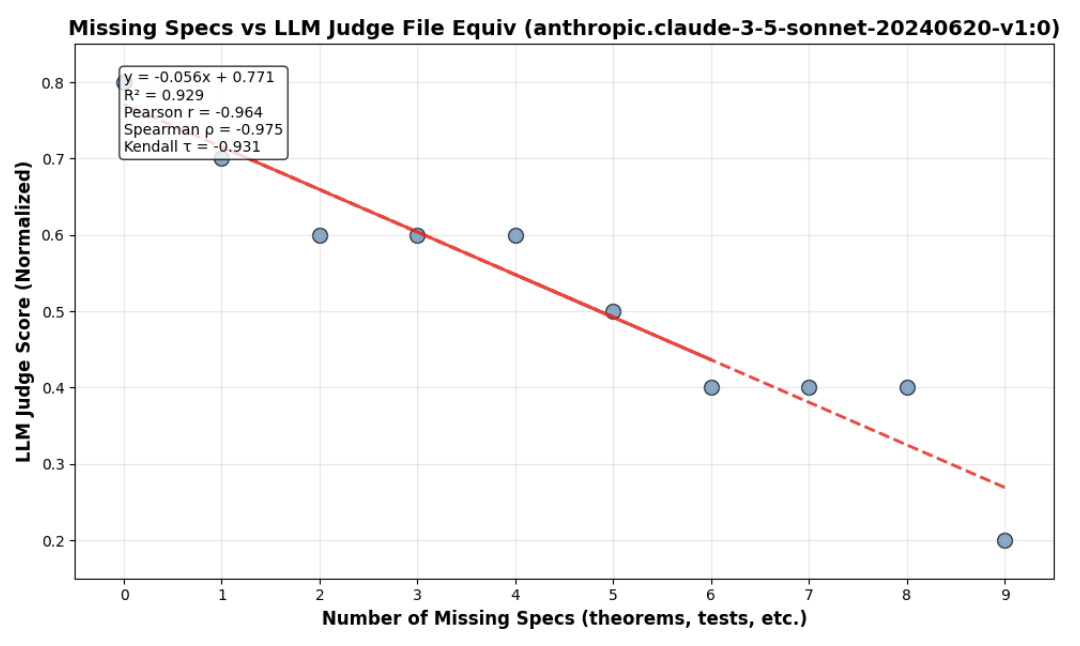
\includegraphics[width=\linewidth]{figures/3.5_specs_missing.png}
    \caption{Claude 3.5 Sonnet v1: strong monotonic decrease (\(y=-0.056x+0.771\), \(R^2=0.929\), Pearson \(r=-0.964\), Spearman \(\rho=-0.975\)).}
  \end{subfigure}\hfill
  \begin{subfigure}[t]{0.48\textwidth}
    \centering
    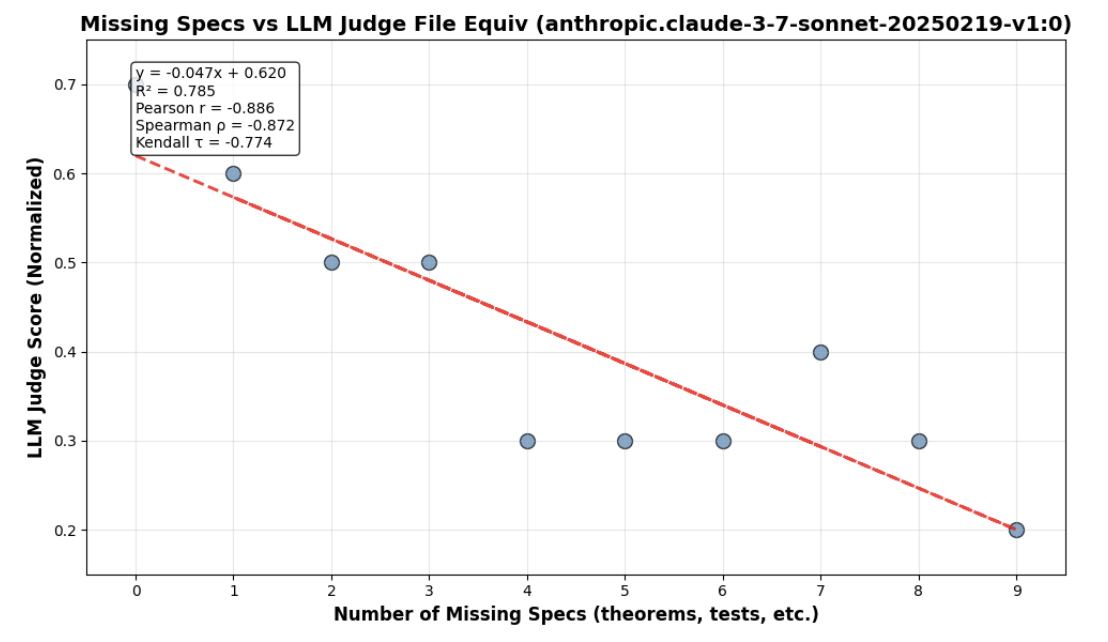
\includegraphics[width=\linewidth]{figures/3.7_specs_missing.png}
    \caption{Claude 3.7 Sonnet v1: clear negative trend with minor non-monotonicity (\(y=-0.047x+0.620\), \(R^2=0.785\), Pearson \(r=-0.886\), Spearman \(\rho=-0.872\)).}
  \end{subfigure}
  \caption{\textbf{(P3) Monotonicity w.r.t.\ missing specifications.}
    Candidate scores decrease as more theorems/tests are withheld. We retain both model variants to show robustness of the trend; 3.7’s small non-monotonicity motivated the simplified rubric used in the main results.}
  \label{fig:app-missing-specs}
\end{figure*}

\begin{figure}[t]
  \centering
  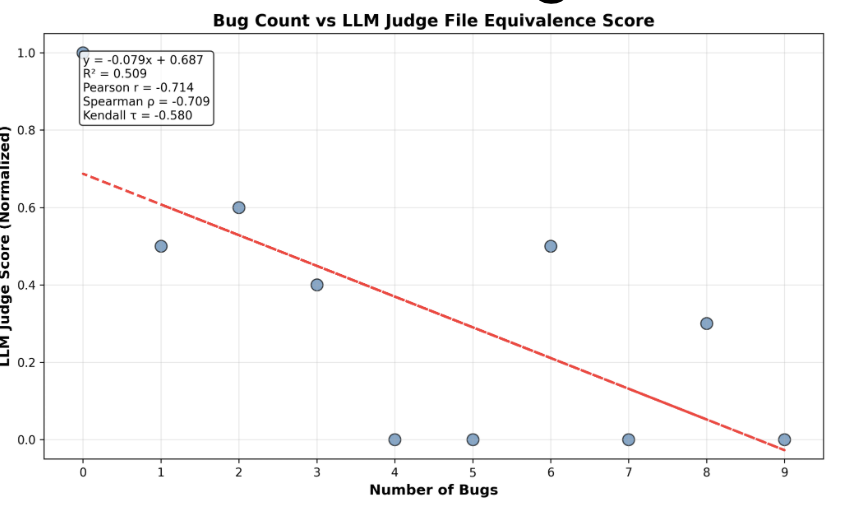
\includegraphics[width=0.85\linewidth]{figures/3.5_bugs.png}
  \caption{\textbf{(P2) Non-Monotonicity w.r.t.\ cumulative bugs (Claude 3.5 Sonnet).}
    Scores drop as more semantic bugs are injected (Pearson \(r=-0.714\), Spearman \(\rho=-0.709\), \(R^2=0.509\)); the higher noise with the initial “theorem-equivalence” prompt led us to simplify the rubric used for the final judge in the main paper.}
  \label{fig:app-bugs}
\end{figure}

\begin{figure*}[t]
  \centering
  \begin{subfigure}[t]{0.49\textwidth}
    \centering
    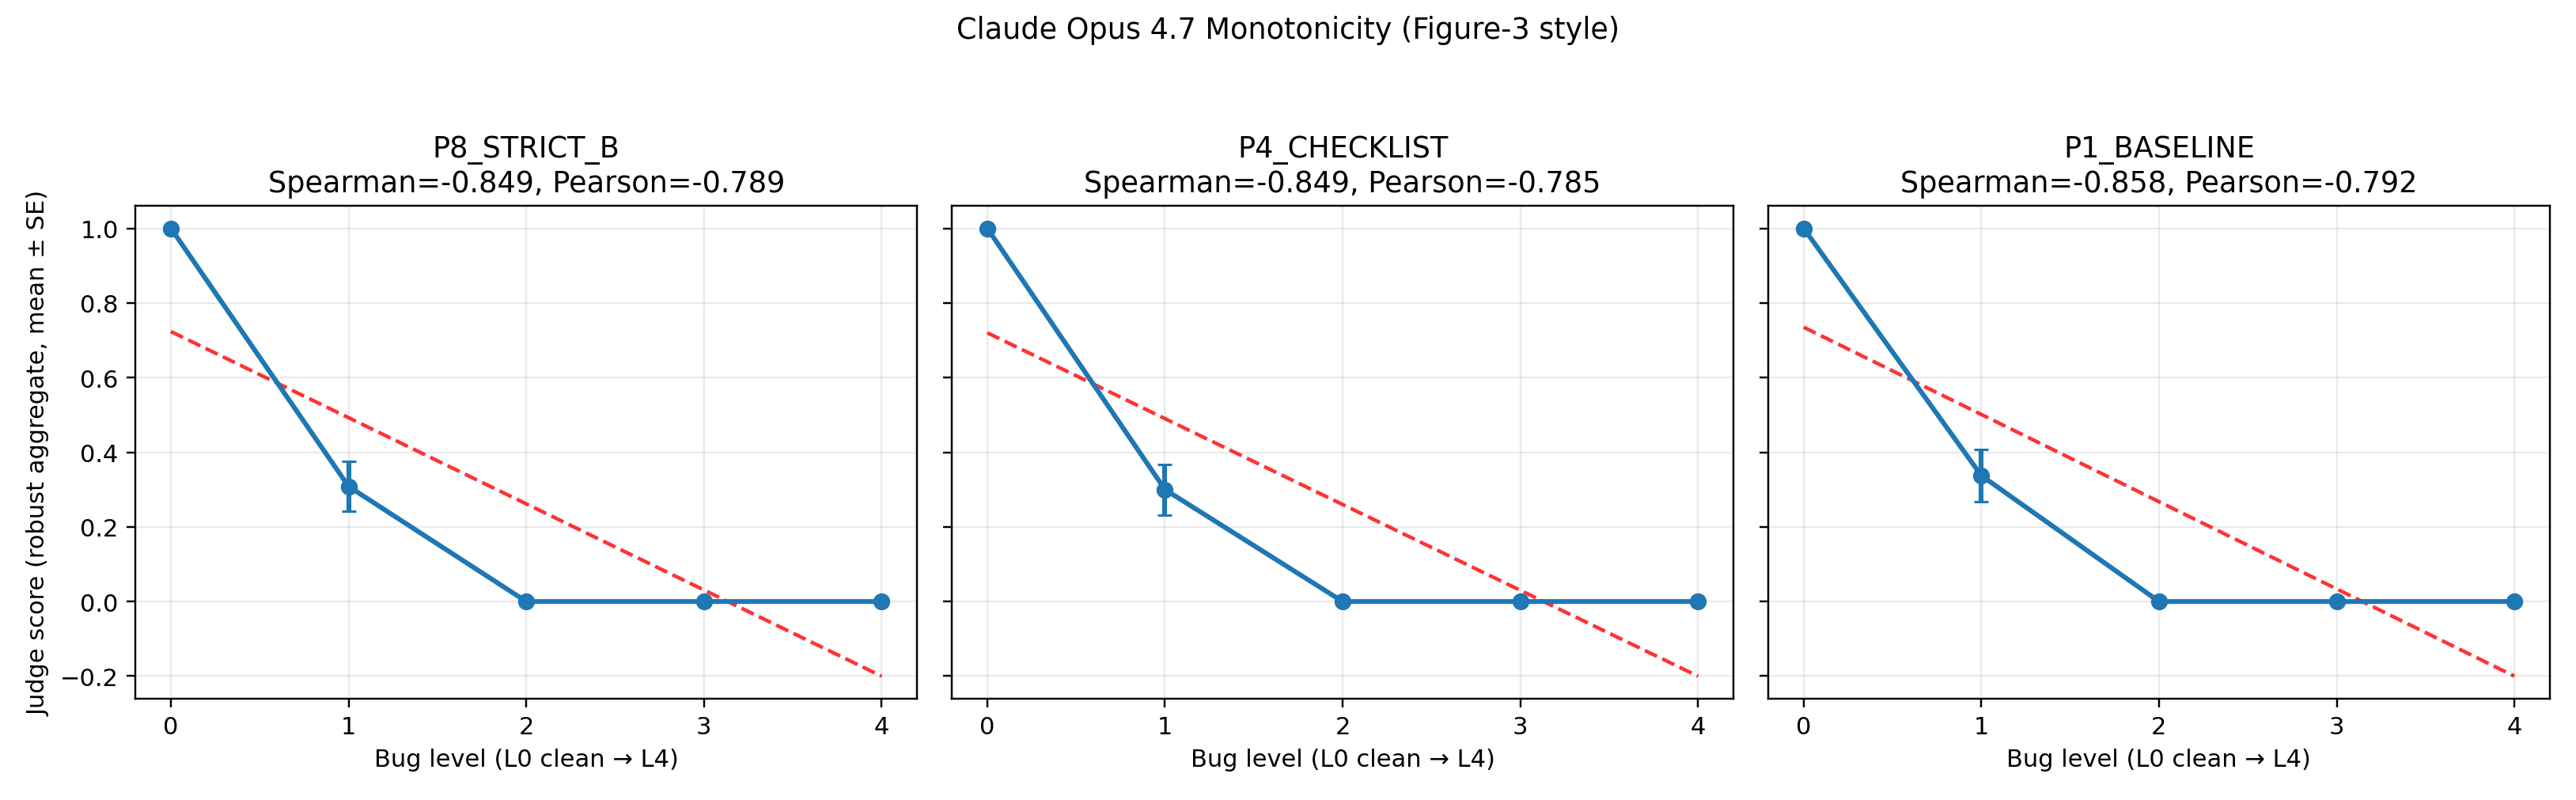
\includegraphics[width=\linewidth]{figures/fig3_style_claude_opus_monotonicity.png}
    \caption{Claude Opus 4.7 Figure-3-style monotonicity (mean \(\pm\) SE).}
  \end{subfigure}\hfill
  \begin{subfigure}[t]{0.49\textwidth}
    \centering
    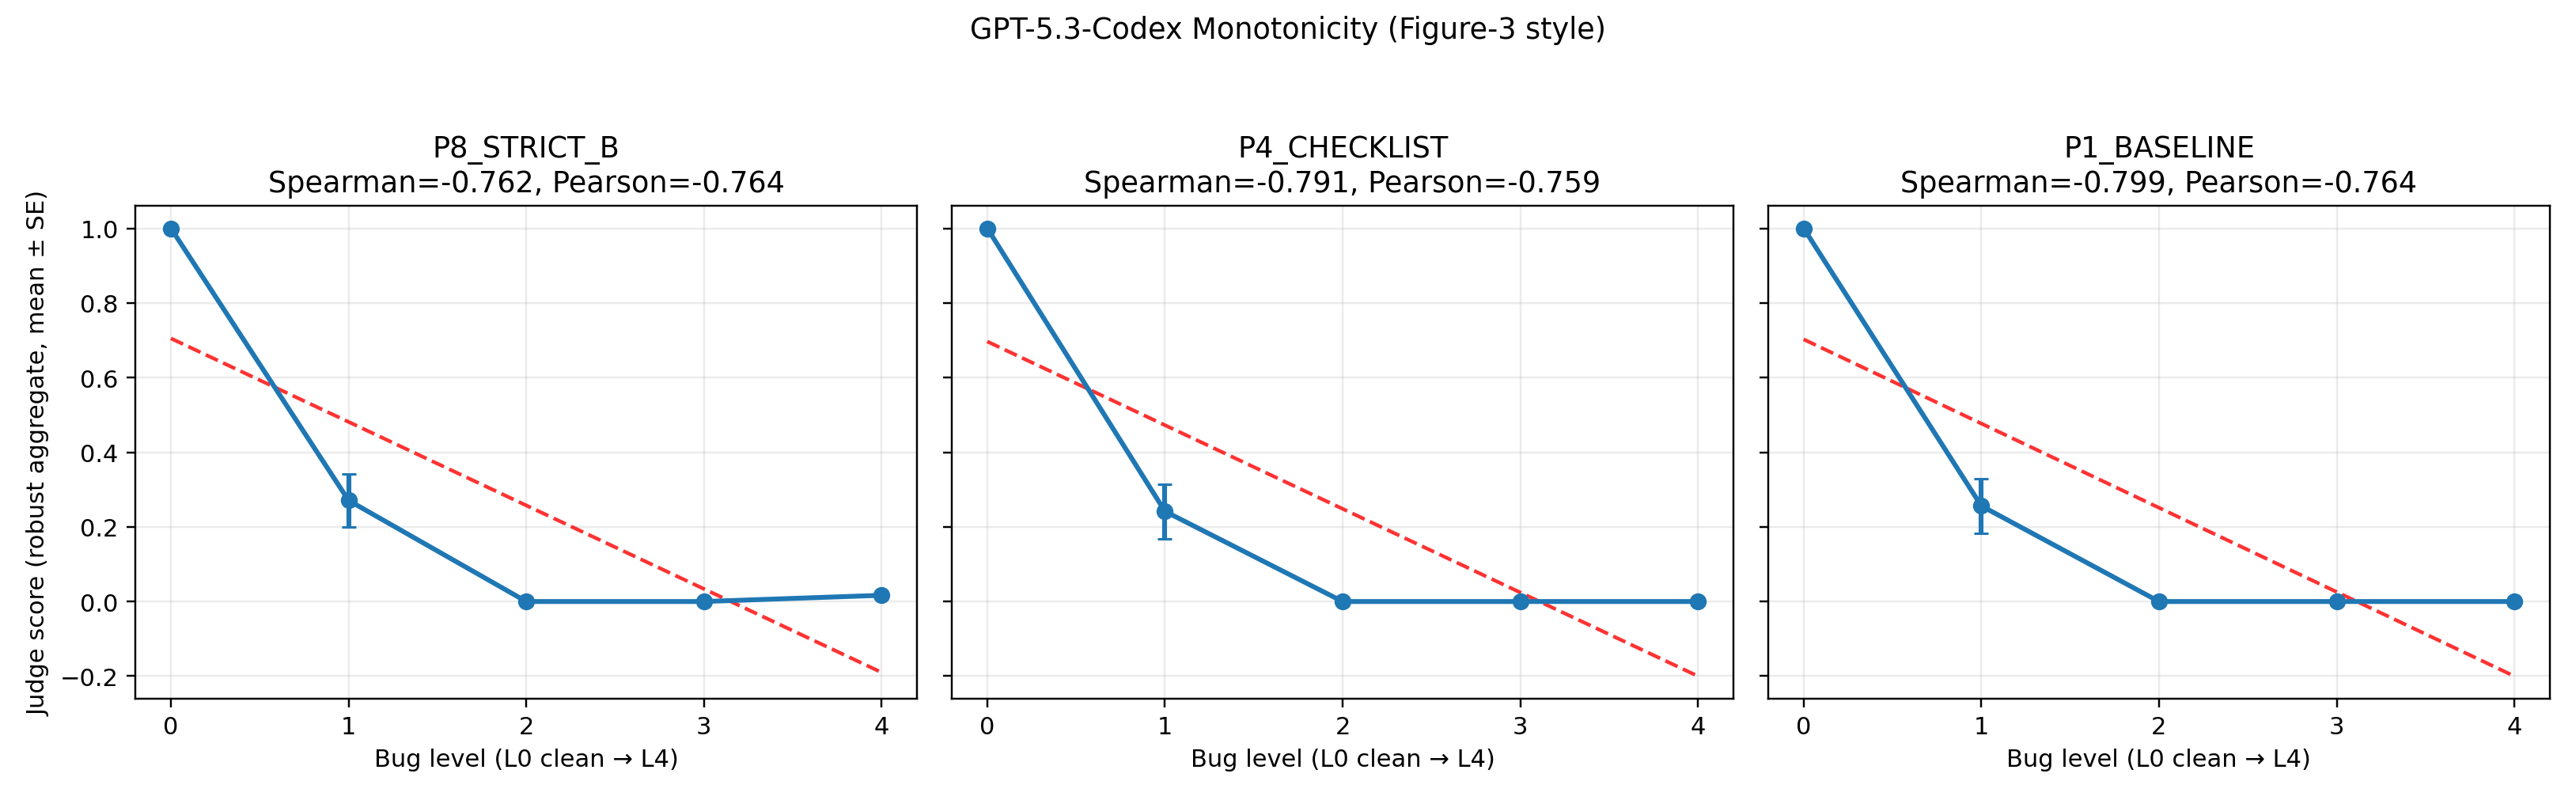
\includegraphics[width=\linewidth]{figures/fig3_style_gpt53_codex_monotonicity.png}
    \caption{GPT-5.3-Codex Figure-3-style monotonicity (mean \(\pm\) SE).}
  \end{subfigure}
  \caption{\textbf{Model-matched Figure-3-style monotonicity diagnostics.}
    Both judge families show strong monotone score degradation as bug intensity increases, under the same low-variance plotting protocol.}
  \label{fig:fig3_style_opus_codex}
\end{figure*}

\begin{figure*}[t]
  \centering
  \begin{subfigure}[t]{0.49\textwidth}
    \centering
    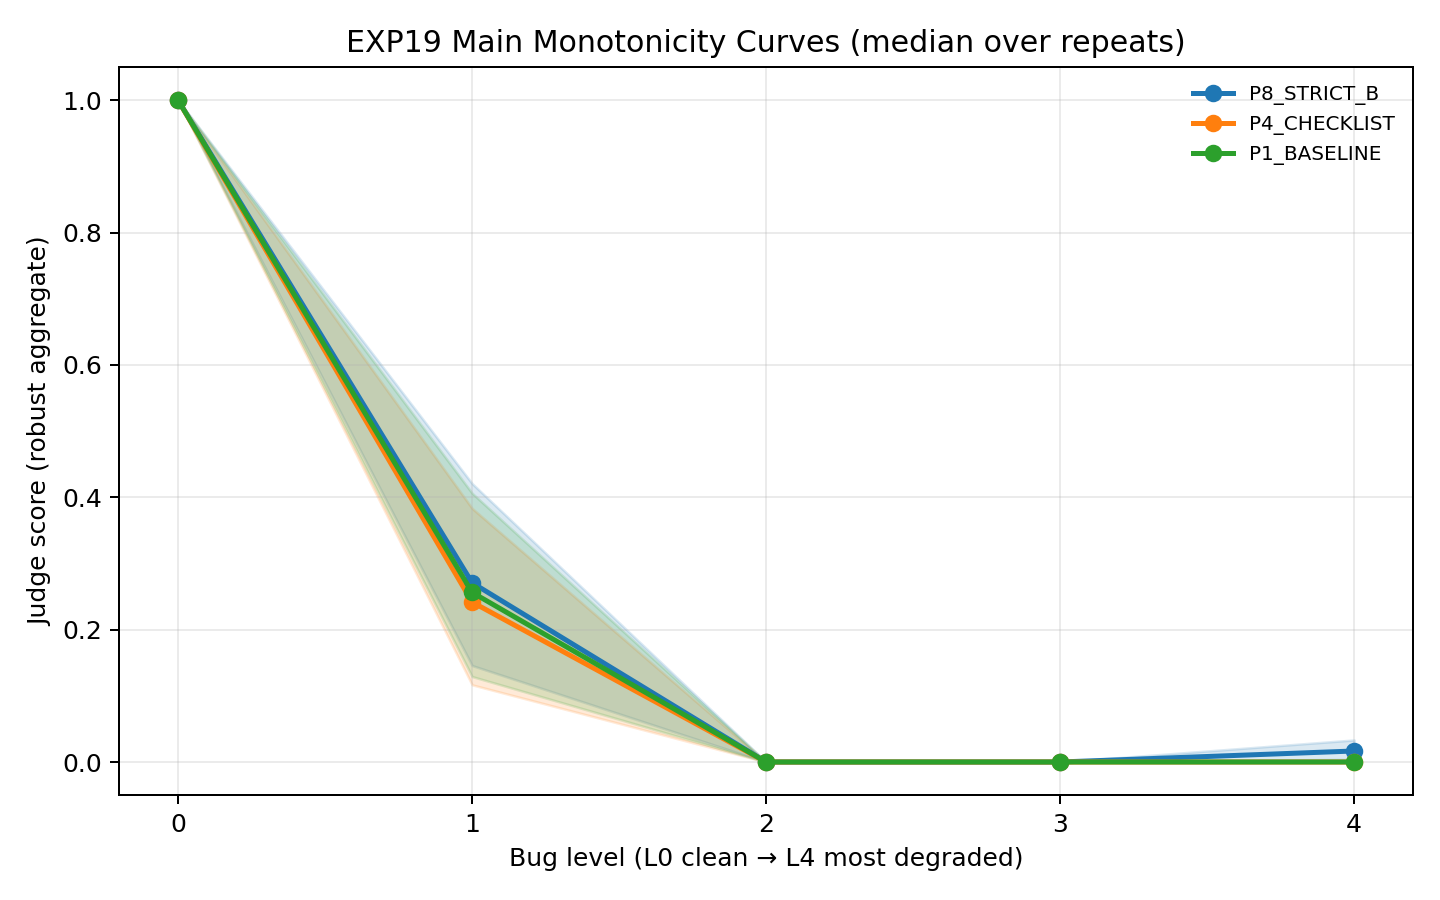
\includegraphics[width=\linewidth]{figures/fig_main_monotonicity_lowvar_codex.png}
    \caption{Codex low-variance monotonicity curves.}
  \end{subfigure}\hfill
  \begin{subfigure}[t]{0.49\textwidth}
    \centering
    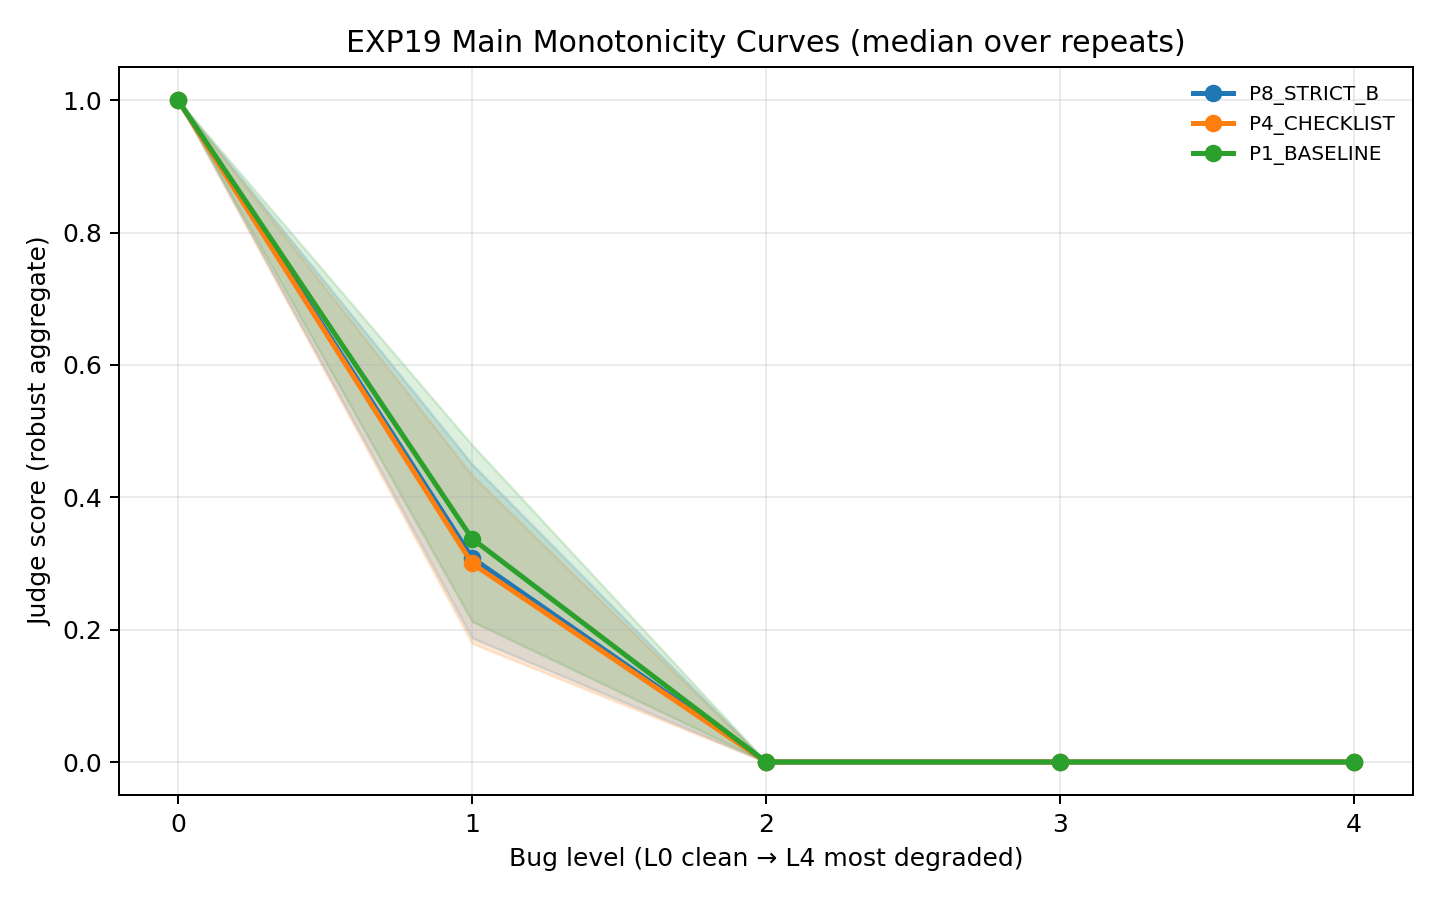
\includegraphics[width=\linewidth]{figures/fig_main_monotonicity_lowvar_opus47.png}
    \caption{Opus 4.7 low-variance monotonicity curves.}
  \end{subfigure}
  \caption{\textbf{Low-variance monotonicity trends across model families.}
    Both judge families show strong non-increasing behavior as bug intensity increases, under robust repeat aggregation.}
  \label{fig:lowvar_mono_codex_opus}
\end{figure*}

\section{Validation-Set Human Alignment Appendix}\label{app:exp16-exp17}
This appendix reports full visual diagnostics for the final robust validation-set human-alignment analyses under three label views: pass1, pass2, and avg.
We evaluate eight judge configurations spanning frontier-model prompts, weaker LLM baselines, edit-distance heuristics, and random controls.
Across this panel, \(\mathrm{TI}_{\mathrm{var}}\) strongly predicts judge-level human alignment on the calibration suite, with validation-set Spearman correlations of \(0.833\) under averaged labels, \(0.905\) under pass1 labels, and \(0.738\) under pass2 labels.
Property-level analysis shows that monotonicity under removed specifications is the strongest single predictor of human agreement, followed by monotonicity under injected bugs; identity and stability are weaker standalone signals at this scale.

\begin{figure}[t]
  \centering
  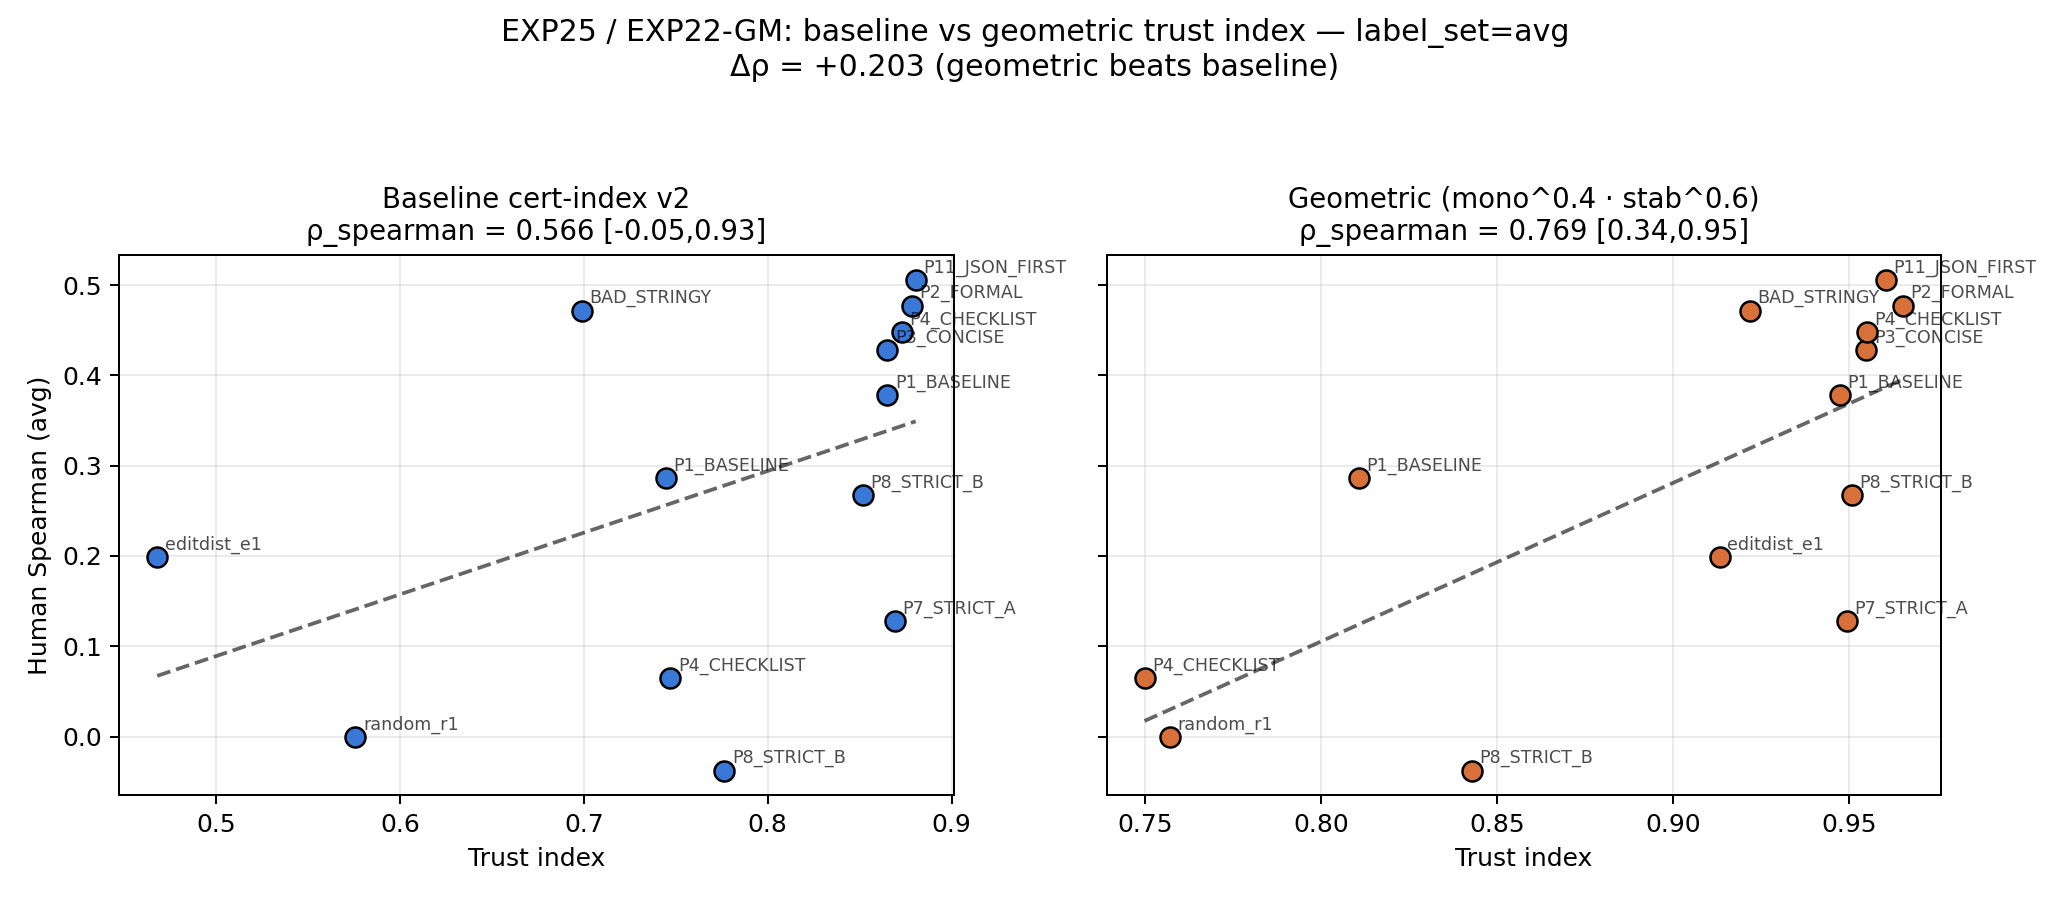
\includegraphics[width=\linewidth]{figures/fig7_trend_update_baseline_vs_geom_13judge_avg.png}
  \caption{\textbf{Expanded 13-judge panel trend (avg validation labels).}
    Geometric trust index retains strong alignment with human correlation at larger judge-panel size (\(\rho=0.769\));
    pass-specific values are pass1 \(\rho=0.764\), pass2 \(\rho=0.753\).}
  \label{fig:app-exp25-13judge}
\end{figure}

\begin{figure*}[t]
  \centering
  \begin{subfigure}[t]{0.32\textwidth}
    \centering
    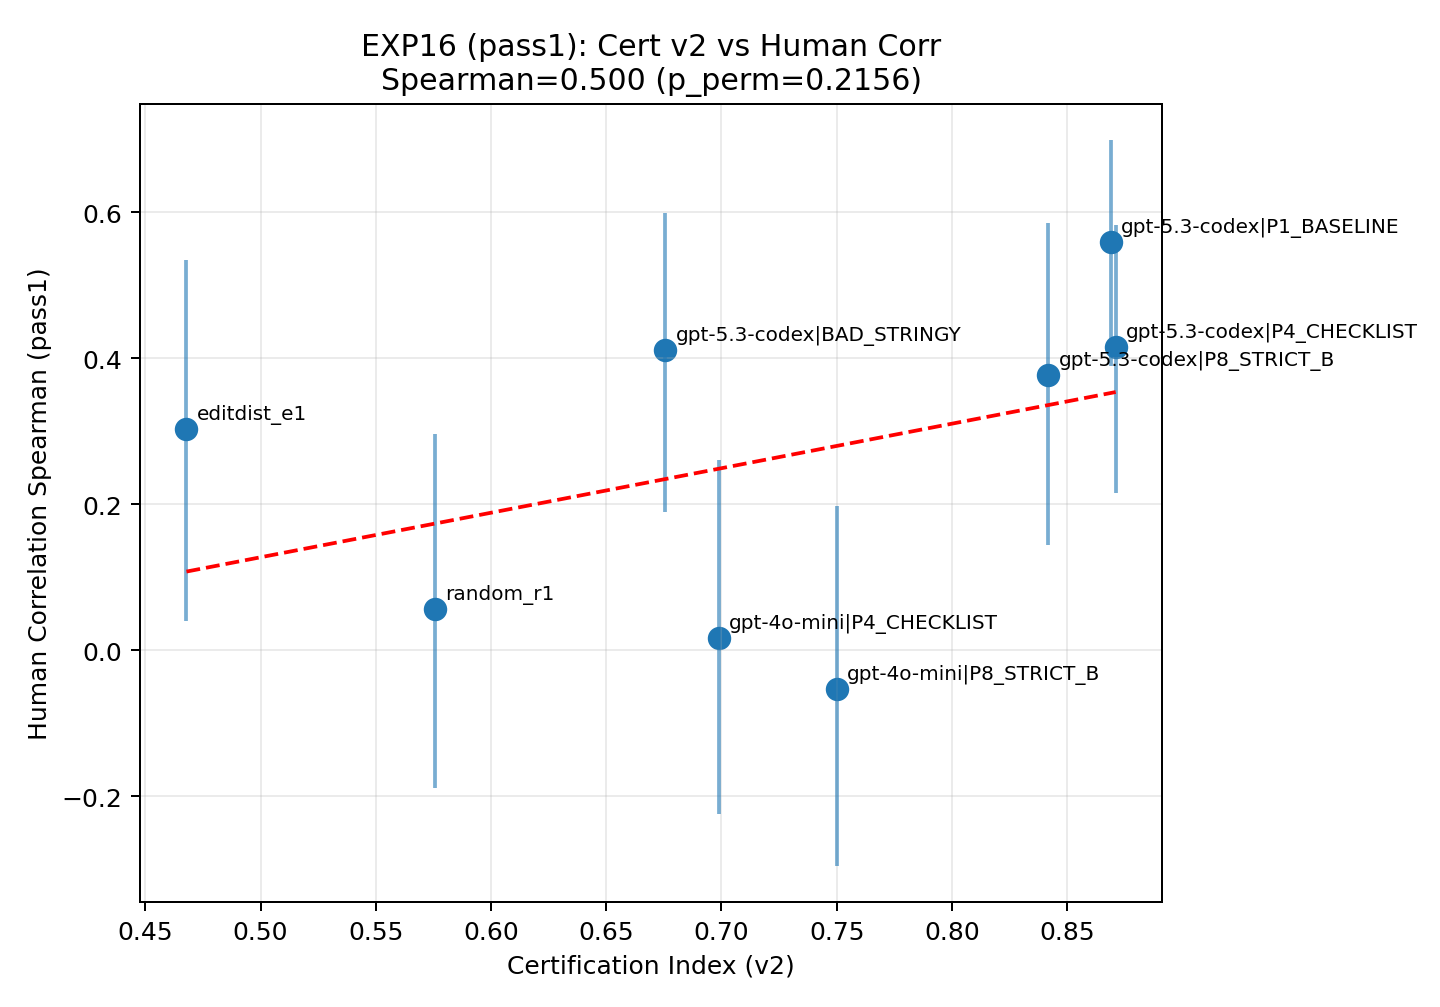
\includegraphics[width=\linewidth]{figures/exp16_final_robust/fig_cert_vs_human_scatter_pass1.png}
    \caption{Judge-level trend (pass1)}
  \end{subfigure}\hfill
  \begin{subfigure}[t]{0.32\textwidth}
    \centering
    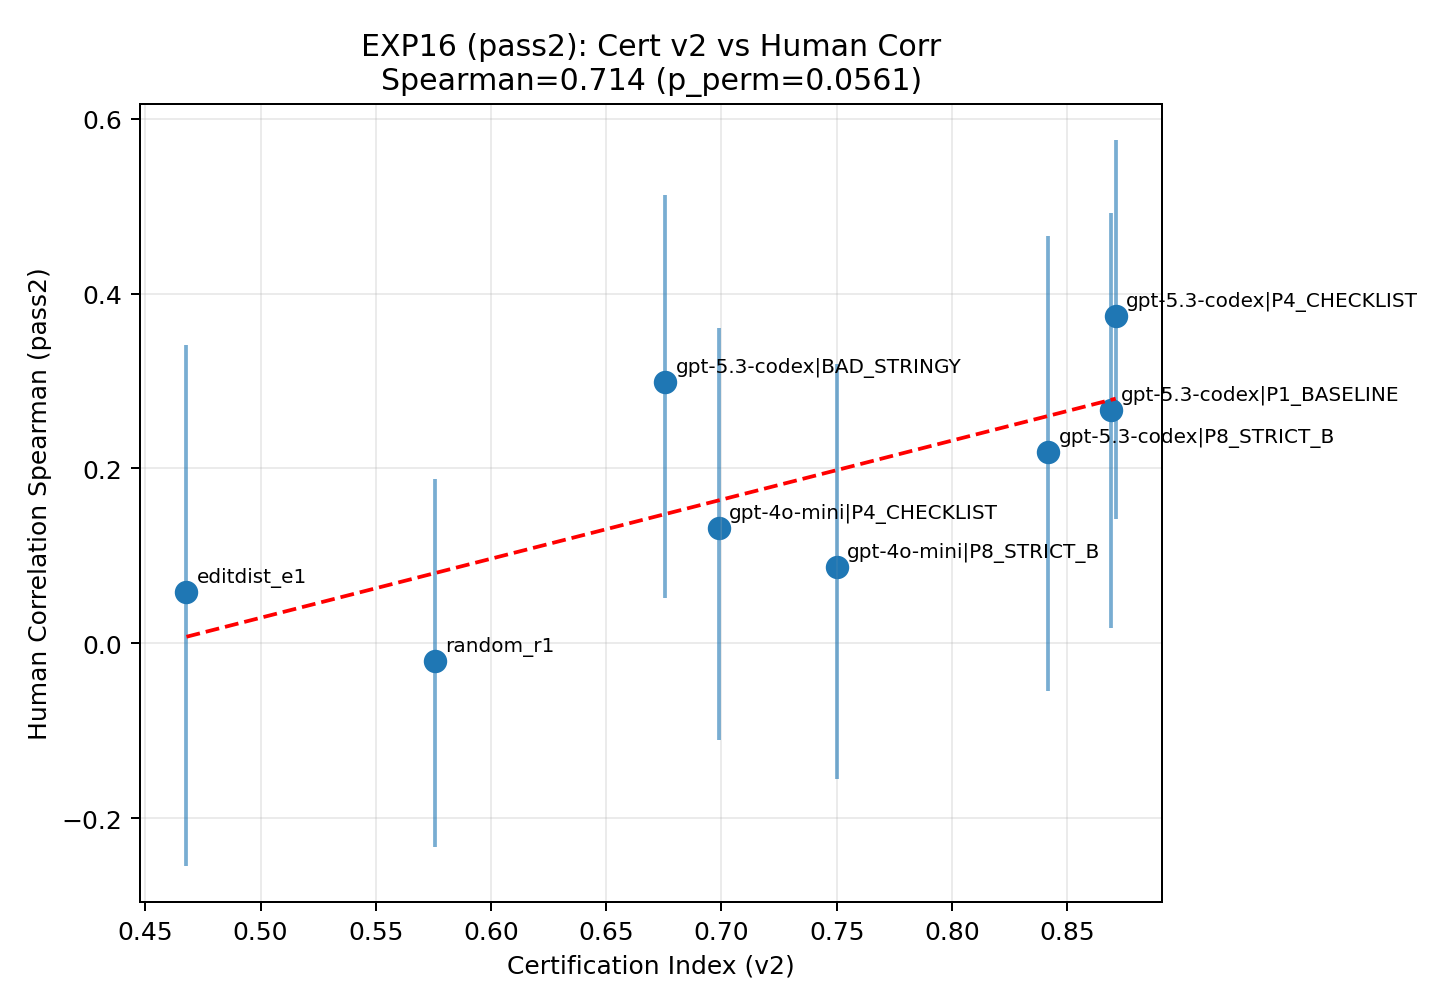
\includegraphics[width=\linewidth]{figures/exp16_final_robust/fig_cert_vs_human_scatter_pass2.png}
    \caption{Judge-level trend (pass2)}
  \end{subfigure}\hfill
  \begin{subfigure}[t]{0.32\textwidth}
    \centering
    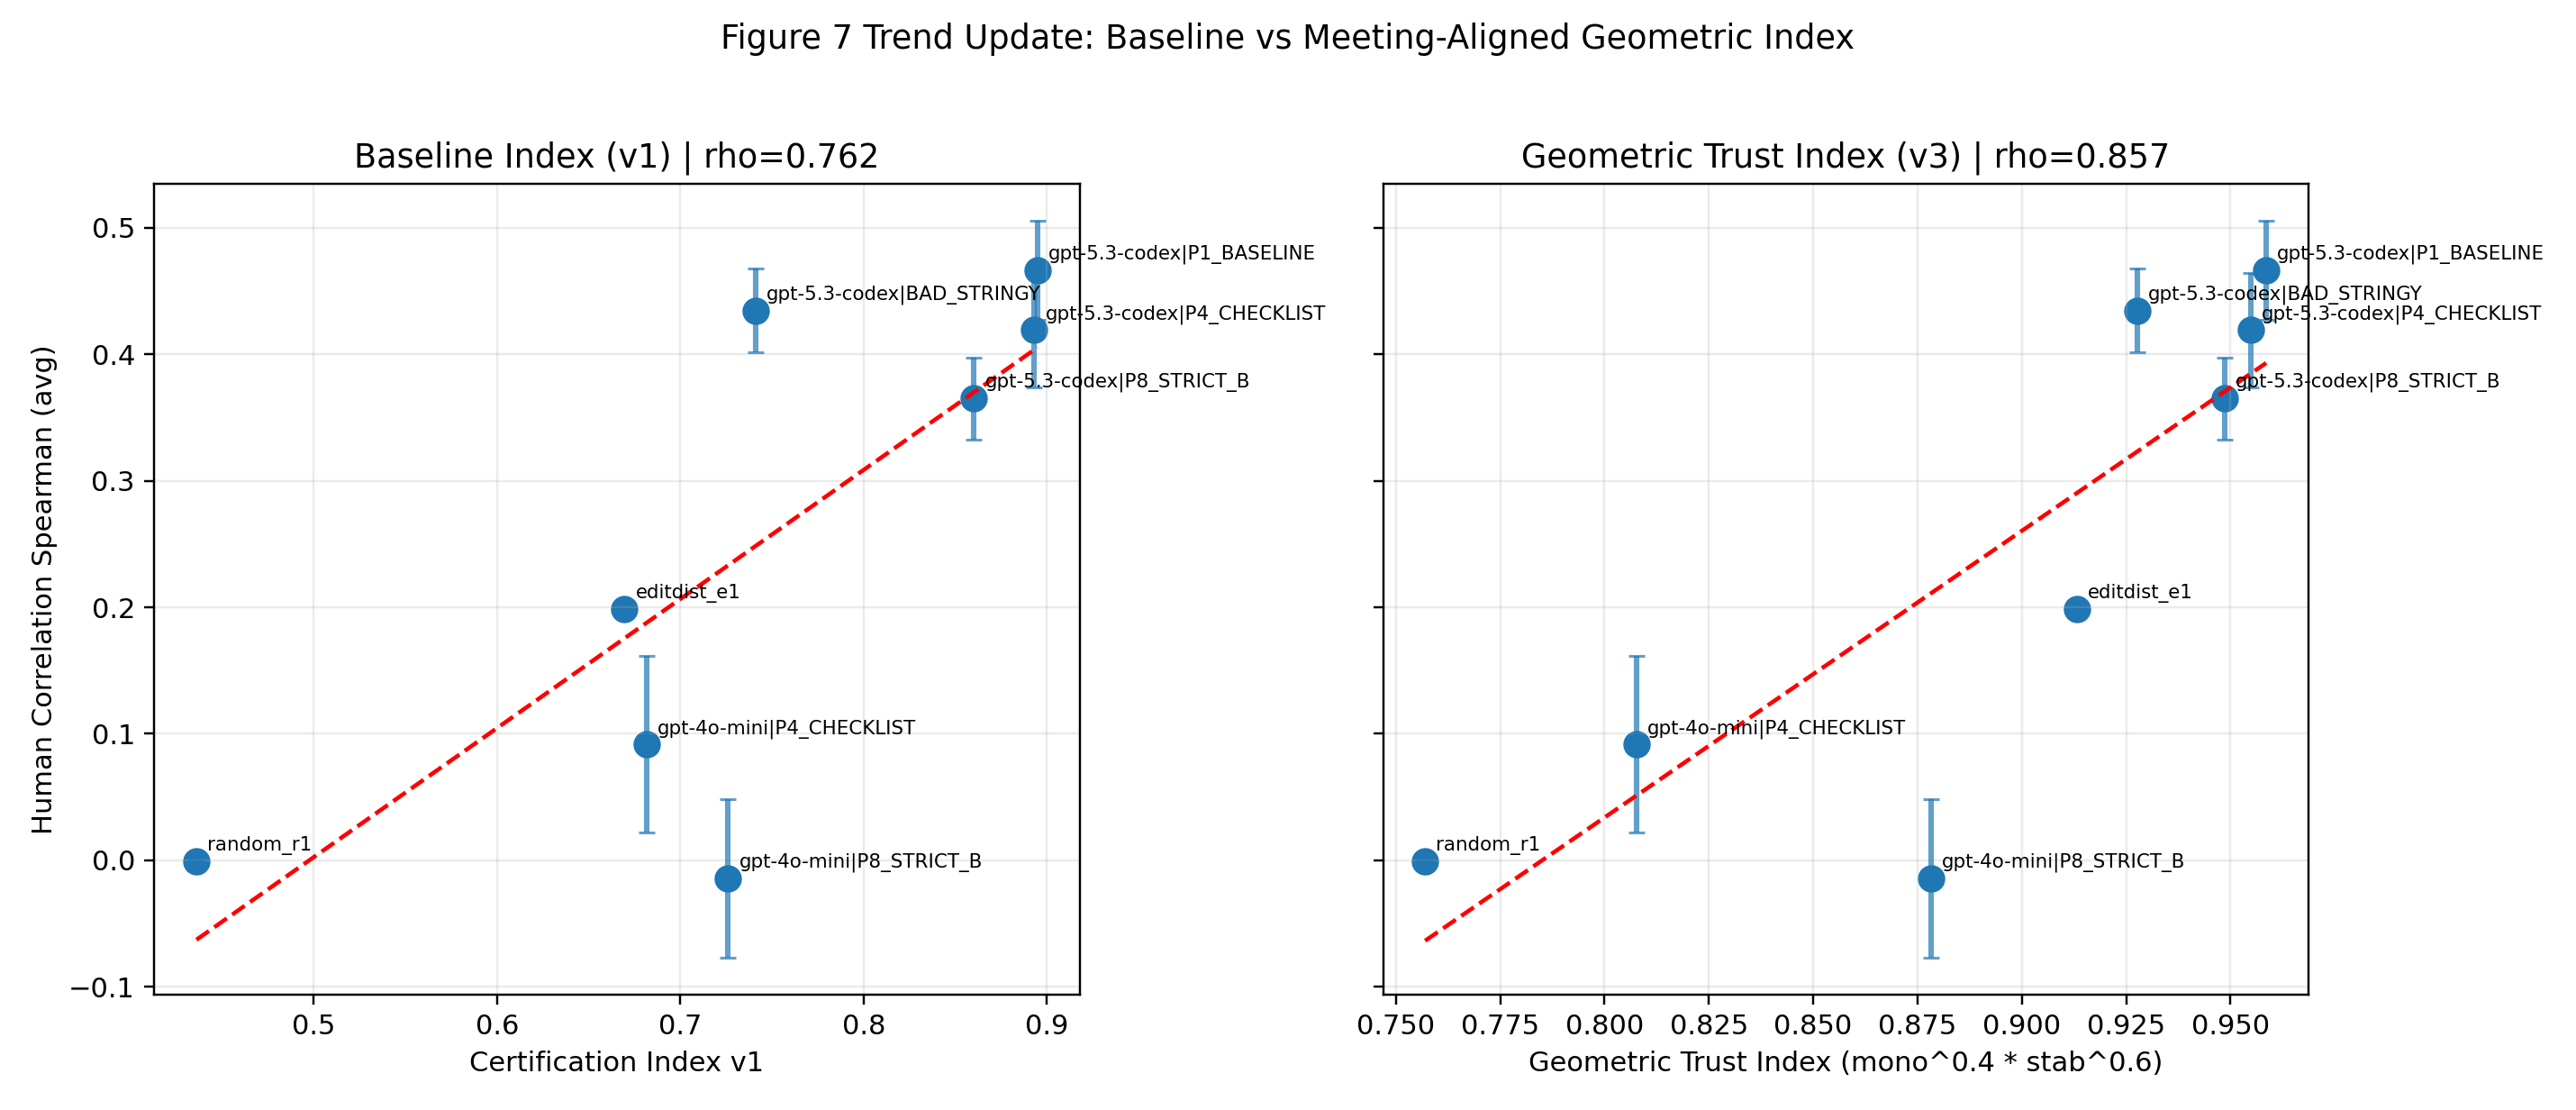
\includegraphics[width=\linewidth]{figures/exp16_final_robust/fig_cert_vs_human_scatter_avg.png}
    \caption{Judge-level trend (avg)}
  \end{subfigure}
  \caption{\textbf{Judge-level \(\mathrm{TI}_{\mathrm{var}}\)-to-human trend across validation label sets.}
  Across pass1, pass2, and averaged labels, higher certification strength is associated with stronger human agreement.}
  \label{fig:app-exp16-all}
\end{figure*}

\begin{figure*}[t]
  \centering
  \begin{subfigure}[t]{0.32\textwidth}
    \centering
    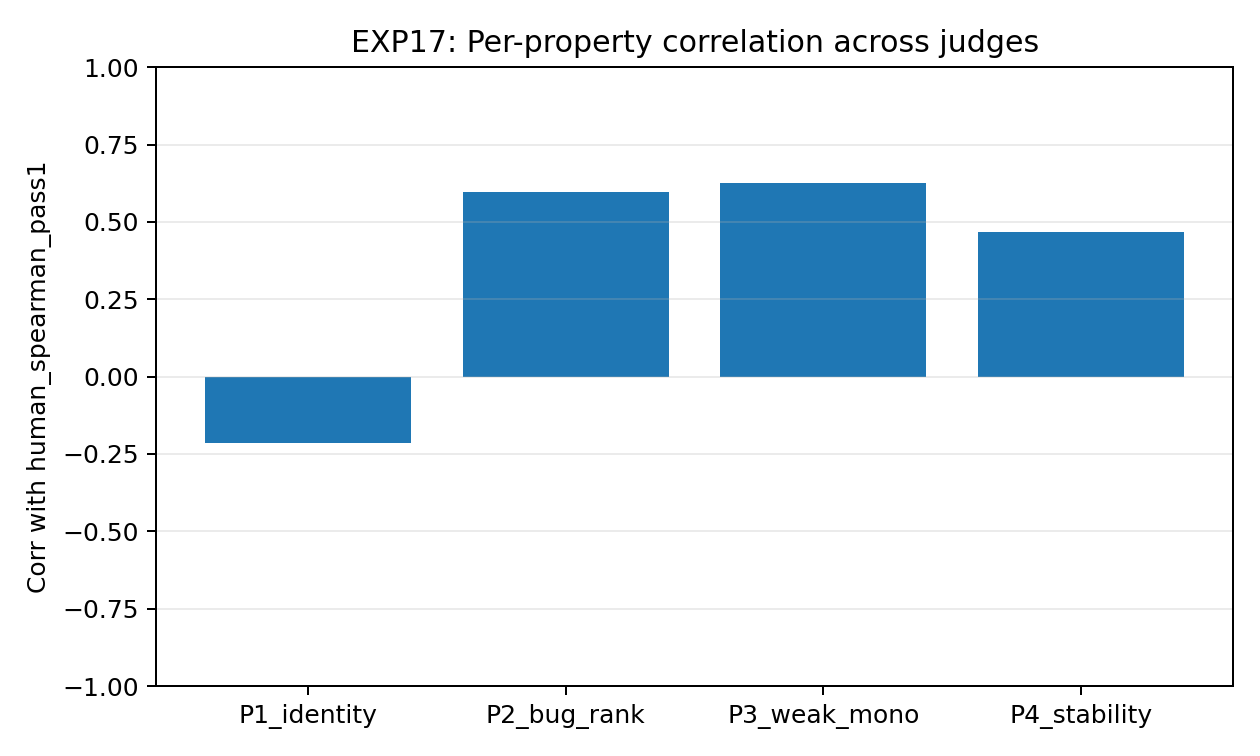
\includegraphics[width=\linewidth]{figures/exp17_final_robust/fig_property_vs_human_bars_pass1.png}
    \caption{Per-property trend (pass1)}
  \end{subfigure}\hfill
  \begin{subfigure}[t]{0.32\textwidth}
    \centering
    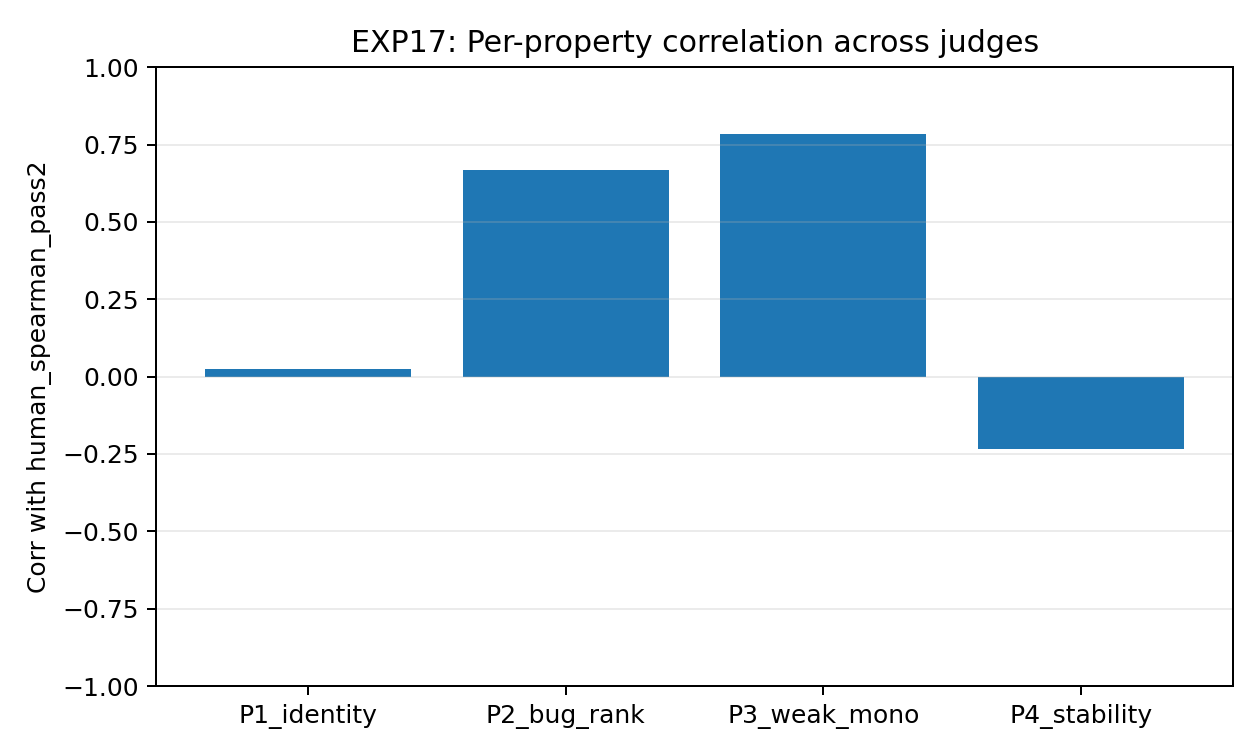
\includegraphics[width=\linewidth]{figures/exp17_final_robust/fig_property_vs_human_bars_pass2.png}
    \caption{Per-property trend (pass2)}
  \end{subfigure}\hfill
  \begin{subfigure}[t]{0.32\textwidth}
    \centering
    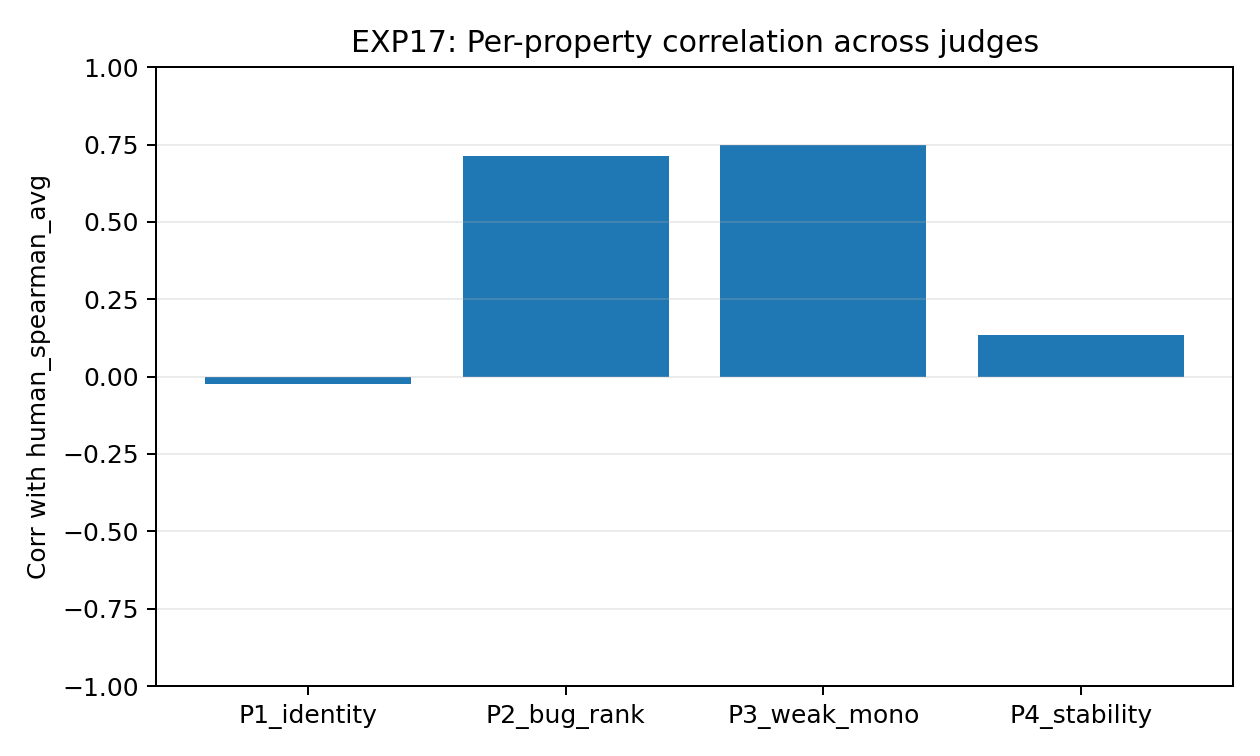
\includegraphics[width=\linewidth]{figures/exp17_final_robust/fig_property_vs_human_bars_avg.png}
    \caption{Per-property trend (avg)}
  \end{subfigure}
  \caption{\textbf{Property-wise validation-set human-alignment diagnostics.}
    P3 weak monotonicity is consistently the strongest predictor across label sets; P2 is second strongest; P1/P4 are weaker as standalone predictors at this scale.}
  \label{fig:app-exp17-all}
\end{figure*}

\begin{figure}[t]
  \centering
  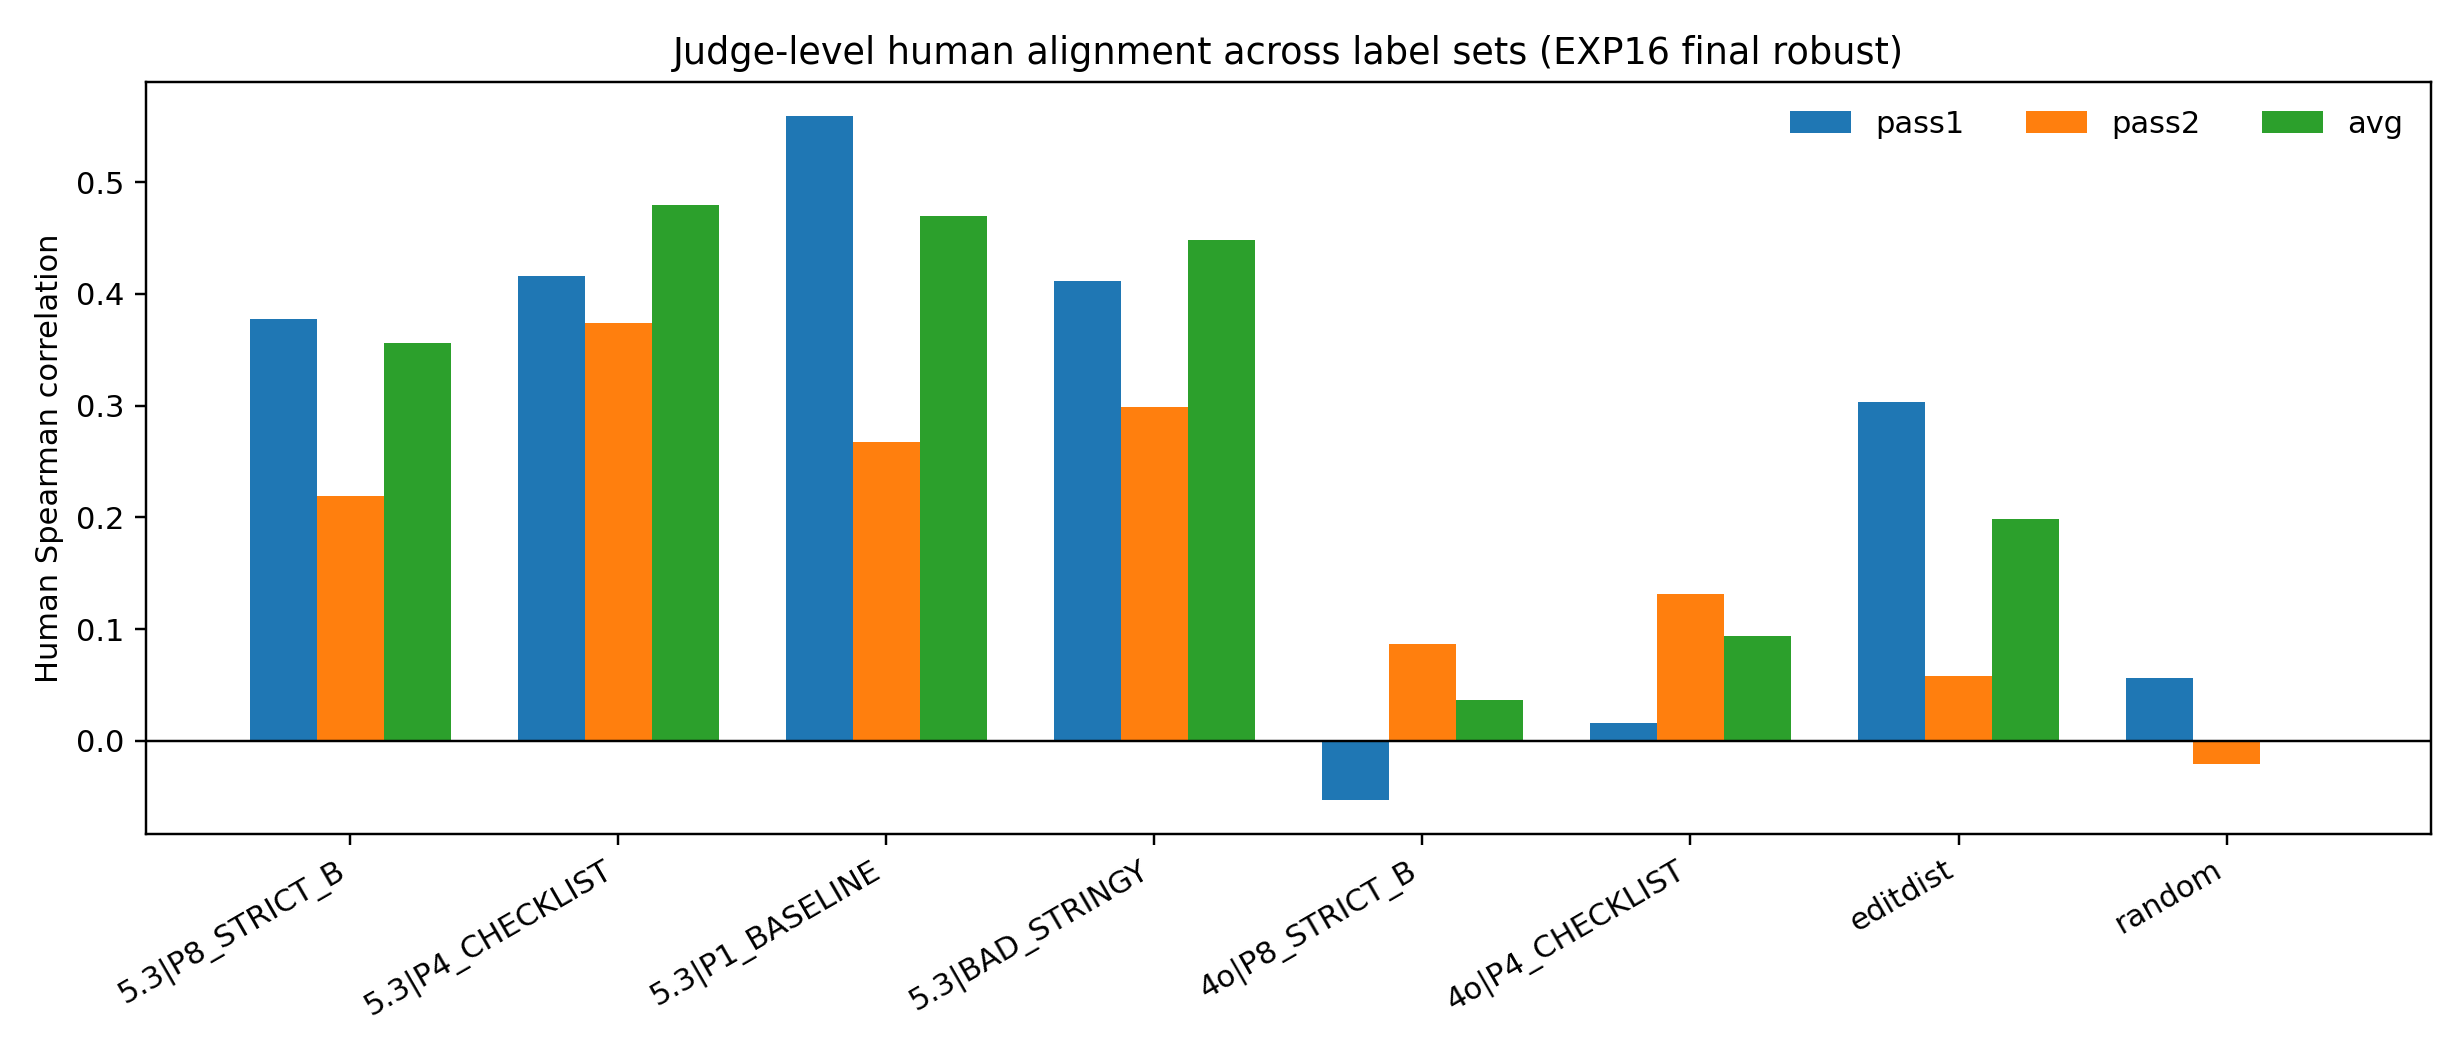
\includegraphics[width=\linewidth]{figures/exp16_final_robust/fig_human_corr_by_judge_and_labelset.png}
  \caption{\textbf{Judge-wise human alignment across label passes.} Validation-set human Spearman across pass1, pass2, and averaged labels.
    GPT-5.3-Codex variants remain above weaker baselines on most label sets; pass-to-pass variation is visible and motivates reporting all three label sets.}
  \label{fig:app-judge-labelset-bars}
\end{figure}

\subsection{Naive Codex-Style Blind Baseline}
To contextualize TI-ranked judge performance, we evaluate a naive blind baseline on the same pair set (\(n=5\) overlap), using a single-pass, surface-form-oriented Codex-style rubric without property-calibration constraints (no monotonicity/stability calibration).
The baseline tracks pass2 labels somewhat but remains substantially weaker and less consistent than the top TI-ranked judges, especially on pass1 and in absolute error.

\begin{table}[t]
  \centering
  \small
  \resizebox{\columnwidth}{!}{%
    \begin{tabular}{lcccc}
      \toprule
      \textbf{Label Set} & \(\rho_s\)                      & \(r\)                           & \(\tau\)                        & \textbf{MAE} \\
      \midrule
      pass1              & 0.171 (\(p=0.151\))             & 0.218 (\(p=0.0656\))            & 0.155 (\(p=0.144\))             & 1.049        \\
      pass2              & 0.388 (\(p=7.58\times10^{-4}\)) & 0.427 (\(p=1.87\times10^{-4}\)) & 0.343 (\(p=9.40\times10^{-4}\)) & 1.333        \\
      \bottomrule
    \end{tabular}
  }
  \caption{\textbf{Naive blind baseline vs.\ validation labels (0--5 scale).}
    \(\rho_s\): Spearman, \(r\): Pearson, \(\tau\): Kendall; MAE is absolute error on the 0--5 scale.
    This baseline is included as a sanity-check negative control and is not used for final ranking claims.}
  \label{tab:app-naive-blind-baseline}
\end{table}

\subsection{Human-Human Agreement Ceiling Context}
Validation-set judge-human Spearman values should be interpreted relative to the reliability of human labels themselves.
Across the two human annotation passes on the aligned set (\(n=75\)), inter-pass agreement is moderate (Spearman \(0.249\), Pearson \(0.375\), Kendall \(0.221\), QWK \(0.372\)).
Thus, validation-set judge-human Spearman values in the \(0.48\)--\(0.56\) range are non-trivial and should be interpreted as approaching the available annotation ceiling in this dataset rather than as ``low absolute'' values.

\begin{table}[t]
  \centering
  \small
  \begin{tabular}{@{}p{0.46\columnwidth}p{0.14\columnwidth}p{0.30\columnwidth}@{}}
    \toprule
    \textbf{Quantity}                           & \textbf{Value} & \textbf{Notes}                      \\
    \midrule
    Human-human Spearman (pass1 vs pass2)       & 0.249          & \(95\%\ \text{CI}=[-0.015, 0.489]\) \\
    Human-human Pearson (pass1 vs pass2)        & 0.375          & \(95\%\ \text{CI}=[0.076, 0.604]\)  \\
    Human-human QWK (pass1 vs pass2)            & 0.372          & \(95\%\ \text{CI}=[0.073, 0.581]\)  \\
    Human-human MAE (pass1 vs pass2)            & 0.778          & On aligned \(n=75\), 0--5 rubric    \\
    Human-human MSE (pass1 vs pass2)            & 1.139          & On aligned \(n=75\), 0--5 rubric    \\
    JS divergence (pass1 vs pass2)              & 0.081 bits     & Symmetric histogram divergence      \\
    KL\((\text{pass1}\Vert\text{pass2})\)       & 0.415 bits     & Asymmetric divergence               \\
    Best validation-set Spearman (avg labels)   & 0.480          & Best single judge on avg labels     \\
    Best validation-set Spearman (pass1 labels) & 0.559          & Best single judge on pass1 labels   \\
    \bottomrule
  \end{tabular}
  \caption{\textbf{Human-human agreement ceiling context.}
    Inter-pass human agreement is moderate, and inter-pass dispersion (MAE/divergence) is non-zero, so validation-set judge-human values near \(0.5\) are meaningful on this benchmark and should be interpreted with label-noise context.}
  \label{tab:app-human-human-ceiling}
\end{table}

\begin{figure}[t]
  \centering
  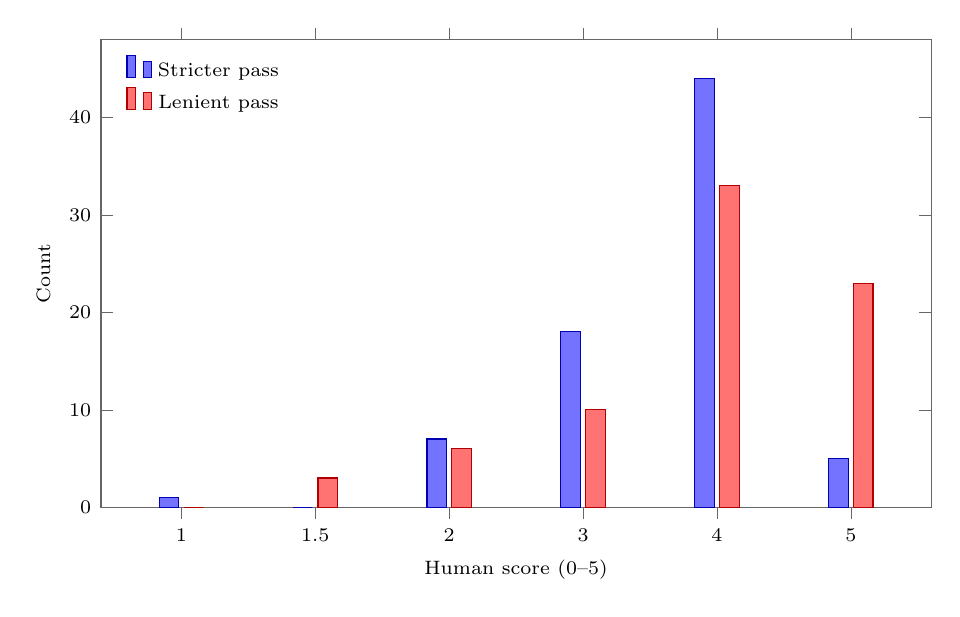
\begin{tikzpicture}
    \begin{axis}[
        width=\linewidth,
        height=0.62\linewidth,
        ybar,
        bar width=7pt,
        ymin=0,
        ymax=48,
        ylabel={Count},
        xlabel={Human score (0--5)},
        symbolic x coords={1,1.5,2,3,4,5},
        xtick=data,
        x tick label style={font=\scriptsize},
        y tick label style={font=\scriptsize},
        label style={font=\scriptsize},
        legend style={font=\scriptsize, draw=none, at={(0.02,0.98)}, anchor=north west},
        enlarge x limits=0.12,
        axis line style={black!60},
        tick style={black!60},
      ]
      \addplot+[fill=blue!55, draw=blue!70!black] coordinates {
          (1,1) (1.5,0) (2,7) (3,18) (4,44) (5,5)
        };
      \addplot+[fill=red!55, draw=red!70!black] coordinates {
          (1,0) (1.5,3) (2,6) (3,10) (4,33) (5,23)
        };
      \legend{Stricter pass,Lenient pass}
    \end{axis}
  \end{tikzpicture}
  \caption{\textbf{Human-score dispersion across passes (aligned \(n=75\), 0--5 scale).}
    Score counts are computed on the full set of \(75\) aligned candidate--gold pairs shared across both passes. The lenient pass includes three \(1.5\) scores because duplicated legacy entries for one problem were averaged before plotting. The visible distribution shift is consistent with the non-zero MAE/MSE and divergence statistics in Table~\ref{tab:app-human-human-ceiling}.}
  \label{fig:app-human-pass-hist}
\end{figure}

\subsection{Cross-Model Validation Status (Full vs Preliminary)}
To avoid over-claiming, we separate full-scale cross-model regressions (\(n{=}8\) judge tuples on the \(\sim\!\!72\)–\(75\) overlapping aligned rows for each labeling view) from narrower exploratory protocol plots.
\textbf{Anthropic Claude Opus (4.x)} \(\mathrm{TI}_{\mathrm{var}}\) vs.\ validation human Spearman is a full-panel run of the same form as GPT-5.3-Codex and Qwen3-Coder in Figure~\ref{fig:tivar_cross_model_avg}: eight judge configurations (four Opus \(\times\) prompts plus cross-family \(\texttt{gpt-4o-mini}\)\(\times\)two prompts plus edit/random controls), repeated-judge aggregation, identical label sets.

Early \textbf{Claude 3.x Sonnet} scatterplots reported in Appendix~\ref{app:judge-cert} were small-file protocol iterations used mainly to stabilize prompts and ladders; those plots illustrate qualitative monotonic behavior but are \emph{not} the statistic behind Table~\ref{tab:tivar_cross_model_results}.

\begin{table}[t]
  \centering
  \scriptsize
  \setlength{\tabcolsep}{3pt}%
  \begin{tabular}{@{}>{\raggedright\arraybackslash}p{0.52\linewidth}
    >{\centering\arraybackslash}p{0.09\linewidth}
    >{\centering\arraybackslash}p{0.07\linewidth}
    >{\raggedright\arraybackslash}p{0.22\linewidth}@{}}
    \toprule
    \textbf{Judge setup}                 &
    \textbf{Scale}                       &
    \textbf{Main?}                       &
    \textbf{Role}                                                                     \\
    \midrule
    GPT-5.3-Codex prompts (P8/P4/P1)     & \(n{=}8\) & Yes & Primary judges           \\
    GPT-5.3-Codex BAD\_STRINGY           & \(n{=}8\) & Yes & Same-model stress        \\
    Qwen3-Coder prompts                  & \(n{=}8\) & Yes & Open-weights             \\
    Qwen3-Coder BAD\_STRINGY             & \(n{=}8\) & Yes & Open-weights stress      \\
    Claude Opus 4.x + controls           & \(n{=}8\) & Yes & Third cross-model family \\
    GPT-4o-mini prompts                  & \(n{=}8\) & Yes & Lightweight baseline     \\
    Edit-distance + random               & \(n{=}8\) & Yes & Non-LLM controls         \\
    Claude 3 Sonnet (narrow App.\ slice) & Small     & No  & Prompt diagnostics       \\
    \bottomrule
  \end{tabular}
  \caption{\textbf{Cross-model validation status.}
  Main \(\mathrm{TI}_{\mathrm{var}}\) claims use full eight-configuration panels on overlapping human-aligned rows; Sonnet exploratory figures are withheld from headline statistics.}
  \label{tab:app-cross-model-status}
\end{table}

\subsection{Leanstral Negative-Control Reaggregation (AM/GM/Variance-Aware)}
To stress-test whether index choice alone can ``rescue'' a weak judge family, we re-aggregate the same Leanstral judge outputs under three indices:
\[
  \mathrm{AM}=\text{cert\_index\_v2}
  \qquad \text{(arithmetic baseline)}
\]
\[
  \mathrm{GM}=\mathrm{mono}^{0.4}\cdot \mathrm{stab}^{0.6}
\]
\[
  \begin{aligned}
    \mathrm{TI}_{\mathrm{var}}
    ={} & \exp\!\Big(
    \tfrac{1}{3}\log C_f
    + \tfrac{1}{3}\log(1-\widetilde{\mathrm{VarCorr}}) \\
        & \qquad\quad
    + \tfrac{1}{3}\log(1-\widetilde{\mathrm{VarScore}})
    \Big)
  \end{aligned}
\]
where \(C_f\) is the aggregated P1--P4 quality term, and \(\widetilde{\mathrm{VarCorr}},\widetilde{\mathrm{VarScore}}\) are normalized variance penalties (lower is better before \(1-\cdot\)).
We report Spearman between index score and validation-set human Spearman across judges.

\subsection{Index Definitions}\label{app:index-definitions}
For reference, the simple arithmetic baselines in the main text are
\[
  v1 = 0.30\,\text{ident} + 0.30\,\text{mono\_rank} + 0.25\,\text{weak} + 0.15\,\text{stab},
\]
\[
  \begin{aligned}
    v2 ={} & 0.20\,\text{ident} + 0.20\,\text{mono\_rank} + 0.15\,\text{weak} \\
           & + 0.10\,\text{stab} + 0.20\,\text{anti} + 0.15\,\text{subtle},
  \end{aligned}
\]
where \(\text{mono\_rank}=(1-\rho_{\text{bug}})/2\) rescales bug-ladder Spearman so that larger is better, and \(\text{stab}=1-\text{flip\_rate}\).

For the variance-aware index, the quality term is
\[
  C_f = \left(\text{ident}\cdot\text{mono\_rank}\cdot\text{weak}\cdot\text{stab}\right)^{1/4},
\]
so the variance-aware index combines all four property scores before applying the variance penalties.

\begin{table}[t]
  \centering
  \small
  \resizebox{\columnwidth}{!}{%
    \begin{tabular}{lccc}
      \toprule
      \textbf{Label Set} & \textbf{AM (v2)} & \textbf{GM} & \textbf{Variance-Aware \(\mathrm{TI}_{\mathrm{var}}\)} \\
      \midrule
      val (pass1)        & -0.5952          & -0.1429     & -0.1190                                                \\
      test (pass2)       & -0.1905          & -0.2619     & -0.0476                                                \\
      avg                & -0.4286          & -0.2143     & -0.0952                                                \\
      \bottomrule
    \end{tabular}
  }
  \caption{\textbf{Leanstral remains low-alignment under multiple index constructions.}
    Re-aggregation improves over the arithmetic baseline in some splits, but all three settings remain near-zero or negative.
    This suggests the bottleneck is likely the underlying judge behavior for this ranking task (human-preference alignment), not only index form.
    One plausible hypothesis is that Leanstral is stronger for Lean proof editing/generation than for calibrated pairwise judging under this rubric; we treat this as a testable conjecture, not a final causal claim.}
  \label{tab:app-leanstral-index-reagg}
\end{table}

\subsection{Failure Modes Found by Certification (Not Hidden)}
The certification framework is useful precisely because it identifies failures:
\textbf{(i) alpha-renaming sensitivity} is the dominant identity/invariance gap,
and \textbf{(ii) local bug-ladder reversals} occur despite overall negative monotone trends.
We therefore report both strengths and weaknesses, and include alpha-ablation diagnostics.
On trend-v1 Spearman (TI \(\rightarrow\) validation-set human Spearman), excluding alpha variants changes
pass1 \(0.810\rightarrow0.690\), pass2 \(0.810\rightarrow0.714\), avg \(0.881\rightarrow0.786\),
showing that alpha cases materially affect measured robustness.

\subsection{Newest Results (Latest Rerun at Appendix Bottom)}
To reduce judge-call noise, we reran the multi-judge validation trend with higher repeats and robust repeat aggregation:
\texttt{JUDGE\_REPEATS=9 REPEAT\_AGG=median BOOTSTRAP\_ITERS=10000 PERM\_ITERS=20000}.
This run writes to \texttt{results\_exp16\_final\_robust\_r9\_median}.

\begin{table}[t]
  \centering
  \small
  \resizebox{\columnwidth}{!}{%
    \begin{tabular}{lcc}
      \toprule
      \textbf{Label Set} & \textbf{v1 Spearman}                             & \textbf{v2 Spearman}                             \\
      \midrule
      pass1              & \(0.762\) (\(p=0.0372\), CI \([-0.139, 1.000]\)) & \(0.524\) (\(p=0.1959\), CI \([-0.400, 0.975]\)) \\
      pass2              & \(0.810\) (\(p=0.0222\), CI \([0.291, 1.000]\))  & \(0.571\) (\(p=0.1477\), CI \([-0.231, 0.975]\)) \\
      avg                & \(0.762\) (\(p=0.0402\), CI \([0.103, 1.000]\))  & \(0.476\) (\(p=0.2426\), CI \([-0.425, 1.000]\)) \\
      \bottomrule
    \end{tabular}
  }
  \caption{\textbf{Latest rerun (R9 + median aggregation).}
    Increasing repeats and using median aggregation preserves the v1 trend signal while v2 remains more sensitive at this \(n_\text{judges}=8\) scale.}
  \label{tab:app-latest-r9-median}
\end{table}

We also generated a low-variance replot package from the same detail rows (\texttt{results\_exp19\_low\_variance\_replot}): a cleaner main monotonicity curve for core judges plus separate failure-mode plots for alpha sensitivity and local bug reversals.
Reversal rates in this package are: GPT-5.3 P4/P1 \(=0.00\), GPT-5.3 P8 \(=0.167\), BAD\_STRINGY \(=0.833\), GPT-4o variants \(=0.667\)--\(0.750\), edit-distance/random \(=1.00\).

\begin{figure*}[t]
  \centering
  \begin{subfigure}[t]{0.48\textwidth}
    \centering
    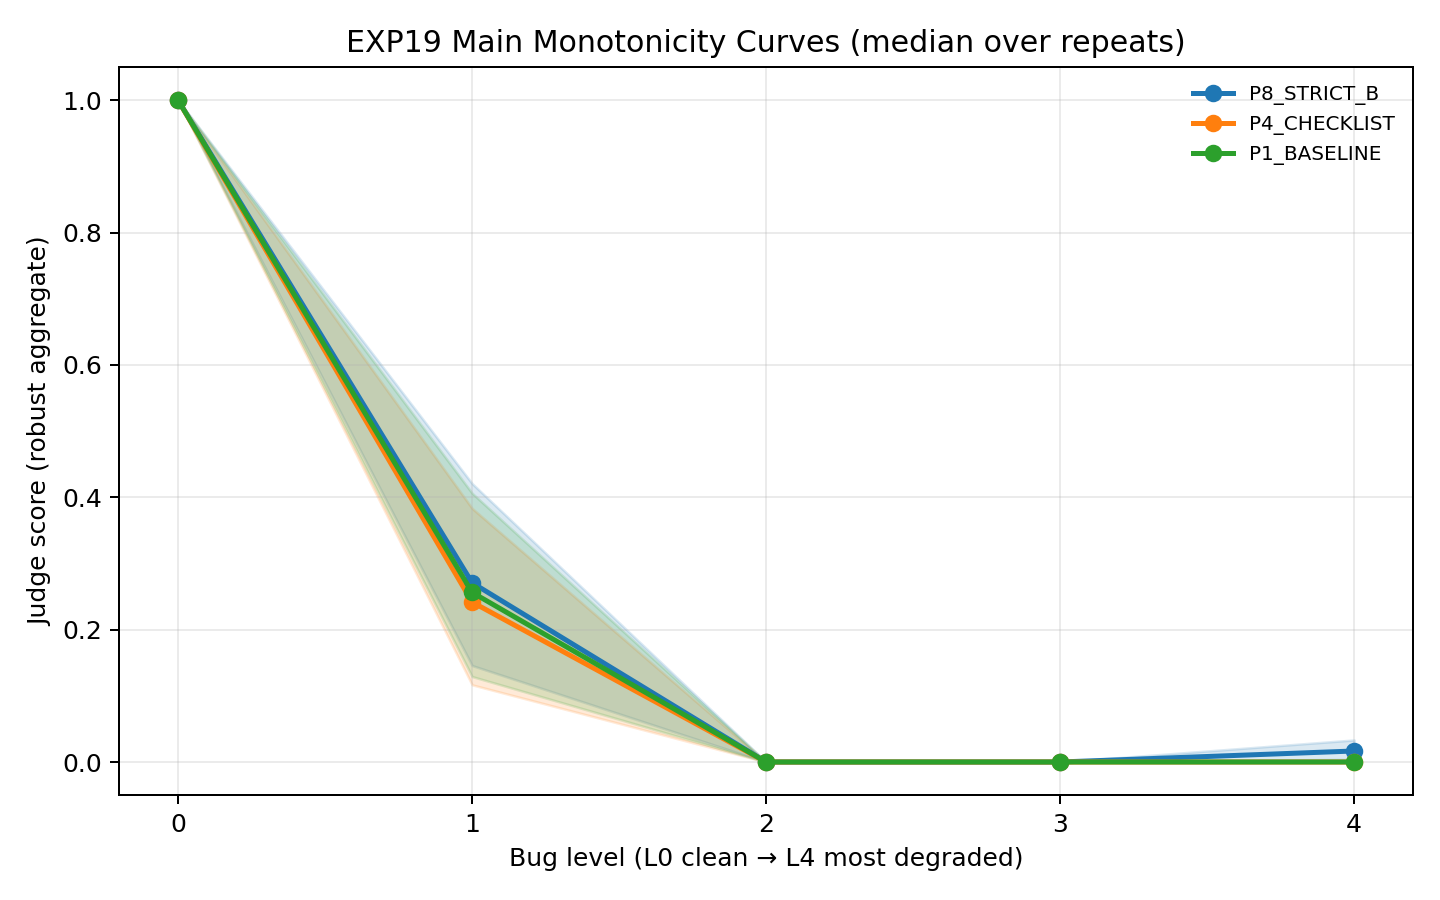
\includegraphics[width=\linewidth]{figures/fig_main_monotonicity_lowvar_exp19.png}
    \caption{Main low-variance monotonicity curves (core GPT-5.3 judges, robust repeat aggregation).}
    \label{fig:app-exp19-main-lowvar}
  \end{subfigure}\hfill
  \begin{subfigure}[t]{0.48\textwidth}
    \centering
    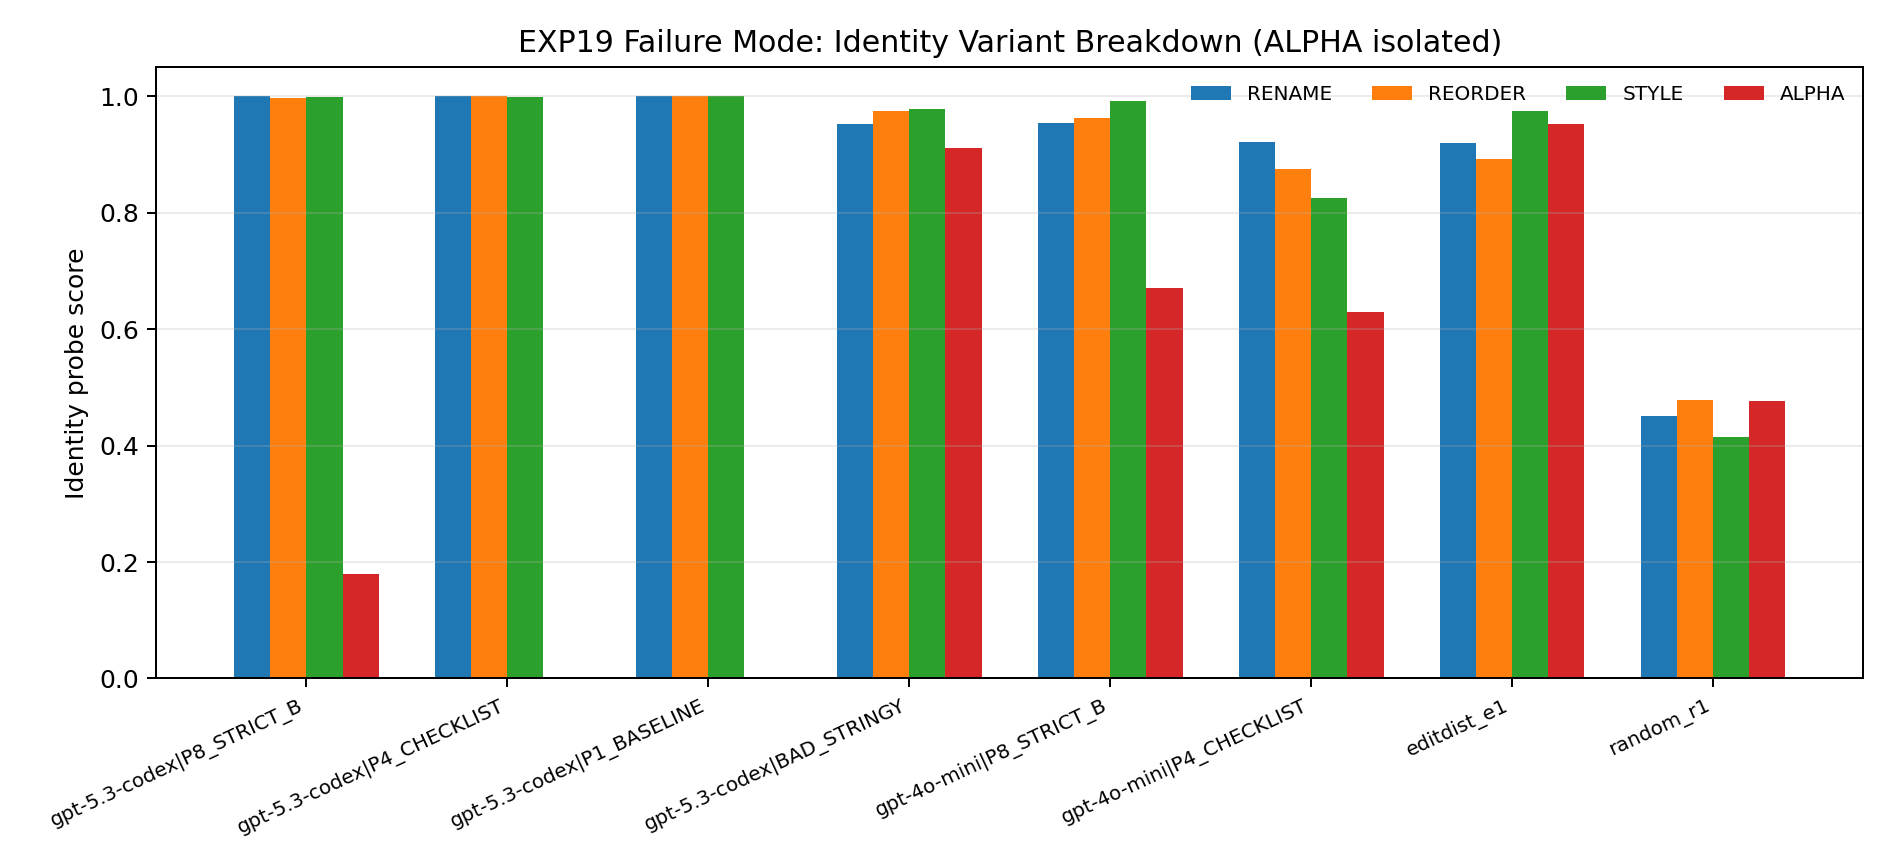
\includegraphics[width=\linewidth]{figures/fig_failure_alpha_variant_breakdown_exp19.png}
    \caption{Failure-mode isolation: identity variant breakdown with ALPHA shown separately.}
    \label{fig:app-exp19-alpha-failure}
  \end{subfigure}
  \caption{\textbf{Low-variance replot package: cleaner main trend + explicit failure separation.}
    The left panel is the ``main story'' plot with lower visual variance; the right panel isolates alpha-renaming sensitivity rather than mixing it into the primary monotonicity figure.}
  \label{fig:app-exp19-main-and-alpha}
\end{figure*}

\begin{figure}[t]
  \centering
  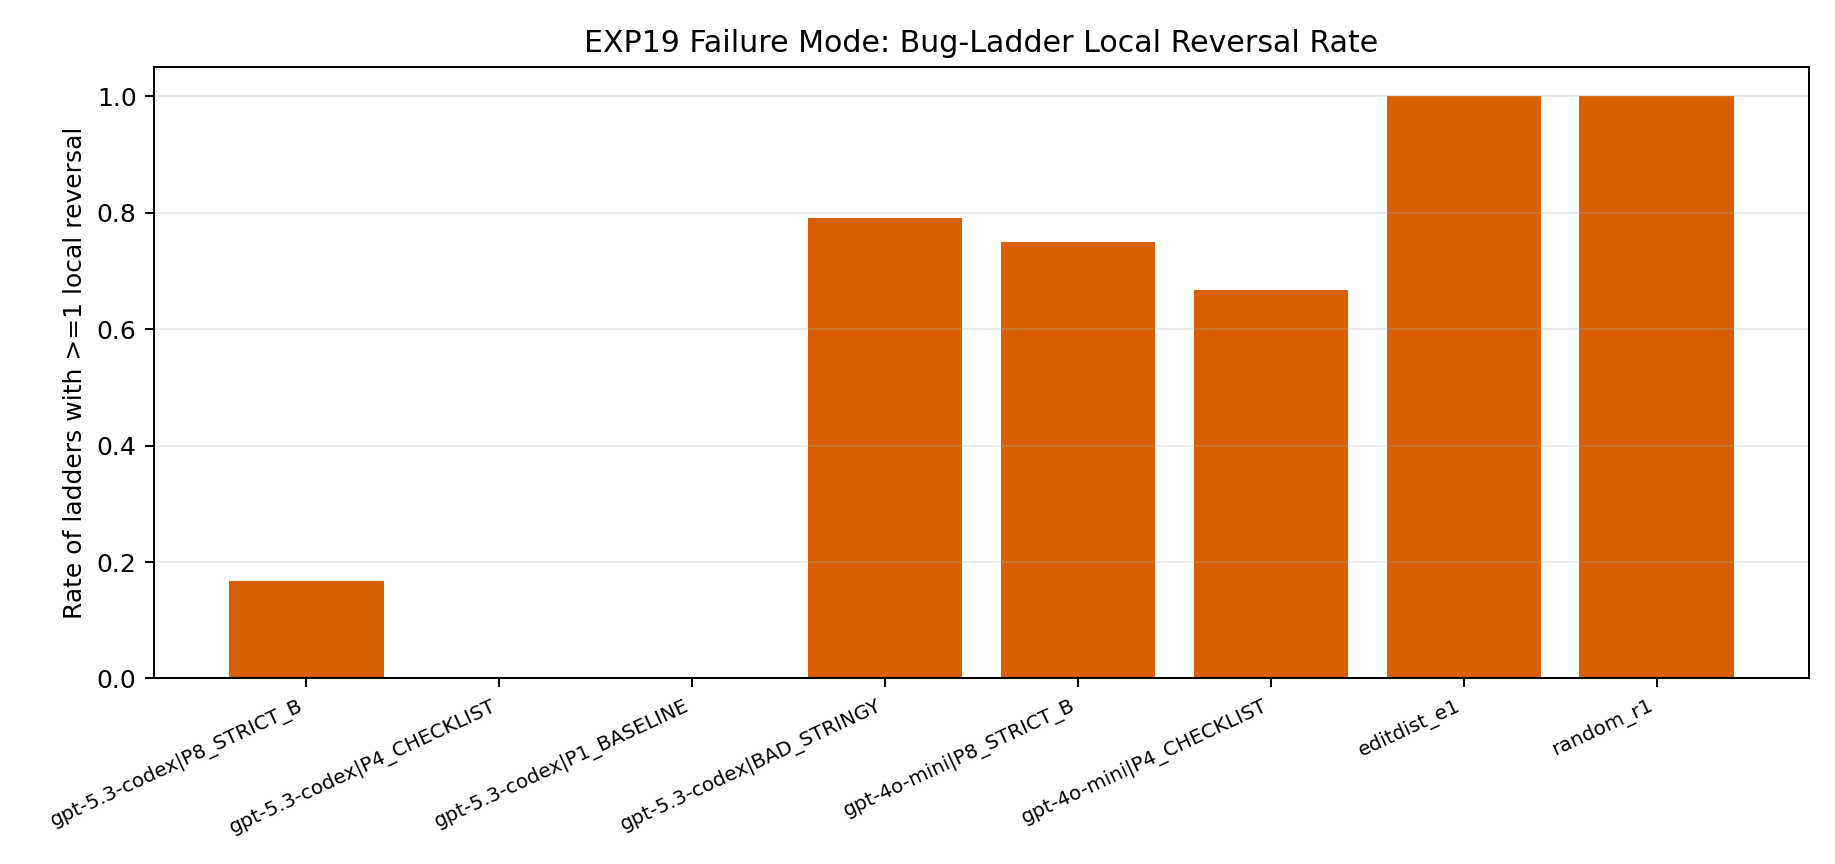
\includegraphics[width=\linewidth]{figures/fig_failure_bug_reversal_rates_exp19.png}
  \caption{\textbf{Failure-mode plot: local bug-ladder reversal rates by judge.}
    This explicitly surfaces where monotonicity fails locally, separating robustness diagnostics from the primary trend plot.}
  \label{fig:app-exp19-reversals}
\end{figure}

%%%%%%%%%%%%%%%%%%%%%%%%%%%%%%%%%%%%%%%%%%%%%%%%%%%%%%%%%%%%
\end{document}
